\documentclass[
  final,
  babelLanguage=hungarian,
  desktopVersion,
  %showtrims,
  %overleaf,
]{anecdote}

\graphicspath{{./assets/photos/300dpi/}}
%\graphicspath{{./assets/photos/92dpi/}}

% Blurb page size: 5 x 8 inch (127 x 203.2 mm)
% Body text: 10.5 / 16 pt

\usepackage{local}

%% Details of the book
%% ===================

\title{Szótlan Vizsgálat}
\subtitle{bevezető a buddhista meditációba és szemléletbe}
\author{Bhikkhu Gambhíró}
\publisher{Kiadó}% TODO
\date{2021-11-07}
\editionInfo{\textit{Első kiadás}, 2022}
\ISBN{000-000-0000-00-0}% TODO update ISBN

% === Metadata ===

\hypersetup{
  pdftitle={\thetitle},
  pdfauthor={\theauthor},
  pdfcopyright={Copyright (C) 2022, \theauthor},
  pdfsubject={},% TODO subject
  pdfkeywords={},% TODO keywords
  pdflicenseurl={https://creativecommons.org/licenses/by-nc-nd/4.0/deed.hu},
  pdfcontacturl={},
  pdflang={hu},
}

%% === Load further packages ===

%% === Hyphenation exceptions and corrections ===

\hyphenation{London Szumédh-áráma}

\begin{document}

\frontmatter

\ifdesktopversion
\desktopCover{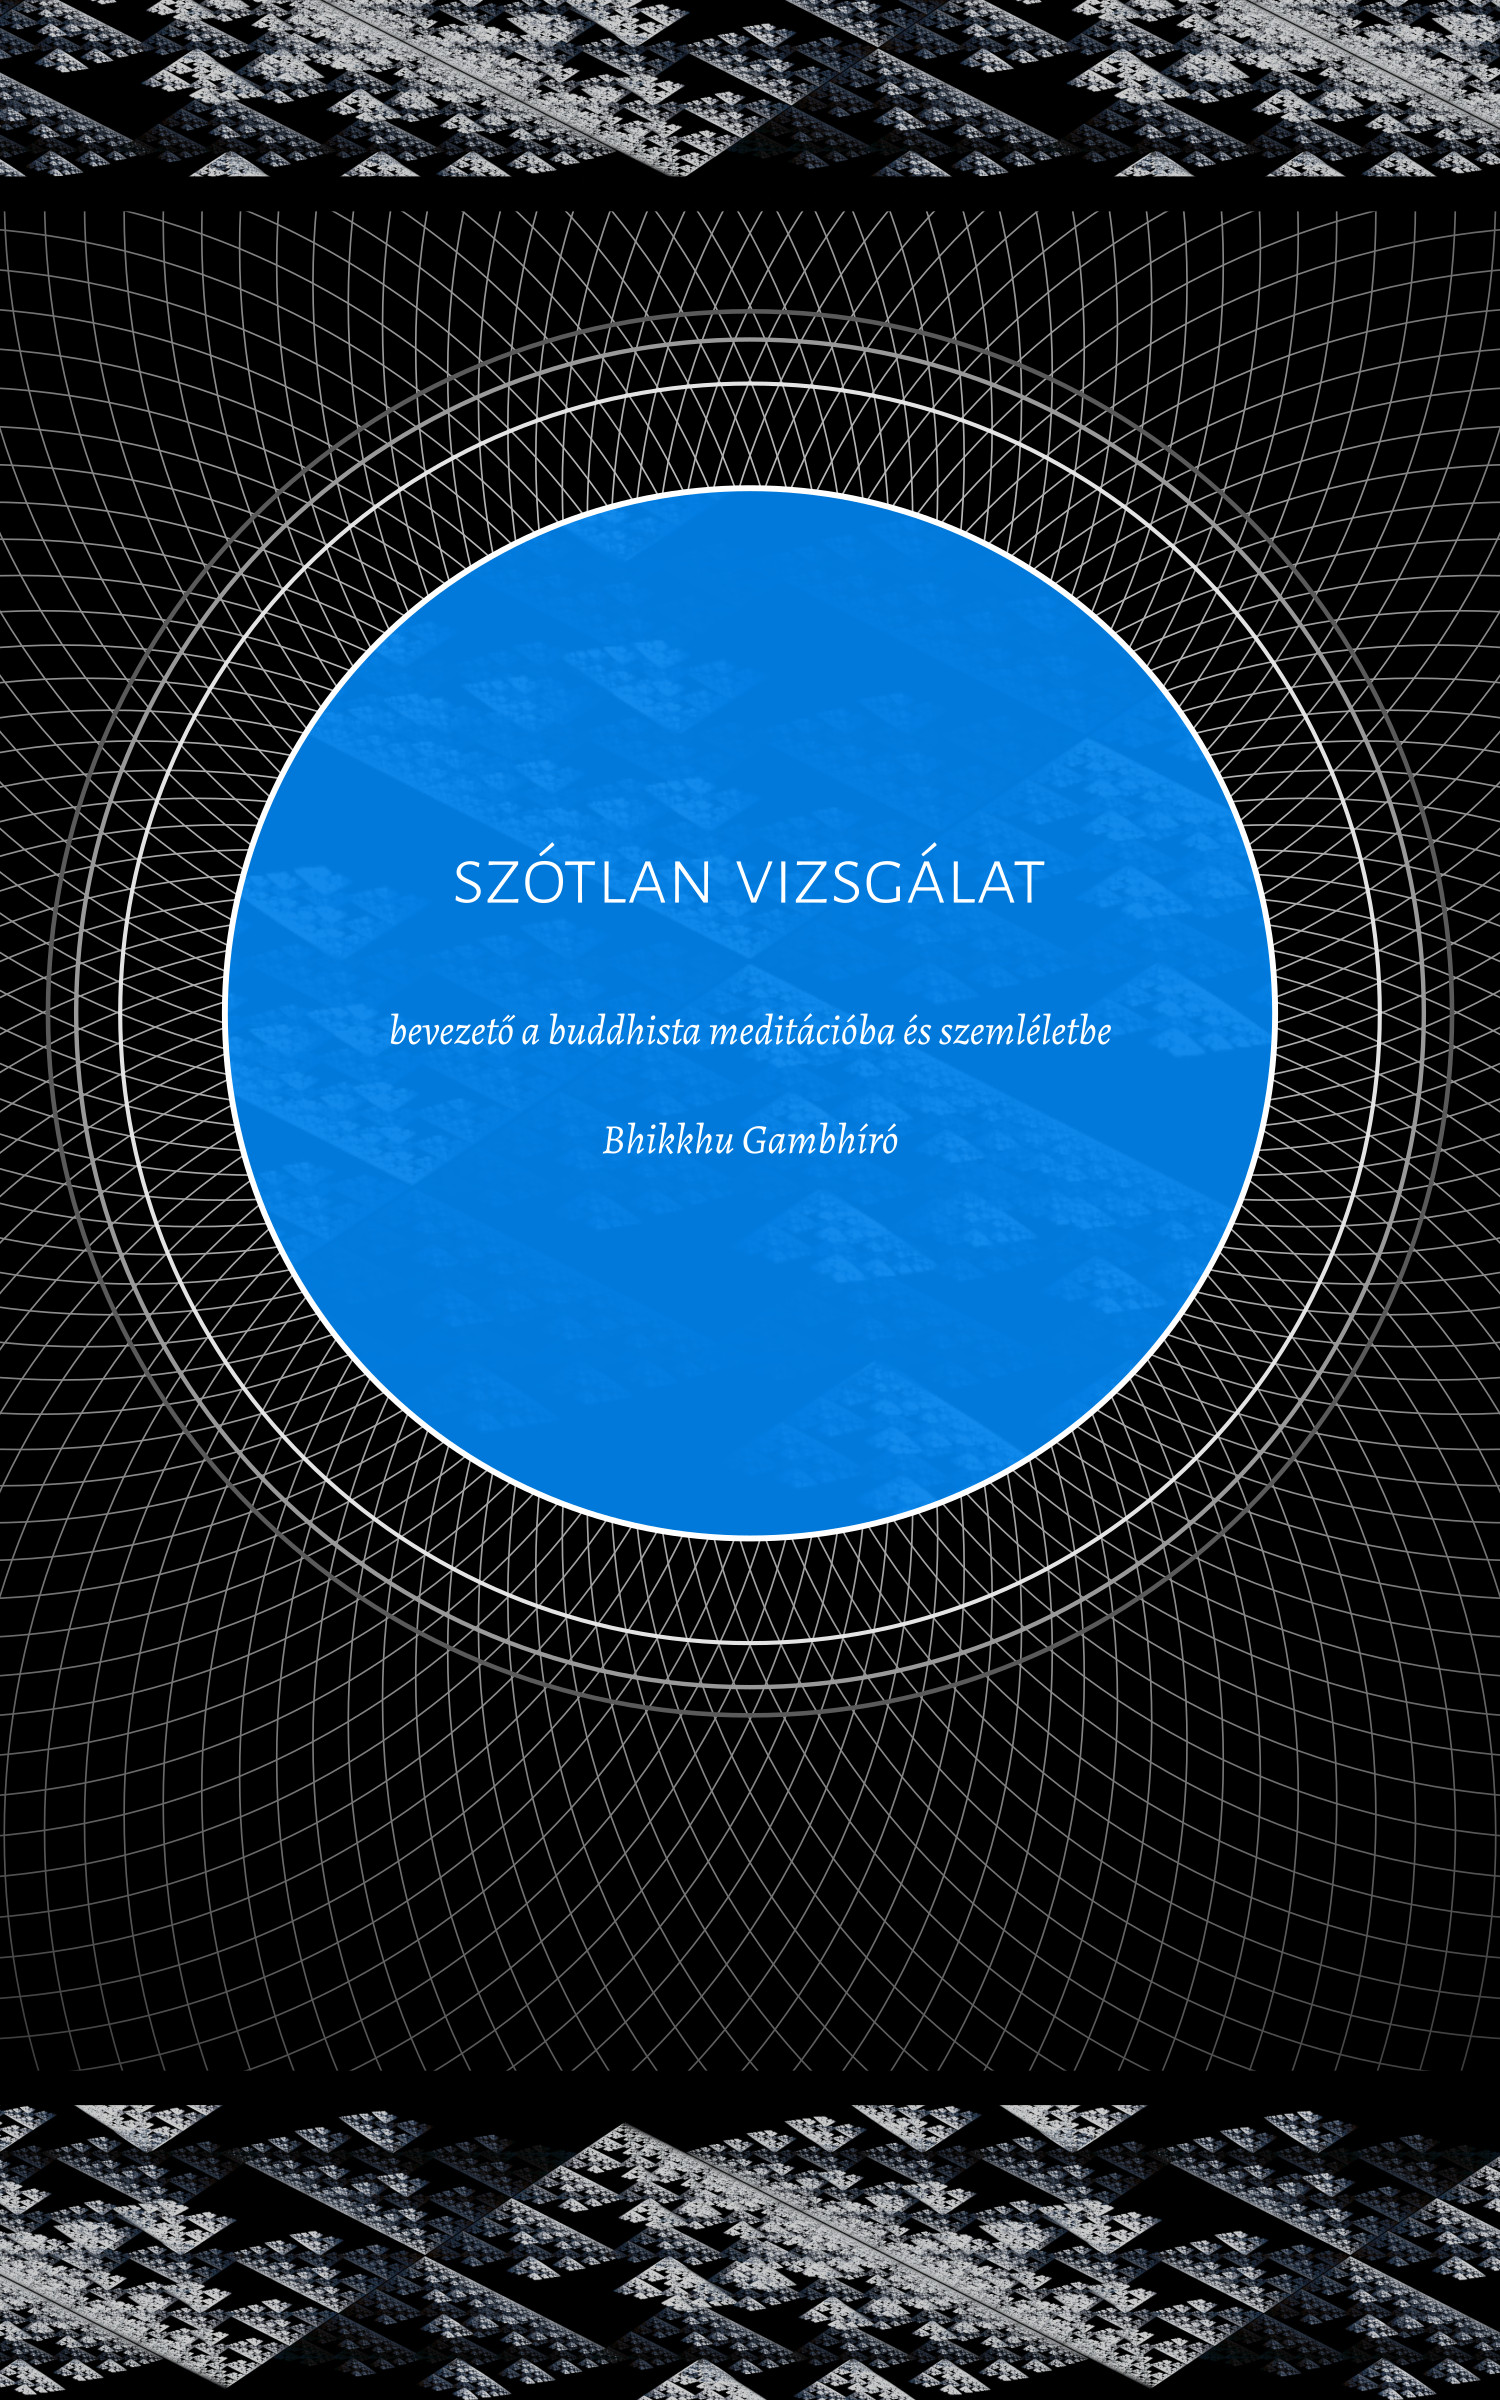
\includegraphics[height=\paperheight]{./desktop-cover-hu.jpg}}
\fi

\cleartorecto
\thispagestyle{empty}
\vspace*{5em}

{\centering

{\Large\alegreyaSansScLightFont\selectfont\MakeLowercase{\textls*{\thetitle}}}\\[5pt]
{\chapterTitleFont\selectfont\itshape \thesubtitle}

\vfill

{\chapterTitleFont \theauthor}

\vspace*{2em}

}



\cleartoverso
\thispagestyle{empty}

{\copyrightsize
\centering
\setlength{\parindent}{0pt}%
\setlength{\parskip}{0.8\baselineskip}%

\thetitle\\
\theauthor

Kiadó: \thePublisher

ISBN \theISBN

Copyright \copyright\ \theauthor\ 2022

Illusztrációk: Madalena Scafuro

\vfill

\hspace*{-5mm}%
\parbox{\linewidth + 10mm}{%
\centering
Ez a Mű a Creative Commons\\
Nevezd meg! - Ne add el! - Ne változtasd! 4.0 Nemzetközi Licenc\\
feltételeinek megfelelően felhasználható.
}

Készült a \LaTeX\ szövegformázó rendszerrel, Crimson Roman és Alegreya Sans betűtípussal szedve.

\theEditionInfo

}



\cleartorecto
\tableofcontents*

\openany
\chapter{Bevezető}

\vspace{-\baselineskip}

Abban az időben, amikor Budapesten tanultam 2005-ben, emlékszem, hogy
kutattam olyan könyvek után, amik segíthetnének használható
perspektívába helyezni zavarodott tapasztalataimat. A magyarázatból és
tanácsból nem volt hiány, de úgy éreztem hiányzott a konkrét irány:
`Érdekes ötletek, de mit \emph{tegyek} és hogyan?' Úgy hiszem, hogy az
útmutatás akkor jó, ha segít abban, hogy többre legyél képes mint
korábban, fényt vet a `mit' és `hogyan'-ra, és talán még a `miért'-re
is.

Az első könyv, ami kapaszkodó pontot nyújtott, Ácsán Szumédhó rövid
könyve volt, \emph{The Four Noble Truths}\footnote{Magyar fordításban:
  \href{https://a-buddha-ujja.hu/books/csittaviveka/hu}{Csittavivéka - A
  csöndes tudat tanítása (a-buddha-ujja.hu)}} (A Négy Nemes Igazság). A
vizsgálódás egy gyakorlati módszerébe nyújtott bevezetőt, a saját
küszködéseinek példáival együtt. Később, amikor Angliában az Amaravati
buddhista kolostorban jártam, a másik könyvét is elolvastam:
\emph{Mindfulness: the Path to the Deathless}\footnote{\href{https://forestsangha.org/teachings/books/mindfulness-the-path-to-the-deathless?language=English}{Mindfulness:
  The Path to the Deathless (forestsangha.org)}} (Éberség: az Út a
Haláltalanhoz), ez is rávilágított sok új dologra.

Azért említem őket itt, mert bizonyos témákat részletesebben tárgyalnak,
és ha ezt a könyvet olvasod, talán ezek is hasznosnak bizonyulnak.

\enlargethispage*{2\baselineskip}

Itt azokat a tanácsokat és tanításokat gyűjtöttem össze, amikről azt
kívánom bárcsak korábban olvastam volna, vagy valaki elmondhatta volna,
az évek során mióta az első könyveket olvastam. A helyes válasz rejtve
marad, amíg meg nem tanuljuk feltenni a helyes kérdést.

Ábrákat és illusztrációkat is mellékeltem, amik a leírások szavai
mellett egy másik csatornán kommunikálnak. Amikor egy ábrát készítek,
olyan kapcsolatokat fedezek fel a kifejezések között, amire korábban nem
gondoltam. Amikor mások ábráit látom, azt mutatják nekem, hogyan
kapcsolódnak a kifejezések egy tágasabb összképet tekintve, és
megkérdezem magamtól, hol található ez a reprezentáció a saját
tapasztalatom térképén.

A meditációs testtartások illusztrációit Madalena Scafuro készítette.

A Tiszt. Thánavaro Bhikkhu figyelmesen ellenőrizte a magyar szöveget.
Hálás vagyok, hogy idejüket és energiájukat ennek a feladatnak
szentelték; ez az útmutató sokat javult munkájuk eredményeképpen. A
könyv bármely része, ami összezavaró és nehezen érthető maradt, a saját
hibámból ered. Ha ezzel találkozol, hagyd magad mögött, és térj vissza a
Buddhához, tanulj a páratlan tanítónktól. Az időtlen igazságot
tanította, a szenvedés teljes megszűnését, mert hitt abban, hogy megvan
a képességünk felismerni azt.

Az évek során sok segítséget és támogatást kaptam első tanítóimtól, akik
a szüleim, illetve szerzetesi tanítóktól és barátoktól. Mi magunk lehet,
hogy alkalmatlannak érezzük magunkat, és nem hisszük, hogy valaha is
boldogok lehetünk, de tanítóink hisznek bennünk és sikert kívánnak
nekünk, hogy túljussunk a zavaron és virágozzon az életünk. Ebben a
szellemben ajánlom fel ezeket a szavakat.

\bigskip

\enlargethispage*{2\baselineskip}

{\raggedleft
Bhikkhu Gambhíró,
2021 November,\\
Sumedháráma Buddhista Kolostor, Portugália
\par}


% Page 1 is the first page of the first chapter.
\mainmatter

\openright

\cleartoverso
\thispagestyle{empty}\mbox{}
\photoFullBleedPlaceholder{%
  TODO: Illustration of sitting posture.%
  \illustration{Ülő Meditáció Tesstartás}%
  \label{illus-sitting-meditation}%
}
\clearpage

\chapter{Légzés}

\keywords{\emph{ānāpānasati} módszer és testtartás röviden}

\noindent A lélegzet érzéseit figyeljük a testben, ez az éber figyelem
az elmét egy stabil tárgy köré gyűjti össze. A test érzései jól
észrevehetőek miközben be- és ki lélegzünk. Ez a módszer
\emph{ānāpānasati} néven ismert, vagyis éberség a lélegzetre.

Miért annyira fárasztó a sok gondolkodás? Az elme egyik gondolattól a
másikig ugrál, de nem tudjuk hova megyünk és így sosem érkezünk meg. A
nyugtalan vágy kimerítő. Az érzéki visszafogottság összegyűjti az
energiát és irányítja azt, nem engedi szétfolyni minden irányba. A
figyelmet egy semleges, egyenletes érzésre irányítjuk, ami lelassítja a
gondolkodó elmét.

Ülhetsz a padlón, a szőnyeget és egy párnát használva, vagy egy széken
is. A padlón ülve, találj olyan helyzetet, ami nem erőlteti túl az
inakat vagy térdeket.

Széken ülve, húzódj előre az ülésen, hogy a hátad ne támaszd a
háttámlának. A támasz befolyásolja a gerinc alakját, és a légzés
ritmusát.

Tartsd a fejet egyensúlyban úgy, hogy a súlya ne húzzon előre. Mivel
gyakran széken ülünk, szokásunk a fejet előre tartani, ami a hátizmokban
hoz létre feszültséget. A fejet egy kicsit hátrahúzva érezzük, hogy
ellazulnak a hátizmok. Jó, ha az áll kissé behúzódik, de nem kell
erőltetni.

Ülj egyenesen, kiegyensúlyozott testtartásban, a vállakat ellazítva. Jó
tartással a légzés könnyű és egyenletes.

\clearpage
\null\thispagestyle{empty}%
\photoFullBleed{sitting.jpg}%
\illustration{Ülő Meditáció Tesstartás}%
\label{illus-sitting-meditation}%
\clearpage

A test csontjai úgy ülnek egymáson mint egy kövekből rakott torony. A
csípő-csont a párnán nyugszik, a gerinc a csípőn, a gerinc-korongok
egymásra rakva, a tetején a koponya, az egész torony középvonala
óvatosan egyensúlyban tartva.

Ha óvatosan ki van egyensúlyozva, és a súlypont középen van, nem
szükséges az izmok erejével húzni-vonni a testet, hogy megtartsuk. A
gravitáció elég ahhoz, egyenesben tartsa.

Belégzéskor, a hideg levegőt először az orrhegynél érezzük. Hagyd, hogy
a hasizmok irányítsák a levegővételt, ahelyett, hogy a mellkast tágítva
növelnéd a térfogatot. A levegő áthalad a tüdőn, és a has kitágul; ez a
légzési módszer csökkenti a szívritmust és feszültséget. Ellazítjuk az
izmokat, és a levegő az orron át távozik. Nem kell ezt precízen
irányítanunk, elegendő finoman utalni erre a ritmusra. A test magától is
tudja hogyan kell lélegezni, visszalépünk és figyelünk, mintha
hullámokat néznénk ahogy besodródnak a partra, majd visszahúzódnak.

Nem kell megmondanunk magunknak mit gondoljunk és mit érezzünk. Ha
tiszta gondolatokat akarunk, legjobb először csendben lenni és figyelni.
Csendben ülünk és pihenünk egy kis ideig. Mikor elhallgatunk, vagy
tiszta gondolatok jönnek maguktól, vagy az elme elégedett lesz a
csenddel együtt maradni.

Visszafogottság és irányított figyelem szükséges a tiszta, tudatos
gondolathoz -- és ez békés örömet hoz magával. Az elme elégedett és
boldog, nem érzi szükségét a sok belső párbeszédnek. Leülni és
lélegezni, a csendet hallgatni magában is egy hibátlan öröm.

Megalapozzuk a tiszta szándékot, hogy a meditáció tárgyával maradunk és
más ügyeket későbbre hagyunk. Segít a nyitott hozzáállás, erővel
kényszeríteni magunkat nem elég érzékeny, hogy lássuk mi történik.
Akaraterővel irányítva a meditáció merevvé válik, és az elme
akadályozott lesz. Mintha gyorsan akarnánk menetelni merev lábakkal, és
felbukunk a kavicsokban.

A tiszta elme és jó elhatározás érzése nyugodt és hűvös, nyitott a
változásra. Az erőltetett küszködés érzése elfoglalt és forró, szűk a
látótere.

\keywords{hozzáállás a módszerhez, az elme nem egy kávégép}

Tanulunk új tényeket az elméről azzal, hogy a légzést figyeljük?
Emlékszem, amikor nekiültem és azzal küszködtem, hogyan kellene
\emph{helyesen} meditálnom. Folyton ezen gondolkodtam és a légzésemen
változtatgattam hogy javítsak a meditációmon, arra számítva, hogy egy
nap majd valahogy megnyomom a helyes gombokat, és a helyes módon
lélegezve elkezdek új információkat, új tényeket megismerni az elméről.
Elég fájdalmas folyamat volt, és teljesen eredménytelen.

A tudást keresve analizálunk, és közben lemaradunk arról, ami történik.
Gondolj egy beszélgetésre, mikor a másik folyton azt kérdezi,
``Miért?'', minden mondatod után -- a beszélgetés sehova nem jut
hallgató figyelem nélkül. Ezt tesszük magunkkal miközben túlagyaljuk a
meditációt; nem is csoda, hogy fel akarunk ugrani az ülőpárnáról és
megmondani a kommentáló elménknek, hogy hagyja abba és figyeljen
csendben.

A tanítóink utasításai a figyelmünk olyan irányítására vezetnek rá,
amivel a magunk számára felfedezhetjük a megértést.

Tanulunk az olvasott vagy hallott utasításokból, de amikor
\emph{pontosan, precízen, helyesen} próbáljuk követni ezeket, olyan,
mintha a kézikönyvet olvasnánk egy kávégép működtetéséhez: `Ha megnyomom
ezt a gombot, mindig ilyen kávét kellene készítsen'.

Ezt a hozzáállást az motiválja, hogy irányítani és manipulálni akarjuk
az élményeinket, de frusztrációt tapasztalunk, mert természetük szerint
nincsenek az irányításunk alatt. Már előre eldöntöttük mi lesz. Azt
akarjuk látni, amit \emph{gondolunk}, hogy történnie kellene, és nem
látjuk ami \emph{valóban} történik, ezért azt gondoljuk a gép nem
működik, vagy mi használjuk rosszul.

Emlékeztethetjük magunkat, hogy lehetséges, hogy nem tudunk mindent. Nem
tudjuk mi fog történni. Lazíts a tartáson, gyakorold a hozzáállást ami
megáll és figyel.

\keywords{BUD-DHÓ mantra, erőfeszítés és frusztráció}

Kezdhetjük a BUD-DHÓ mantra gyakorlásával, magunkban ismételve a be- és
kilégzéskor. `Buddhó' azt jelenti, `aki éber, aki megismer'. Segít
megállni és figyelni.

Ez felébreszti az elmét, hogy ismerje önmagát ahogy épp most van. Az
ébredés mindig helyes -- nem tudod elrontani. Az elme felismeri a saját
változó természetét, a gondolatok szavai szükségtelenné válnak, és a
figyelem megtalálja a szótlan kérdést ami a jelennel együtt marad.

Az erőfeszítés szükséges, és az elme akadályai miatt nehéz feladatot tud
jelenteni, hogy ne adjuk fel a gyakorlást. Újra és újra, visszatérünk az
elméhez ami éber a jelen tapasztalatra és ez irányítja az erőfeszítést,
az akaratos törtetés helyett egy cél felé.

A frusztráció és csalódás hasznos jelzések arra, hogy figyeljünk -- a
legjobb, amikor olyan dolgot kell megtanulnunk, amire nem számítottunk,
hogy erre jobban kell figyelnünk.

Nem szükséges sokat olvasnunk, vagy sok mindenre emlékeznünk. Kevés
információra van szükségünk, de kifejleszteni a jártasságot ezekben sok
gyakorlást igényel. Gyakori hibánk, hogy nem állunk meg, hogy velük
maradjunk, és kicsomagoljuk a jelentésüket arra, hogy felismerjük a
pillanatnyi helyzetünket, \emph{mit tegyünk} és \emph{milyen módon
tegyük azt}.

Egy sor tény, ha nem építjük be őket, nem érnek le elég mélyre, hogy a
szív és elme tapasztalatainak gyökereit kezeljék, és nincsenek ránk
hatással. A lélegzet figyelése megállít minket, és megnyílik a
figyelmünk, ami képes ezt elérni. Az észrevételek és megismerés
fokozatos lehet, mint amikor közel kell hajolnunk valamihez, hogy
lássunk egy lényeges részletet, de minden lépés, amivel összekötjük a
saját tapasztaltunkat a tanítás szavaival, érdekes és tovább vezet.

A Buddhának egy egyszerű üzenete van számunkra: ébredj fel, ne
ragaszkodj, nem kell szenvedned. Ezt csomagoljuk ki, egyre szélesebbre
tárva.

\section{Vezetett meditáció}

\keywords{\emph{ānāpānasati} módszer, ülő meditáció, ülő tesstartás}

\enlargethispage*{\baselineskip}

Igazítsd ahogy ülsz, és találj egy kiegyensúlyozott testtartást: a
tartásod egyenes legyen, stabil de nem feszes helyzetben, a fej legyen
egyensúlyban és ne dőljön előre. A tartásod engedje a nyitott, könnyű
légzést.

Határozd el, hogy erre az időre félreteszed a mindennapi
tevékenységeket. Válaszolhatsz a megszakító gondolatokra, `Ez nem a
megfelelő idő, később vissza fogok erre térni amikor az idő alkalmas
rá.' Hosszabb, mint az, hogy `Csend legyen!', de barátságosabb magunkkal
szemben. Ez megalapoz egy tiszta szándékot az elmében, mint elpakolni az
asztalról mielőtt dolgozni kezdünk.

Vegyél egy mély lélegzetet, és figyeld, hogy érzel-e feszültséget,
valamit ami akadályozza vagy korlátozza a légzést. Ha úgy érzed, a
légzés könnyű és nyitott, a testtartásod megfelelő. Nem kell különleges
módon ülnöd.

Figyelj a légzés testi érzéseire. Engedd, hogy a test szabályozza a
légzést, mi csak figyeljük és hagyjuk ellazulni, arra figyelve ami éppen
történik.

A jó testtartás és a nyugodt, könnyű légzés egy csendes és örömteli
érzés, mint leülni a parkban egy padra egy séta után. Semmi különös
dolgunk nincs, és ez az egyszerű, csendes ülés magában is öröm.

A légzést nem irányítjuk olyan precízen, mint egy pránajáma vagy jóga
gyakorlat közben, viszont érdemes figyelni milyen testi ritmus irányítja
a légzésünket.

Ha a légzést a mellkas tágulása és összehúzódása irányítja, mintha nagy
erőfeszítésre készülnénk, ez mozgásra ösztönöz és aktívabban gondolkodó
elmét produkál. Megnyugtató hatással van, ha inkább a has feletti
rekeszizom irányítja a légzést. Ha egyszer megvan a ritmusa, hagyd a
testet, hogy magától folytassa.

\enlargethispage*{\baselineskip}

Belégzéskor, a levegőt először az orrhegynél érezzük. A hideg levegő
lefelé áramlik a légcsövön. A has kifelé mozdul, engedve a rekeszizom
tágulásának. A mellkas emelkedik, miközben a tüdőt kitölti a levegő, de
nem kell nagyra tágítani a mellkast. Nyugodtan ülünk, érezhetjük a
szívverés halk ritmusát.

\clearpage
\null\thispagestyle{empty}%
\photoFullBleed{breathing.jpg}%
\illustration{Légzés Technika}%
\label{illus-breathing}%
\clearpage

Kilégzéskor az izmok ellazulnak, a meleg levegő felfelé áramlik a
légcsövön, és az orron át távozik.

Nem szükséges ezeket a lépéseket gondolatban kifejezni, lazíts és
figyeld, ahogy az érzések megjelennek a testben. Eltart pár percig, amíg
a test megállapodik. A szívverés lecsillapodik, és a légzés egyenletes
és könnyű lesz.

Hagyd, hogy a test maga szabályozza a légzést. Amikor egy véleménnyel
állunk hozzá, hogy a légzésünk rövid legyen, vagy hosszú, az merevvé és
erőltetetté válik. Fel akarjuk fedezni a tapasztalatainkat, nem
megszabni, mik legyenek azok.

A test jobban tudja hogyan kell lélegezni, mint mi. Egyenletesen fog
lélegezni, ha hagyjuk. Lépj egyet vissza és fordítsd meg a figyelmet,
hallgatózz ahelyett, hogy utasítasz. Belégzés, kilégzés, mit érzel a
testben?

Nincs semmilyen meghatározott érzés, amit tapasztalnod kell. A szándék
az, hogy adj időt, és engedj teret annak, hogy a tapasztalataiddal
maradj.

Egyensúlyban önmaga középpontjában, ismerni a jelen pillanat
egyszerűségét. Ha úgy érzed, hogy valamit teljesítened vagy javítanod
kell, ez mindig egy hozzáadott dolog, valami amit mi hozunk létre. Mi
hozzuk létre az elvárást, hogy változtatnunk kell, ki kell valamit
javítanunk, irányítanunk kell. Ez mindig az időhöz kötött, valamit
elvárunk, hogy történni fog.

\enlargethispage*{2\baselineskip}

A jelen pillanatban minden mozgásban, változásban van. Az azonnal, a
jelenben megtapasztalható élményben nincsenek célok. Nincsenek a jövőben
megjelenő eredmények, csak \emph{ez, itt} van. Azok az elvárások, amiket
magunk számára produkálunk, szétfoszlanak, amikor visszafordítjuk a
figyelmet, és a jelent figyeljük.

Visszatérünk a figyelemhez, ami az itt és most tapasztalathoz kötődik.
Az érzékeken keresztül felismeri a világot. Ebben a figyelemben a
kétségek, kérdések, emlékek, nem súlyosak. Nincs olyan súlyuk, nincs
olyan sürgető jelentőségük, ami minket kimozdítana az egyensúlyból. Ez
az éber figyelem egy biztonságos hellyé válik, ahol maradni tudunk.

Lehet, hogy sok kusza gondolat jár az elmében. Határozd el mit fogsz
gondolni, ahelyett, hogy hagynád az elmét körbe-körbe járni. Például
használd a BUD-DHÓ mantrát. A belégzéskor, gondold BUD-, kilégzéskor,
-DHÓ. Ha a gondolkodás nem csillapodik le magától, ez oldalkorlátot és
fekvő-rendőrt rak le, hogy az úton maradjunk és lassítsunk.

\keywords{aktív és nyugodt elme, kavargó érzelmek, a jelen egyszerűsége}

Belélegzünk, maradunk a jelen egyszerű tapasztalatával: ennyi elég.

Kényszereket érzünk, vágyakat és aggodalmakat, úgy érezzük, `erre
szükségem van', `én ilyen vagyok', `olyannak kellene lennem'. Ezeket
éberen szemlélni tudjuk, nem kell belekeverednünk a történetbe. A
légzéssel maradunk, és figyelmünket a tapasztalat felé fordítjuk, ami
éppen történik.

A testi éberség egy szilárd alap, megnyugtató és átrendezi mi az
értékes. Ha a tapasztalatod békés, boldog és elégedett, maradj vele.
Nincs abban semmi rossz. Ez egy olyan boldogság, ami nem kötődik a
ragaszkodáshoz, nem függ attól, hogy megszerezzünk vagy elérjünk
valamit. Ez a boldogság az érzékek elvonultságából ered, visszatérve az
egyszerűséghez, megismeri és együtt marad a jelennel. Az elme éber,
nyugodt és elégedett.

A meditáció a kavargó érzelmeket is a felszínre hozza, és ez jól van
így. Azt látjuk, amit eddig nem engedtünk magunknak, hogy lássunk. Nincs
szükség arra, hogy válaszokat és megoldásokat keressünk meditáció
közben. Az érzelmeket nem a személyes történetünk szintjén vizsgáljuk,
hanem alapvetőbb szinten, mint az elme és szív állapotait.

Magunkat látjuk bennük, sajátunknak tekintjük ezeket, és ebből hozunk
létre egy személyt, akinek a történetét irányítani akarjuk. A jelen
tapasztalatban viszont sem az érzés, sem az elmeállapot nem jelenti be
magáról, hogy kinek a nevéhez tartozik. A szenvedés és nehézség ebből a
ragaszkodásból és zavaros nézetből ered. Nyitni kell az elmét a
változásra, és elengedni a ragaszkodást.

\keywords{jótékony gondolatok, túl komoly hozzáállás}

Az erény, a nagylelkűség ellazítja az elmét, a moralitás pedig stabil
alapot ad. Gondolhatunk jó tettekre, amit adtunk és kaptunk,
emlékezhetünk azokra, akikre jó példaként tisztelettel nézünk fel.

Ha azt veszed észre, hogy feszült vagy, szigorú és cinikus a hangulatod,
igazíts a testtartáson, hogy kicsit lazább legyen.

Olyan komolyak tudunk lenni abban, hogy egy párnán ülünk, kész vicc ránk
nézni. Csendben dörzsöld meg a füleid, vagy masszírozd meg az arc
izmokat az ujjaiddal, ez serkenti a vérkeringést. Emlékezz a
nagylelkűségre. A kolostorban gyakran a világi barátaink azok, akik
eljönnek főzni és felajánlani a napi ebédet a közösség számára. Nagy a
sürgés-forgás amíg a konyhában vannak, és amikor végeztek,
megkönnyebbültek, lazítanak és mosolyognak.

\enlargethispage*{\baselineskip}

Felidézni jó tetteinket, egyszerű kis dolgok esetében is, ellazítja az
eredményekre szomjas elmét. Képzeld el mi történne, ha valaki
százszorosan megadná neked az eredményt amit akarsz, mintha megnyernél
egy megvilágosodási lottót. Akkor hogy meditálnál? Valószínűleg közel
úgy mint most, csak lazábban.

A nagylelkűség enged felismerni, hogy van elég terünk, nem kell
erőlködnünk, hogy mások elé jussunk. Van jóság a világban és
felhagyhatunk a nagy sietséggel. Örömteli érzés felidézni a családunk,
rokonaink és barátaink nagylelkűségét is, de még amikor egy ismeretlen
embert látunk segíteni egy másik ismeretlennek, az is előcsal egy
mosolyt.

\keywords{kétség a meditációban, érzékek befelé fordulnak}

`Hogy tudom megcsinálni?' Közelítsd meg másként, és inkább azt kérdezd,
`Tudok rá figyelni?'

A légzés érzete megállít. Visszakerülünk az elejére, ahol nem tudjuk mi
lesz. Egy üres és tágas helyre kerülünk így, ahol magunk vagyunk és van
időnk ott megállni.

A légzésre figyelve az érzékek befelé fordulnak. A szem látja a
színeket, de a látás befelé irányul, nem akar kívül színeket és formákat
keresni. A fül hallja a hangokat, de a hallás befelé fordul és nem
keres. A test érzi a hideget, meleget, a ruhák felületét és a csontok
merev súlyát. A légzés közben figyeljük ezt és hagyjuk a testet
lenyugodni, hagyjuk az elmét befelé fordulva elcsendesedni.

\enlargethispage*{2\baselineskip}

\keywords{hűvös víz szétárad a tóban, a tapasztalat tartalmazza a világot}

Az érzéki visszafogottság összegyűjti az energiánkat és nem engedi
szétfolyni minden irányba. Mint egy tó, aminek nincsenek ki- és bevezető
folyásai, határait körben a völgy szabja meg. Csupán egyetlen, a földből
feltörő forrásból kap hűvös, friss vizet. Amikor eső esik, némi víz kis
erekben a tóba fog folyni, de mivel nincs kifolyása, mind a tóban fog
megállni és a völgy határt szab neki. A tó vize nyugodt marad, és a
forrás hűvös vize az egész tóban szét fog áradni, áthatja annak minden
részét.\footnote{\href{https://a-buddha-ujja.hu/dn-2/hu/csimma-vilmos}{DN
  2}, A szerzetesi élet gyümölcsei}

Az érzés és tudat a testtől függ, nem tudunk hozzátenni vagy elvenni
belőle. A tapasztalat minden légzésben teljes, a testtel kezdődik és
azzal lesz vége. Ez a világ, ami érzésekből áll, ebben teljes -- minden
ami vagyunk, vagy amivé valaha válhatunk, ezen belül van.

\keywords{a tudatosság megállítja a kényszert}

Amikor szenvedünk, tudjuk, hogy van itt valami, amit nem értünk. Nem
értjük, hogy egy dolog hogyan jött létre a másikból, hogy egy dolog az
irányításunk alatt van, a másik pedig nincs.

Amikor nem látjuk, ugyanazt a mintát ismételjük, mint egy programot, és
ugyanazt a szenvedést újra és újra létrehozzuk. Panaszkodunk, hogy
`Miért van ez mindig így?' Ugyanazt a dolgot tesszük újra és újra, és
nem vesszük észre.

Közelebbről megvizsgálva felismerjük, hogy az egyik dolog a másiktól
függ. Akkor látjuk a lehetőséget, hogy szabadon abbahagyhatjuk. Így
visszatérünk a csendes elégedettséghez.

\keywords{nyugtalanság, önkritizálás, jó szándékkal kezdeni, rugalmas hozzáállás}

Amikor már egy ideje meditálva ülünk, gyakran elkezdjük bonyolítani a
dolgot. Honnan jön ez a nyugtalanság, hogy nem tudunk egy egyszerű
dologgal együtt maradni? Figyeld meg, ahogy az egyszerűbe vetett hit
megváltozik. Elkezdünk valamilyen szempontról vagy kérdésről
gondolkodni, és a kétség és önkritizálás megállít mindent.

\enlargethispage*{\baselineskip}

Nem komikus ez? Olyan elkötelezetten tudjuk kritizálni magunkat, mintha
egy túlemelkedett élmény lenne az, hogy fájdalmat okozunk magunknak. De
úgy érezzük, erőlködnünk kell \emph{valamin}, meg kell törjük az egónkat
és el kell engedjünk mindent! Talán csak ezt az egy módszert ismerjük,
nem is tudjuk milyen lehet nem ilyennek lenni.

Az elején megvan az önmagunkkal szembeni jó szándékunk és rugalmas
hozzáállásunk, de a végén csak keménység és bírálat marad. A fiatal fa
friss és rugalmas, könnyen hajlik ahogy nő, de az öreg fa kemény és
száraz amikor elpusztul.

Térj vissza az elejére, ahol megvan a kezdővel szembeni türelmed és
kedvességed. Az elején még nem vártad el magadtól, hogy tudnod kell, és
a hallgató figyelemre hagytad, hogy lásd, mi történik. Nem tudjuk, mi
van itt, amíg meg nem nézzük, hogy lássunk. Ez a látás és figyelem a
friss megismerés. Engedd magadnak, hogy mindig az elején legyél.

\clearpage
\figurepagelayout

\begin{figure}[h]
\caption{Éberség a Légzésre (\emph{Ānāpānasati})}\label{fig-mindfulness-of-breathing}
\bigskip
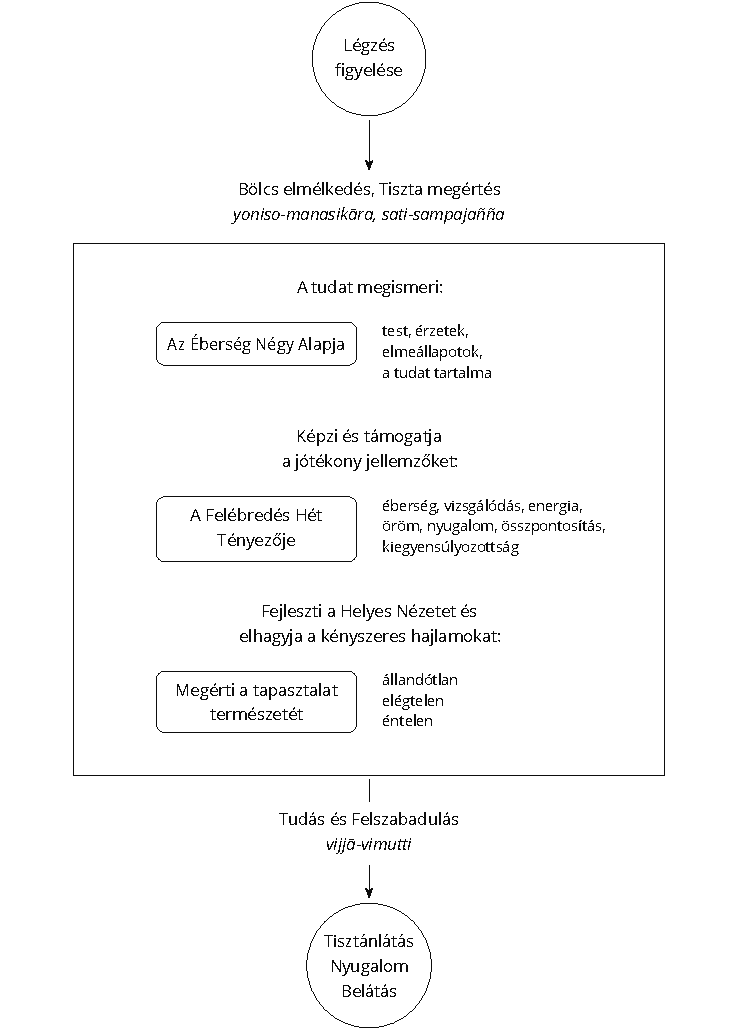
\includegraphics[width=\linewidth]{./manuscript/tex/diagrams/mindfulness-of-breathing-hu.pdf}
\end{figure}

\clearpage
\normalpagelayout

\section{A Lélegzés Tudatosságáról (részlet)}

{\centering
\emph{\href{https://a-buddha-ujja.hu/mn-118/hu/farkas-pal}{MN 118}, Ānāpānasati Sutta}
\par}

{
\setlength{\parindent}{0pt}\setlength{\parskip}{5pt}
\fontsize{9.5}{14}\selectfont

Szerzetesek, a légzés tudatossága, fejlesztve és újra meg újra gyakorolva nagy
eredményt, nagy hasznot hoz, szerzetesek, a légzés tudatossága, fejlesztve és
újra meg újra gyakorolva kiteljesíti a tudatosság négy megalapozását, a
tudatosság négy megalapozása, fejlesztve és újra meg újra gyakorolva kiteljesíti
a megvilágosodás hét tényezőjét, a megvilágosodás hét tényezője, fejlesztve és
újra meg újra gyakorolva kiteljesíti a tisztánlátásból fakadó megszabadulást.

És fejlesztve, szerzetesek, újra meg újra gyakorolva, hogyan hoz a légzés
tudatossága nagy eredményt, nagy hasznot?

E tanítás szerint a szerzetes kimegy az erdőbe, vagy egy fa tövébe, vagy egy
néptelen helyre, keresztbetett lábakkal leül, kiegyenesíti a testét, felkeltvén
tudatosságát (maga előtt).

Tudatosan lélegzik be, tudatosan lélegzik ki.

\textbf{A Test}

Hosszan be- és kilélegezvén tudja,\\ `Hosszan lélegzem be \& ki'.

Röviden be- és kilélegezvén tudja,\\ `Röviden lélegzem be \& ki'.

Így gyakorol:\\ `A teljes testet tapasztalva lélegzem be \& ki'.

Így gyakorol:\\ `A testi képző erőket elnyugtatva, lélegzem be \& ki'.

\clearpage

\textbf{Az Érzések}

Így gyakorol:

`Örömöt tapasztalva lélegzem be \& ki'.

`Boldogságot tapasztalva lélegzem be \& ki'.

`A tudati képző erőket tapasztalva lélegzem be \& ki'.

`A tudati képző erőket elnyugtatva lélegzem be \& ki'.

\textbf{A Tudat}

Így gyakorol:

`A tudatot tapasztalva lélegzem be \& ki'.

`A tudatot felvidítva lélegzem be \& ki'.

`A tudatot összpontosítva lélegzem be \& ki'.

`A tudatot megszabadítva lélegzem be \& ki'.

\textbf{A Tudat Tartalma}

Így gyakorol:

`A mulandóság fölött szemlélődve lélegzem be \& ki'.

`Az elenyészés fölött szemlélődve lélegzem be \& ki'.

`A megszűnés fölött szemlélődve lélegzem be \& ki'.

`Az eloldódás fölött szemlélődve lélegzem be \& ki'.

\bigskip

Ily módon hoz a légzés tudatossága, fejlesztve és újra meg újra gyakorolva, nagy eredményt, nagy hasznot.

}

\chapter{Megértés}

\keywords{tények és tapasztalat, kétség, tények halmozása}

\noindent Részekre osztjuk az ismeretet és fokozatos lépésekben
beszélünk a gyakorlásról, de a megértés egyszerre történik. Az
észrevétel azonnal történik -- az `Aha!' pillanat, amikor eloszlik a
köd. Kezdetben szükséges némi információ, de emlékszünk arra, hogy a
tanítás igazságát mindenki a saját tapasztalatán keresztül éli meg. A
meditáció gyakorlásában azok a tények hasznosak számunkra, amik
\emph{itt-és-most} tények, amit a jelen pillanatban megismerünk.

Ha csupán külső információra támaszkodunk, vagy folyton egy újabb
élményre várunk, sosem érkezünk meg oda, ahol megállhatunk. Ez a
függőség kimerítő. Egyre több kétséget és mentális nyugtalanságot hoz
létre. Hiába halmozunk fel egyre több tényt, egyre keserűbben érezzük
magunkat, és erősödik a belső hiányérzet. Nem több információra van
szükségünk, hanem ennek a szükségnek az elengedésére. Akkor tudunk
nyugodtan megállni.

\keywords{érzéki tapasztalat, azonosulás}

Az emlékek, érzékelés és elvárások egy tapintható erővel húznak-tolnak
minket. Míg az élmények maguk eltűnnek, a kényszer sosem pihen: máris a
következőt akarjuk. Hogyan lehetnek ezek a jelenségek olyan meggyőzőek,
hogy folyton húznak minket előre? Az táplálja a folyamatot, hogy
\emph{magunkat látjuk bennük.} Úgy látjuk, hogy ezek vagyunk, ezek
voltunk, ezek leszünk, és mivel szüntelenül változnak és felbomlanak,
egyre tovább folytatjuk, várjuk a következőt.

\clearpage
\figurepagelayout

\begin{figure}[h]
\vspace*{-15pt}
\caption{Érzet és Azonosulás}\label{fig-feeling-identification}
\bigskip
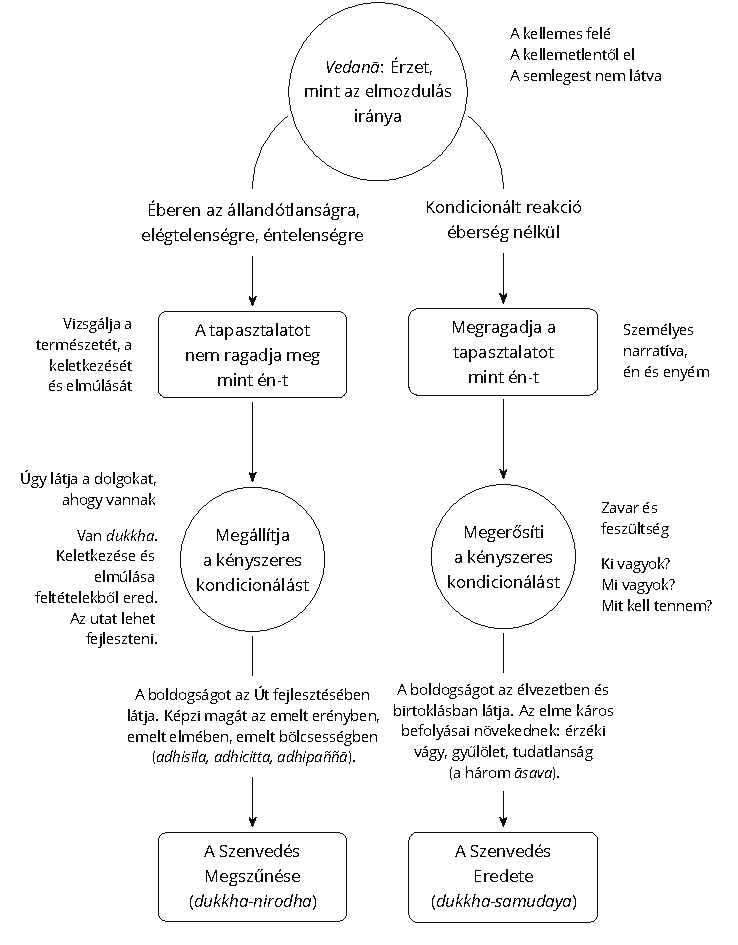
\includegraphics[width=\linewidth]{./manuscript/tex/diagrams/feeling-identification-hu.pdf}
\vspace*{\baselineskip}
\end{figure}

\clearpage
\normalpagelayout

Mi lenne, ha egy nap úgy ébrednénk fel, hogy semmire sem emlékszünk a
múltból? A tapasztalatunkat ilyen állapotban is megragadnánk, mint
\emph{én és enyém}. Annyira kiborító lehetne, hogy félelemtől bénulva
feküdnénk amíg meg nem tudunk ragadni valamilyen történetet, ami
megmagyarázza hol és kik vagyunk. Nem is kell elveszíteni a memóriánkat,
hogy ezt megfigyeljük: utazás közben lekésni egy fontos csatlakozást is
elég ijesztő lehet, hogy így érezzük magunkat, vagy más alkalommal
amikor nem tudjuk a helyzetünket irányítani.

Alázatra késztet mikor észrevesszük, mennyi mindent személyes ügynek
tekintünk, pedig észszerűen gondolkodva tudjuk, hogy nem kellene. A
Buddha azt tanítja, hogy az elme továbbra is az `én és enyém' képzetét
alkotja az érzékek tapasztalatából, amíg ennek a tapasztalatnak a
mulandóságát nem értjük teljesen. Személyes ügynek tekintjük és meg
vagyunk győződve, hogy vagy (1) `Ez én vagyok', (2) `Én ebben vagyok',
(3) `Én ezen kívül vagyok', (4) `Ez az enyém', vagy (5) `Én örömöt
találok ebben'.\footnote{\href{https://a-buddha-ujja.hu/mn-1/hu/pressing-lajos}{MN
  1}, A létesülés gyökeréről szóló tanítóbeszéd}

Jaj, szegény elménk, miért nem vagyunk bölcsebbek? Kezdhetjük azzal,
hogy kevés figyelmünk jut másra, miközben szokás szerint azzal vagyunk
elfoglalva, hogy arról gondolkodunk hogyan kapjuk meg amit akarunk, és
arról panaszkodunk, amit nem kaptunk meg.

Mikor az érzék-kapu kontaktusba kerül egy érzék-tárggyal, ha jelen van a
figyelem, a tapasztalatot a három érzés (\emph{vedanā}) közül egyikként
érezzük, amit hasonlíthatunk ahhoz, hogy milyen irányba mozdulunk:

A kellemes felé, el a kellemetlentől, vagy békében maradunk a
semlegessel. A képzetlen elme gépiesen követi ezeket a megalapozott
mintákat és a mögöttesen húzódó hajlamok magukkal sodorják: a
szenvedély, gyűlölet és tudatlanság.

Ebben a tekintetben, az ember akkor érti az érzéseket, amikor érti az
érzékek kontaktusát. Ennek eredménye, hogy az ember a kellemeset
fájdalmasnak látja (mivel végső soron elégtelen a természete), a
fájdalmasat tüskeként látja (amit el kell távolítani, vagy türelemmel
elviselni), és a semlegeset állandótlannak látja (nem ringatja magát
tudatlanságba).

Ez magában foglalja, hogy nem gondol rájuk úgy, mint `én és enyém'.
Megismerjük őket, de a tudás nem lesz a \emph{miénk}. Nem tartoznak egy
személyhez, \emph{akié} az érzés.

\begin{quote}
Teljesen megértve az érzéseket,\\
Megtisztul még ebben az életben.\\
A Tanban szilárdan áll: a test széthullásakor,\\
A tudás mesterét sehol sem találni.

\bigskip

\quoteRef{%

\href{https://suttacentral.net/sn36.5/en/bodhi}{SN 36.5}, Látni kell

}
\end{quote}

\keywords{gondolkodás, leterhelve, érzekek visszafogása}

Sokat gondolkodhatunk erről, de ha analitikusan próbáljuk megérteni,
csak a fejünk fog megfájdulni. Ezt a megértést a testen keresztül kell
fejleszteni: egy jó kezdőpont az érzékek visszafogásának gyakorlása.

Figyelmesen őrizzük az érzék-kapukat. A tiszta éberség megtart egy
teret, egy kis távolságot a tudatosságunk és annak tartama között.
Amikor egy formát látunk, hangot hallunk, stb., nem ragadjuk meg a
tapasztalatot, sem mint ahogy egészben látjuk, sem egy-egy adott
jellemzőjét amit kedvelünk vagy nem. Lehet, hogy kedveljük a
tapasztalatot, de nem válunk tőle mámorossá. Lehet, hogy visszataszító a
tapasztalat, de nem húzzuk fel magunkat és nem válunk haragossá tőle.
Figyelmünk egy részét a lélegzeten tarthatjuk, vagy fenntarthatunk egy
tágas tudatosságot a test egészére -- ez segít támpontot találni, egy
biztos alapot, ami a bölcsesség készségünket informálja. Ha nem a
lélegzetre figyelünk, az is jól beválik, ha a pillanatnyi tevékenységünk
egy aspektusát figyeljük, mint amilyen a toll érintése írás közben, a
talpunkon érzett nyomás a padlón, vagy a test más érzetei.

Ez a testen alapuló gyakorlat egyszerűbb, mint intellektuális
megközelítés. Összegyűjti a mentális erőnket, és egy természetes
ritmusnak megfelelően, vagy csendes nyugalom, vagy figyelmes vizsgálódás
követi.

Észrevesszük, hogy képesek vagyunk megállni, és ami most velünk van, az
is elegendő. Gondolj arra, mit használtál a mai nap, tárgyakra és
információra is tekintettel? Lehet, hogy sok dolog van a tulajdonodban, de
egy napra egy kevés is elég. Nincs szükségünk annyi mindenre mint ahogy
gondoljuk, és lemondani róla nem veszteség, hanem egy teher alóli
felszabadulás. Ebben a visszafogottságban erőt és energiát találunk,
amit korábban a szétszórt vágy emésztett fel. A visszafogottság mindig
kéznél van, és nem veszélyeztetik külső tényezők.

Olyan ez, mikor megtanulsz kevesebbet pakolni a hátizsákodba egy túra
előtt. Némi tapasztalat után, nem is érted, miért kellett annyi mindent
cipelned korábban. Az erény olyan tettekből áll, amik boldogsághoz
vezetnek, és az erényt önmagunk felé is fordíthatjuk: a lemondás éppen
egy ilyen személyes erény. A megértés információval látja el az erényt,
és a boldogság, ami ebből születik, ebbe a megértésbe vetett bizalmat
erősíti.

\keywords{ānāpānasati, érzékek kontaktusa, érzetek, érzés}

A légzést figyeljük, és az érzékek működését. A szem formákat lát, és
megjelenik egy érzet. A fül hangokat hall, a test szilárdságot, hideget
és meleget érzékel. Ha van kontaktus az érzék-kapu és érzék-tárgy
között, megjelenik az érzet. A folyamat nem rajtunk múlik, ha van
kontaktus, nem választhatjuk, hogy ne jelenjen meg az érzet. Amikor a
kontaktus az érzék-kapu és érzék-tárgy között megszakad, megszűnik az
érzet. A jelenség a kontaktustól függően keletkezik és múlik el -- ebből
állt a tapasztalatunk. A mozdulatainkat irányíthatjuk, de ezen túl a
tapasztalat folyamatába nincs beleszólásunk: nem rólunk szól.

Amikor ezt nem vesszük észre, úgy gondoljuk a miénk az érzés. Ha az
érzettel jó érzés jár, azt várjuk nyerni fogunk belőle valamit, és ezért
ragaszkodunk hozzá. Az ilyen helytelen megértés húzódik a szükség és
nyugtalanság érzése mögött. Amikor csalódunk az elvárásainkban,
hajlamosak vagyunk feltenni, hogy mi rontottuk el valahogy, vagy valaki
más hibája volt. Egy másik élményt kezdünk keresni, ami majd megfelelőbb
lesz, és azt reméljük ez az új élmény nem így fog lejátszódni.

\enlargethispage*{2\baselineskip}

Az érzékek kapcsolatát így figyelve, az érzések már nem vonzóak vagy
visszataszítóak. Látjuk, hogy egyik hajlam sem lesz stabil és
megbízható. Ez nem tompaság. A meditációban a tapasztalat felé
fordulunk, nem attól el. Ehelyett egy érzékeny, higgadt figyelmet
fejlesztünk. Éberek és érzékenyek maradunk a tapasztalatra, de az már
nem irányít, és nem kavar fel minket. Nyugodtak maradunk.

\clearpage
\figurepagelayout

\begin{figure}[h]
\caption{Érzék-Kapcsolat és Érzet}\label{fig-sense-contact-feeling}
\bigskip
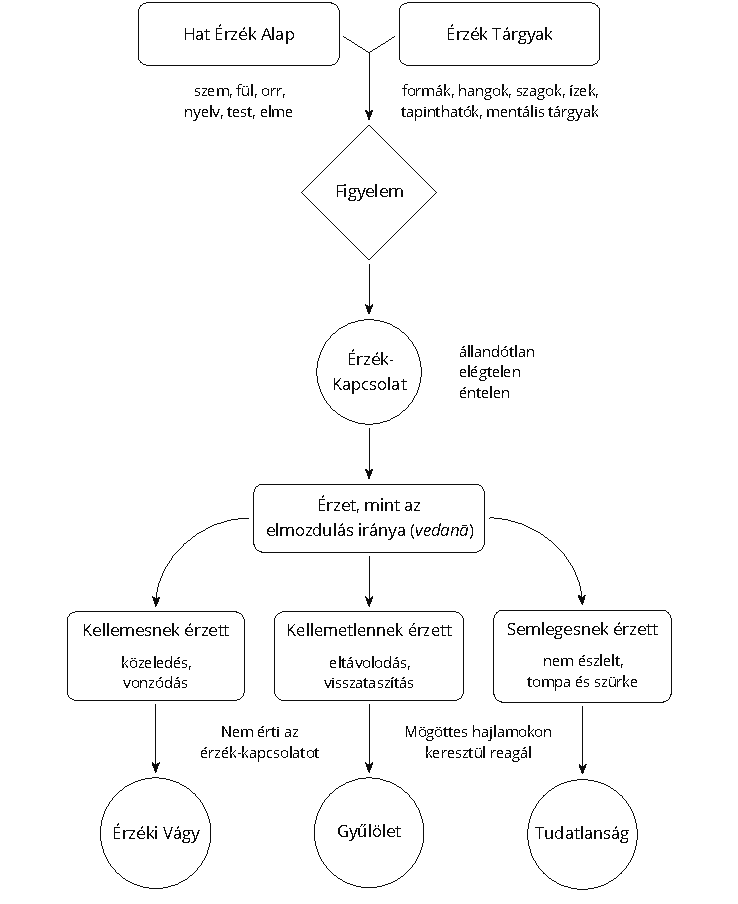
\includegraphics[width=\linewidth]{./manuscript/tex/diagrams/sense-contact-feeling-hu.pdf}
\end{figure}

\clearpage
\normalpagelayout

\vspace*{-\baselineskip}

\keywords{önnarratíva, elbeszélés}

Milyen hatással van ez arra, ahogy elbeszéljük magunknak a
tapasztalatainkat? Azt mondjuk magunknak, hogy ez az érzés jó volt vagy
rossz, és mit kellene erről gondolnunk. Egy központi eleme ennek a
narrátori szövegnek a \emph{mi érzéseink}, jellemzően abban az irányban,
hogyan legyen több a jó fajtából.

Mi történik, mikor észrevesszük, hogy mind a jó és a rossz tapasztalatok
instabilak, megbízhatatlanok, és a keletkezésük és elmúlásuk nincs az
irányításunk alatt? A belső értékeink átrendeződnek,
a vágy helyett a mulandóság által vezérelve.

\keywords{változékony természet, bölcs vizsgálódás}

Rendszerint akkor kezdünk csak figyelni, amikor észrevesszük, hogy
valami rossz, valami fáj, valami miatt szenvedünk. A kellemes
tapasztalatokra nem igénylünk annyi magyarázatot, ugye? Ezt a frusztrált
érzést, elégtelenséget és terjengő gondolkodást jelként használhatjuk a
magunk számára, hogy kezdjünk éberen vizsgálódni.

Gondolatban lépj egyet vissza, és figyeld a tapasztalatot mint egy
folyamatot, aminek van eleje, változáson megy keresztül, és megszűnik.
`A testben hol érzem ezt az érzést? Emlékszem, mikor kezdődött? Tudom
figyelni, ahogy változik? El tudom kapni, ahogy az érzés megszűnik?'

Nem tudjuk irányítani a világot magunk körül, de a hozzáállásunk
befolyásolja, mit látunk szabad választásként. A szemléletünk nyitja meg
vagy zárja be az ajtókat a tettek felé, amiket lehetségesnek látunk.
Ezek a tettek hozzák létre a helyzetet, amiben élünk, és befolyásolják,
ahogy a helyzetben látjuk magunkat. Ha nem vizsgáljuk a tapasztalataink
természetét, hajlamosak vagyunk a jó érzéseket jutalomnak és a rossz
érzéseket büntetésnek tekinteni, ennek folytán az életünk értelme ezek
körül fog forogni. A belső világunk mindig azokról a kérdésekről fog
szólni, mint: `Ki vagyok én \ldots{} Hogyan tegyem \ldots{} Miért kell
tegyem \ldots{} Mit kellene tennem \ldots{}' Nem olyan terhes érzés ez,
amit jobb lenne elhagyni?

Az alapos és felületes vizsgálat a \emph{szuttákban}\footnote{\href{https://a-buddha-ujja.hu/mn-2/hu/forizs-laszlo}{MN
  2}, Az összes káros folyamatról szóló tanítóbeszéd} használt
kifejezés, mely különbséget tesz a felületes figyelem között ami növeli
a zavarodottságunkat, és az alapos figyelem között ami tisztánlátáshoz
és helyes megértéshez vezet. A felületes vizsgálat átsiklik az
állandótlanság, elégtelenség és nem-én jellemzői felett, így mindent a
saját ügyének tekint. Az alapos vizsgálat felismeri az érzéki
tapasztalat jellemzőit, és a Négy Nemes Igazsággal összhangban
elmélkedik róluk.

\keywords{ragaszkodás az énhez, karóhoz kötött kutya, vizsgálódás}

Emlékszel, hogy egy kutya, pórázzal kikötve egy karóhoz, hogy futkos
körbe-körbe a karó körül? Ül, áll, járkál vagy futkos körülötte, de
minden amit tesz, a karó körül teszi.\footnote{\href{https://suttacentral.net/sn22.100}{SN
  22.100}, Póráz} Az ego által vezérelt gondolatok kavargása is ilyen.
Lehet, hogy elfoglaltan tart minket, de továbbra is ragaszkodunk a
középen lévő énhez, nem vagyunk képesek sehova máshova menni. A póráz az
azonosulás és megragadás (\emph{upādāna}), az a folyamat, ami kialakítja
az `én és enyém' képzetét az érzékek tapasztalatában, vagy akörül,
melynek alapvető igazság szerint nincs semmi ilyen jellemzője. Ez vezet
minket a felületes vizsgálathoz, arra összpontosítva kik vagyunk, mi
lesz velünk, növelve a kétségünket és zavarodottságunkat.

Az `én és enyém'-ben gyökerező kérdések csapdák. Egyre tovább
húznak-vonnak minket anélkül, hogy szabadsághoz vagy megálláshoz
vezetnének. Ha azt vesszük észre, hogy ki vagyunk kötve egy karóhoz, mit
tegyünk? Elvágni a pórázt jó ötletnek tűnik.

A meditáción belül értelmezve, a vizsgálódásra nem mindenféle
gondolkodás alkalmas. Nem minden fajta gondolat fog belátást
eredményezni. Vizsgálódó meditáció közben, a tapasztalatunkat ok-okozati
folyamatra bontjuk le, amire a Négy Nemes Igazságot\footnote{\href{https://a-buddha-ujja.hu/sn-56.11/hu/farkas-pal}{SN
  56.11}, A Tan kerekét forgásba hozó tanítóbeszéd} használjuk
útmutatóként.

Ez egy olyan tapasztalattal kezdődik, amit személyesen könnyű
azonosítanunk: a szenvedés, feszültség, elégtelenség, avagy Páli szóval
\emph{dukkha}. A gondolat iránya nem \emph{az én szenvedésem}, mint
személyes történet, hanem személytelen, természetes folyamatként
szemléljük azt.

\keywords{dukkha}

A kezdő álláspont azt elismerni, hogy a feszültség, a szenvedés
\emph{itt} van. Ez ismeretként triviális, hogy igen, van a világban
feszültség és szenvedés. De amikor magunk tapasztaljuk, szeretünk mégis
inkább valami másra figyelni, vagy hajlamosak vagyunk valakit hibáztatni
érte. Ezerféle dolgot teszünk, csak ne kelljen tudatosan elismerjük és
érdemben foglalkoznunk vele.

Az utasítás itt az, hogy csak az fog előre vezetni, ha a szenvedés felé
fordulunk, és azt vizsgálva keressük a megértés módját. A Buddha
tanításában ez az Első Nemes Igazság: van szenvedés, és a nemes
hozzáállás az, ha felé fordulunk és megértjük.

Mit értünk meg? Azt, hogy a szenvedés nem a semmiből jött létre, hanem
korábbi tényezők eredménye. Ha így tudjuk vizsgálni a helyzetet, nem
vagyunk tehetetlenek. Még ha nem is értjük a helyzetünk minden apró
tényezőjét, már az is megkönnyebbülés, hogy talán tudunk valamit
változtatni.

\keywords{a dukkha eredete}

A Második Nemes igazság arra mutat rá, hogy a szenvedést kiváltó okot
magunkban találjuk. Ez a kívánságunk, hogy a tapasztalataink másképpen
legyenek mint ahogy természetüktől fogva vannak. A görcsös
ragaszkodásunk ahhoz, ami állandótlan, törékeny, és nem megtartható. A
szenvedés, a \emph{dukkha} amit tapasztalunk, ettől a ragaszkodástól,
szomjas vágytól függ. Az utasítás, a nemes hozzáállás itt az, hogy ezt a
szomjas vágyat és ragaszkodást el kell engednünk, mert a mulandó
élményekhez való ragaszkodás szenvedés.

\keywords{a dukkha megszűnése}

A kiváltó ok megszűnésével megszűnik az eredmény, a szenvedés is. A jó
hír, hogy a szenvedés végét is magunkban találjuk.

Ebből a szemszögből láthatjuk, hogy az elme hozza létre azt a fajta
világot, amiben élünk. Ha figyeljük, van esélyünk, hogy legalább ne
rontsunk a helyzeten. És ki tudja, akár még javíthatunk is rajta?

A Harmadik Nemes Igazság erre irányítja a figyelmünket: van megoldás,
nem kötelező keserűségben és értelmetlen küszködésben élnünk. A tanács,
a nemes hozzáállás az, hogy gyakoroljunk és tapasztaljuk ezt meg a
magunk számára, a megértésen és a ragaszkodás elengedésén keresztül. Így
lehetővé tesszük a szenvedés megszűnését.

\clearpage

Még ha nem is tudjuk rögtön elengedni, már az is megkönnyebbülés, ha
látjuk az összefüggést: `Ha elengedném, nem szenvednék tőle'.
Ez már a munka fele. Egész eddig térkép nélkül bolyongtunk, de innen már
van út előre.

\keywords{a gyakorlás útja}

A Negyedik Nemes Igazság az út gyakorlását írja le. A Buddha nyolc
tényezőre bontotta, melyek magukban foglalják a mindennapi élet
helyzeteit és a meditáció fejlesztését is.

A Nyolcrétű Ösvény részei a (1) megértés, (2) szándék, (3) beszéd, (4)
tett, (5) megélhetés, (6) erőfeszítés, (7) éberség és (8) elmélyülés.
Amikor egy tényező összhangban van az igazsággal, \emph{helyesnek}
nevezzük: Helyes Megértés, Helyes Szándék, és így tovább. Az utat
részekre bontani segíti a vizsgálódást, könnyebb ilyen módon
gondolkodnunk, de az út tényezői nem különállóak: egymást erősítik és
támogatják. A gyakorlás egyesült egészként valósul meg.

Amikor leginkább szükségünk van a gyakorlásra, az \emph{azonnal} kell.
Nem állhatunk meg tényezőket számolni. Olyan eszköz hasznos, ami
hordozható és könnyen elérhető egy adott helyzetben. Mikor olvasunk,
töprengünk a jelentésen, van időnk körbejárni a szavakat, ez a tanulás
szakasza. Viszont az éber figyelem, mint elvont ötlet nem sokat használ
-- akkor értékes, ha gyakoroljuk, mikor kéznél van a jelen pillanatban.

\enlargethispage*{\baselineskip}

Mindig ide térünk vissza. Emlékszünk a múltra és tervezzük a jövőt, de
az emlékezés egy jelen tapasztalat, a tervezés egy jelen tapasztalat. A
meditáció gyakorlását nem a jövőért végezzük. Ha a megértést,
szabadságot, boldogságot, akadályok túllépését egy jövőbeli állapotként
látjuk, ezzel csak több lesz a terhünk. Az elengedés a jelenben
történik, ahol az állapotok nélkülünk változnak.

\clearpage

\section{Az Összes Káros Folyamatról (részlet)}

{\centering
\emph{\href{https://a-buddha-ujja.hu/mn-2/hu/forizs-laszlo}{MN 2}, Sabbāsava Sutta}
\par}

{
\setlength{\parindent}{0pt}\setlength{\parskip}{5pt}
\fontsize{9.5}{14}\selectfont

\emph{(A káros folyamatok megszüntetése az alapos figyelmen alapszik)}

Bizony mondom, szerzetesek, a káros folyamatok megszüntetése csak azok számára
lehetséges, akikben megvan a tudás és látnak; akikben viszont nincs meg a tudás
és nem látnak, azoknak nem lehetséges. Mit kell tudni és látni, szerzetesek, a
káros folyamatok megszüntetéséhez? Ez az alapos, mindenen keresztüllátó elme és
a nem alapos, nem mindenen keresztüllátó elme különbsége. Amikor a szerzetes nem
elmélkedik elég alaposan, új káros folyamatok keletkeznek, a már létrejöttek
pedig felerősödnek. Amikor a szerzetes alaposan elmélkedik, nem keletkeznek új
káros folyamatok, a már létrejöttek pedig eltűnnek.

\emph{(Aki nem ismeri a Tant, a nézetek sűrű bozótjába gabalyodik)}

Nem elég alaposan így elmélkedik:

`Léteztem én a múltban? Nem léteztem a múltban?'

`Mi voltam a múltban? Hogy léteztem a múltban? Abból, ami voltam, mivé lettem a múltban?'

`Létezni fogok a jövőben? Nem fogok létezni a jövőben?'

`Mi leszek a jövőben? Hogy fogok létezni a jövőben? Abból, ami voltam, mivé leszek a jövőben?'

Vagy most, a jelenben, kételyekkel a bensejében:

`Létezem én? Vagy nem létezem? Mi vagyok? Hogyan létezem? Honnan jött e lény? És hová tart?'

Mivel ezeket nem fontolja meg alaposan, e hat nézet valamelyike alakul ki benne:

`Van átmanom'\footnote{átman: `önmaga', az (ami mindig) önmaga (marad).} -- úgy alakul ki benne ez a nézet, mintha igaz és megalapozott lenne.

Vagy:
`Nincs átmanom' \ldots{}\\
`Az átmannal fogom fel az átmant' \ldots{}\\
`Az átmannal fogom fel a nem-átmant' \ldots{}\\
`A nem-átmannal fogom fel az átmant' \ldots{}\\
`Ez az átmanom, ami beszél és érez, ami mindenütt megtapasztalja a jó és a rossz tettek gyümölcsét – nos, ez az átmanom állandó, stabil, örökkétartó, nincs alávetve a szüntelen átalakulásnak, örökké ugyanaz marad'.

Ezt nevezik, szerzetesek, a nézetekbe gabalyodásnak, a nézetek sűrű bozótjának, a nézetek erdejének, a nézetek zavarának, a nézetek kínlódásának, a nézetek béklyójának. A nézetek béklyóival megkötözött, tanításban nem részesült, evilági ember nem szabadul meg a születéstől, öregedéstől és haláltól, a bánattól, a jajveszékeléstől, a fájdalomtól, a csüggedéstől és a kétségbeeséstől. Bizony mondom, nem szabadul meg a szenvedéstől.

\emph{(A nemes szívű tanítvány bölcsen elmélkedik)}

Bölcsen így elmélkedik:\\
`Ez a szenvedés';\\
`Ez a szenvedés keletkezése';\\
`Ez a szenvedés megszűnése';\\
`Ez a szenvedés megszűnéséhez vezető út'.

Amikor bölcsen így elmélkedik, a három béklyó -- az önvaló nézete, a kétely és a
vallási szertartásokhoz ragaszkodás -- megszűnik benne.

\clearpage

\emph{(Konklúzió)}

Szerzetesek, arról a szerzetesről, aki belátással \ldots{} megfékezéssel
\ldots{} használattal \ldots{} béketűréssel \ldots{} elkerüléssel \ldots{}
eltávolítással \ldots{} gyakorlással, megszabadult a káros folyamatoktól, --
arról a szerzetesről mondják, szerzetesek, hogy megszabadult az összes káros
folyamattól, megszüntette a sóvárgást, kioldozta a ragaszkodás béklyóit, és
tökéletesen átlátva az önteltségen véget vetett a szenvedésnek.

\bigskip

{\raggedleft
\emph{(ford. Fórizs László)}
\par}

}

\chapter{Ciklusok}

\keywords{lépések a gyakorlásban, leírások és tudatosság}

\noindent A meditáció a jelenbeli érzéseken, tapasztalatokon keresztüli
megismerést tanítja. Az utasítások lépésről-lépésre írják le a
fejlődést, de a jelenben csak egy pillanat elérhető számunkra. Előre
vagy hátra lépünk? Bármely irányban, a tapasztalat egyszerre egy lépés,
a lépés ahol minden változik. Szavakat használunk, hogy leírjuk a
tapasztalatot, de a tudatosság erre a tapasztalatra szótlan. Az éber
figyelem aktívan befelé néz, mintha önmagát kérdezné, de nem vár
választ. A nyelv szimbólumai is korlátozóak. Rögzített reprezentációkból
állnak, míg a tapasztalat mozgásban van.

A meditáció célja nem az utasítás lépéseinek tökéletesítése. A cél a
jelen tapasztalat tiszta ismerete, ami visszaállítja a helyes
nézőpontot. Kialakulhat bennünk az a benyomás, hogy mindig ugyanazt a
lépés sort kell teljesítenünk, és amikor az elme nem aszerint a sorrend
szerint fejlődik, csalódottak vagyunk.

\keywords{narrátor elme, tapasztalat mint alap, a megfelelő festéket választani}

És ami még rosszabb, úgy látszik mások békésen meditálnak, ők biztos jól
értik! A gyakorlás felszínre hozza az önkétséget. Vizsgálhatjuk ezt a
másik oldalról: Valaki talán dicsér minket, `Olyan békésnek tűntél, te
biztos tudsz valamit!' De mi tudjuk milyen szétszórt gondolatokkal volt
tele a fejünk, láthatjuk milyen megbízhatatlanok az ilyen benyomások.

A narrátor elme gépiesen folyton megjegyzéseket tesz, de nincs mögöttük
mélység vagy vizsgálódás. Érdemes egy lépés távolságból nézni ezt, és
megízlelni milyen megbízhatatlan és bizonytalan a saját gondolkodó
elménk, még ha azt is gondoljuk, `Ebben biztos vagyok!'

Fordítsd meg ezt a hozzáállást és kezdd a tapasztalattal. Egy kérdező,
kíváncsi figyelemmel indulj neki, ami szótlanul érdeklődik a jelenről.
Ha a tapasztalatunkat vesszük az alapnak, ahogy ez a tapasztalat most
van, az milyen megértést ad nekünk?

Először magunkat vesszük szemügyre -- Hogyan érezzük magunkat? Milyen
állapotban vagyunk? -- erre válaszolunk intelligensen, a meditációnk
megfelelő irányba való fejlesztésével. Amikor falat festünk, először a
falat vesszük szemügyre, kiválasztjuk az annak megfelelő festéket, és
\emph{azután} követjük az utasítást a dobozon. A rossz fajta festék le
fog peregni, nem igaz? Van amikor le kell higgadnunk, máskor energiát és
erőfeszítést kell bevetnünk, vagy várni, hogy a belső vihar tovább
álljon.

A meditáció különféle módszereinek lépései az imitáción keresztül való
tanulás része. Egy példát követve figyeljük önmagunkat és meglátjuk
hogyan működik az elménk. Amikor szenvedést érzünk, vagy fel tudjuk
oldani, vagy türelmesen kivárjuk, amíg véget ér. Később tiszta fejjel
visszanézünk, tudjuk mi történt minek a hatására, és a gyakorlásra
irányuló megértésünk nőni fog. Ebből tanultunk valamit, és nem
ragaszkodunk az első, bemutató példa részleteihez.

\keywords{fejlődés ciklusokban}

Ez egyszerű lenne, ha a meditációnk egyenes vonalban fejlődne, a
gyakorlással töltött percek és órák számával egyenes arányban. Azt
tervezzük, hogy le fogunk ülni, az elején kissé szétszórtan, de egy
órával később, \emph{ha jól tudunk meditálni}, nyugalmat fogunk érezni,
az elménk tiszta és összeszedett lesz. Legalábbis erre számítunk.

Később vissza emlékezünk mi történt a meditáció alatt, és azt látjuk,
hogy nem ez szokott történni. A tapasztalatunk nem egyenes vonalban
fejlődik a sekélytől a mélyig, vagy a szétszórttól az összeszedettig.
Azt gondolhatjuk, ez a mi hibánk, mert `nem vagyunk jók' a meditációban,
vagy `nem helyesen' követjük a lépéseket.

Amit megpróbálunk terv szerint, lépésről lépésre követni egy módszert,
minden az elvárásainktól eltérően történik. Arra gondolhatunk, `Talán
nem próbálom elég erősen?' Egyre jobban neki feszülünk, és egyre
fájdalmasabb lesz. Ilyen az az érzés, amikor egy véleményt rá akarunk
erőltetni a tapasztalatra.

Ha felidézzük, hogy a tapasztalatunk hogyan változik idő közben, más
mintát látunk. Egy tapasztalat megjelenik, változáson megy keresztül,
elmúlik, és egy újabb tapasztalat jelenik meg. Az elme ilyen ciklusokban
fejlődik, és ezek a ciklusok nem vesznek tudomást a céljainkról, hogy a
meditációnkat úgy akarjuk fejleszteni mint egy ranglétrát. A kommentáló
elme próbál egy személyes történetet illeszteni a tapasztalatra, arról,
hogy mi valaki olyan vagyunk, aki jó vagy rossz a meditációban.

Ehelyett vegyük a tapasztalatot alapigazságnak, és onnan induljunk.
Milyen fajta tapasztalat ez itt? Észrevehetjük, hogyan mozog a figyelem,
mint a tudatosság egy folyamata, hogyan megy keresztül különféle
ciklusokon.

Eleinte az elme elégedett az üléssel, ellazult figyelemmel pihen, mint
amikor egy séta után leülünk egy padra: ülni és lélegezni a béke
teljessége. De gondolatok jelennek meg és követjük őket. Megállunk, újra
nyugodtak és csendesek vagyunk, a gondolkodás lehet, hogy meg is áll
anélkül, hogy észrevennénk, hogy nem gondolkodunk. De a figyelem elkezd
mozogni, és megint észrevesszük magunkat, hogy gondolkodunk. Emlékek,
vágyak, nyugtalanság jelenik meg és észrevesszük, hogy ezen dolgoznunk
kell. Ezután az elme újra nyugodt, és visszatér a csendesség érzéséghez.

\keywords{tudás és megismerés, névadó folyamat, a tudás nem a miénk}

Némi ismeretre szükség van, de egy kevés is elég. A Buddha tanítására
emlékezni olyan kincs, ami nem fogy ki. A belátások és megértés viszont
nem válik a \emph{mi tudásunkká}, mintha az attól fogva a tulajdonunk
lenne. Az igazságot nem tehetjük egy dobozba, hogy eltárazzuk a
következő alkalomra, ehelyett folyamatosan felismerjük azt a jelenben.
Amikor rögzített elképzeléseket hozunk létre arról, amiről úgy gondoljuk
ezt már tudjuk, a gyakorlásunk elveszíti a kapcsolatot a valósággal.
Minden alkalommal újból az elejénél kezdjük, és onnan, bízunk a jelen
megismerésében.

A gondolkodó elme vonzódik a tényekhez és megállapításokhoz, egyfajta
biztonságot érzünk abban, ha tényeket tudunk felmondani. Szeretnénk
megállapítani, hogy `ez jó meditáció volt, ez rossz meditáció volt'.
Különbséget akarunk tenni és nevet adni a tapasztalatnak.

Ilyen az elégedetlen elme. Valamivé válni akar, meg akar érkezni egy
állapotba és nevet akar magának. De sehol nem szeret megállni. Megy
tovább és tovább, amíg csak észre nem vesszük, hogy a folytonos futásban
teljesen kimerültünk.

Amikor a tudatban láthatóvá válik, hogy mi magunk tesszük ezt, a
névkeresés megáll. Megáll, mert a látás felváltotta a nem-látást; a
tudás felváltotta a tudatlanságot. Tudatosan látni a névadó folyamatot
elegendő, hogy megtörje a kényszert a folytatásra.

A jelenben minden változik, semmi sem rögzített. Minden mozog, a
tapasztalat erre-arra fordul és folyik. Nem áll meg egy fotóra és vár
amíg nevet adunk neki. Ebben a változásban, a kétséggel és aggodalommal
teli kérdések, az önazonosság és a célok elvesztik a jelentésüket. A
\emph{Mahāsatipaṭṭhāna Szutta} kifejezését használva: `\emph{Szabadon
időzik, semmihez sem kötődve a világon}.'\footnote{\href{https://a-buddha-ujja.hu/mn-10/hu/toth-zsuzsanna}{MN
  10}, Az éberség megalapozásáról szóló tanítóbeszéd}

Ennyi elég, így ismerve az elmét megállunk és megérkezünk egy helyre,
ahol hálásak tudunk lenni a létezésért. Nem egy különös dolog miatt.
Hálásnak lenni, hogy van tapasztalat, megismerés, tisztánlátás, és a
szabadság, ami engedi, hogy megálljunk és nem kell több és több felé
mennünk.

\keywords{határozatlan vonalak, korlátozott szimbólumok, megismerés névadás nélkül, érzések határvonalak nélkül}

Kiegyensúlyozott testtartásban a test kifinomult belső érzéseit könnyebb
megfigyelni. Befelé irányítjuk a figyelmet, kíváncsi hozzáállással. Nem
tudjuk előre mit fogunk találni.

Megjelennek a test érzetei, illetve az érzések, amik a megismerésükhöz
társulnak. Megtapasztaljuk őket, de gyakran nincsenek tiszta
határvonalaik. Nincsenek éleik, vagy határozott formájuk. Próbálunk
szavakat találni rájuk, de ezek nem illeszkednek jól. Nem vagyunk
biztosak abban, hogy minek nevezzük őket.

\enlargethispage*{\baselineskip}

Minden szimbólum, amit névként használhatnánk, hiányos. A nyugati
kultúránkban erősen bízunk a tényekben, és szeretünk visszatérni ahhoz a
biztonsághoz, amit a nevekben és terminológiában érzünk. Nem ismerősek
számunkra azok a tudati folyamatok, amik nem használnak neveket és
rögzített szimbólumokat. A megfigyelt érzések, a tapasztalat maga nem
tisztán meghatározott, de mégis tudjuk, hogy jelen van ez a tapasztalat.

Így meg tudjuk különböztetni a nevet adó folyamatot magától a
tapasztalattól. A test kifinomult érzései ködszerűek, nincsenek éles
határaik. Belégzés és kilégzés közben, megtapasztalhatjuk milyen ez az
érzés az egész testben -- mindenhol egyszerre. Az egész test lélegzik.
Van érzés és tapasztalat, de nincsenek nevek és éles határok.

A nevet adó folyamatot elhagyjuk, és észre vesszük, hogy képesek vagyunk
ismerni ezeket az érzéseket, ahogy jelen vannak. A megismerő elme örömét
találja abban, hogy szűrők nélkül szélesebb körben fogja be a
tapasztalatot. Tudjuk, hogy milyen a tapasztalat, anélkül, hogy nevet
kellene találnunk rá.

\keywords{az elme vizsgálata, túl sok gondolkodás}

A kártékony elmeállapotok érzetében észrevehetünk egyfajta hőséget,
nyugtalanságot, elégedetlenséget és szorongást. Emlékezünk, hogy
türelemmel forduljuk felé, és fenntartsuk a kitartást az állapot
érzéseinek jelenlétében. Ez is meg fog változni, ez is el fog múlni, és
meg tudjuk ezt várni. Amikor tudjuk hol állunk, a legtöbb esetben ennyi
elég. Az elme folyamatai maguktól meg fognak változni. Ha nem teszünk
tüzelőt a tűzre, az el fogja égetni amije van és magától kialszik.

Az elhatározás és ismétlés része a gyakorlásnak, de egy kifejezett cél
felé törekedésben az erőfeszítés keserűvé és fárasztóvá válik. `Ez már a
teljes felébredés? Vagy legalább egy része? Mikor fog már szólni a
meditációs harang?' Ne~egy állapotot keress. Az elme, ami felébredetté
akar válni, túlbonyolítja a helyzetet.

A jelen tapasztalat mindig egyszerű, az éber figyelemnek megvan a
képessége a bölcs megértésre. A gyakorlásban folyton ehhez térünk
vissza, ez irányítja az erőfeszítést.

Ezt nem erőltethetjük akarattal, és nem garantálhatjuk mi fog történni:
bíznunk kell a folyamatban. Ami marad, az a jótékony elme ami érti mi
történik. Nem sürget minket a kényszer, és nem kell végig erőltetnünk
magunkat a dolgokon. A nehézség után van terünk ahhoz, hogy megjelenjen
a hála, és értékelni tudjuk a könnyedség hűs, kényelmes érzését.

\keywords{beépített gyakorlás}

A tanítóinkra nézünk fel példaként. Nem azért meditáltak, hogy elérjenek
egy különleges állapotot és azután keressenek valami más tennivalót. A
meditáció nem elkülönült, hanem beépült az életükbe. A \emph{szutták}, a
buddhista hagyomány megőrzött szövegeinek példáiban, a Tiszteletreméltó
Száriputta az üresség szemléletét gyakorolta,\footnote{\href{https://a-buddha-ujja.hu/mn-151/hu/fenyvesi-robert}{MN
  151}, Az alamizsna megtisztítása} míg a Buddha a jeltelenre irányuló
koncentrációt tartotta fenn. Így folytatták a meditációt.

\chapter{Csónak}

\keywords{sétáló meditáció módszere}

\noindent A sétáló meditáció egy energikusabb alternatíva az ülő
testtartás mellett. Keress egy ösvényt, vagy egy kis területet, ahol van
elég hely megtenni néhány lépést, oda-vissza séta közben. Habár
sétálunk, a figyelmünket befelé irányítjuk. Nem egy bizonyos helyre
sétálunk. A sétáló testtartást használjuk az elme fejlesztésére.

Egy kültéri, magányos helyszín az ideális, de beltérben, egy nagyobb
szoba is megfelelő.

Válassz két pontot, ami között tisztán járható út van. Ez lehet két fa,
vagy akár két bútor is. Egy rövid ösvény vehető tizenöt lépés hosszúnak,
egy hosszabb lehet harminc lépés is. Állj meg az ösvény egyik végén, és
indulj el lépésenként, figyelmesen a másik végéhez, tisztán elhatározott
szándékkal arra, hogy a meditáció tárgyával maradsz, mint például a
lélegzet, vagy a mozgó test fizikai érzetei. Irányítsd a tekinteted
lefelé, nézz magad elé néhány lépésnyire. Az ösvény másik végén állj
meg, és várj pár lélegzet vételnyi időt. Tartsd a figyelmed elmélyedve a
meditációban, fordulj meg, és kezdj el sétálni a másik irányba.

Tartsd a kezed úgy, hogy segítsen fenntartani a folyamatos belső
figyelmet. A legtöbben összefogják a két kezet maguk előtt. Nem a kezek
pontos helyzete számít, de ha oda-vissza lengeted a karjaid, az könnyen
eltereli a figyelmed.

\clearpage
\thispagestyle{empty}\mbox{}
\photoFullBleedPlaceholder{%
  TODO: Illustration of walking meditation.%
  \illustration{Sétáló Meditáció Testtartás}%
  \label{illus-walking-meditation}%
}
\clearpage

Igazítsd a séta sebességét az energia szintedhez és a meditáció
tárgyához. Egyesek gyors és határozott lépésekkel gyakorolják a sétáló
meditációt, mások lassú és óvatos lépéseket tesznek. A megfelelő
sebesség akár egy alkalom időtartamán belül is változhat. Tapasztald meg
a különféle változatokat és találd meg azt, ami illeszkedik a
gyakorlásodhoz és mentális hátteredhez az adott helyben és időben.

\keywords{az érzések manipulálása, fontoskodás}

Korábban, a sétáló meditációtól csak még feszültebb lettem. Úgy
gondoltam hasznos, de a módszer elég határozatlan volt, és nem voltak
pontos részletek arról, hogyan is kellene azt végezni. Úgy éreztem, egy
pontokba szedett listára van szükségem, amin végig mehetek és
ellenőrizhetem, jól végzem-e a feladatot vagy sem.

Folyton el akartam sétálni egy \emph{másik helyre}, ahol majd
\emph{máshogy érzem} magam. Elkezdtem a sétáló meditációt két fa között,
de úgy éreztem mintha nem lenne semmi hatása, és folyton változtattam a
séta módját, hogy manipulálni tudjam hogyan érzem magam. `Lépkedj
gyorsabban, az használni fog. Lassíts le, és összpontosíts. Próbálj így
lélegezni, és úgy lépkedni, amíg máshogy nem érzed magad.'

Az is fontos volt, hogy mások lássák, valami fontos dolgot csinálok.
Addig járkáltam oda-vissza, amíg a füvön elkezdett látszódni a
kitaposott ösvényem. Ez volt a bizonyíték: 'Itt van, látom, hogy tettem
valamit, és \emph{mások} is láthatják!

Látható, hogy az ilyen küszködést mennyire az a kérdés vezérli: `Hogyan
tudnám jobban érezni magam, magammal kapcsolatban?'

A motiváció az érzések \emph{manipulálása} körül forog, nem azok
\emph{megértését} keresi, hogyan keletkeznek és múlnak el. A fontoskodás
nem hasznos hozzáállás a gyakorláshoz. A vágyunk meghatároz egy külső
jelet, és szörnyen fontossá válik, hogy ezt lássuk, és, hogy mások
számára látható legyen. Az a \emph{fontos} ösvény a fűben amit a fűbe
tapostam (ami valószínűleg eltűnt a következő reggelre) egy példa erre.
Kifejezni ezt a magunk számára, amikor észrevesszük, hogy ez történik,
már önmagában megváltoztatja a hozzáállásunkat a folyamathoz.

Egy hasznos hozzáállás a gyakorláshoz az, ha úgy közelítjük meg, mintha
valami teljesen hétköznapi dolgot végeznénk, de ehhez hozzáfűzzük a
felfedezés szemléletét, és emlékezünk arra, hogy az értéke nem egy
világi cél, ebben nincs tét, amit megnyerjünk, vagy elveszítsünk. Az is
segíthet, ha \emph{csökkentjük} a meditáció idejét. Jó benyomást kelt,
ha három óra hosszat folyamatosan sétáló meditációval töltünk, de a
nyomás feszültséghez vezet. Mi a helyzet tíz perc meditációval? Lehet,
hogy nem világhír, de talán jó élmény és érdekes lesz.

\keywords{gondolatok megállítása, éberség a fejben, belső monológ, irányítás, hétköznapi gyakorlás}

A gondolkodás jellemzően erősödik és önmagunk körül forog, amikor úgy
tekintünk az éberségre, tudatosságra, vagy a meditációra, mint egy olyan
dologra, ami valahol a fejünkben történik. Abból a nézőpontból, az
éberség olyan dologgá válik, amit `nekem kell csinálnom az
agyamban'.\footnote{Cf. Chapter 4, `Mindfulness Mania' in
  \href{https://www.goodreads.com/book/show/44439993-why-i-am-not-a-buddhist}{Why
  I Am Not a Buddhist by Evan Thompson}} Ez alá becsüli az éberséget,
mintha csupán egy rongybaba lenne az agy bábszínházában. Habár ez a kép
illik a kedvenc elképzelésünkhöz, ami szerint mi irányítjuk a műsort, ez
a valóság egy szűk nézete.

A kognitív felfogásunk ennél egy sokkal összetettebb, a környezetet
magába foglaló folyamatok rendszere. Megfigyelheted, hogyan változik a
figyelmed, vagy az egész személyes hozzáállásod, például amikor egyik
épületből belépsz a másikba, vagy a belső térből a szabadba. A tested
reagál arra, hogy egy új környezetben vagy, a különféle szociális
környezet megváltoztatja a viselkedésed, nagyszámú belső és külső
tényezők vesznek részt abban, hogy létrehozzák az észlelést, amit úgy
tapasztalsz mint `az én elmém.' A felfogásunk, vagy elménk, magába
foglal egy hálózatban működő folyamatok együttesen működő rendszerét,
melyek a testünk széles környezetéből veszik a beérkező jeleket. Ahogy
többet tapasztalunk ebből történés közben, az derül ki, hogy nincsenek a
kezünkben a drótok, amiket meghúzva az elménk akaratunk szerint járja a
táncot.

A gondolkodó és érvelő elme egy eszköz, amit a minket motiváló célokra
használunk. Nem a `jó érv' motivál minket, hanem a motiváció miatt
keresünk jó érvet. Ne akarj a gondolatok végére jutni; vedd észre mi az,
ami motivál téged a gondolkodásra. Ha azt elengeded, a gondolkodást is
elengeded. A belső rágódással gyakran magunkat akarjuk vigasztalni úgy,
hogy elképzeljük, mintha lenne irányításunk egy bizonyos helyzetben;
vagy megpróbáljuk visszanyerni az irányítást valami olyasmi felett, ami
már megtörtént. Olyan ez, mintha az esőről gondolkodnánk: esni fog attól
függetlenül, hogy rágódunk rajta vagy sem.

Ha \emph{tudunk} tenni valami hasznosat a problémával kapcsolatban, az
megnyugtató. Ha nem tudunk, mert teljesen az irányításunkon kívül esik,
legalább ezt tudhatjuk, és felhagyhatunk a belső tépődéssel.

A gondolkodásnak gyakran egy élesen meghatározott szóbeli tárgya van.
Amikor a figyelmünk módját eltoljuk egy tágasabb, folyékonyabb
hozzáállás felé, az elme nem tud szavakat találni rá, és átváltunk egy
nem verbális, szótlan felfogási módba; a körülöttünk lévő világot ezen
keresztül észleljük.

A nem-gondolkodás úgy tűnhet mint valami misztikus állapot, mintha egy
magas fokú meditációs szint lenne. Nem szoktuk megkérdezni meditáló
társainktól mennyi belső párbeszédet használnak, ugye? Amikor
megkérdezzük az embereket, kiderül, hogy van aki egyáltalán nem folytat
magával belső monológot.\footnote{\href{https://www.psychologytoday.com/us/blog/pristine-inner-experience/201110/not-everyone-conducts-inner-speech}{Not
  Everyone Conducts Inner Speech (psychologytoday.com)}} Sokkoló
meglepetésként éri őket, amikor megtudják, hogy más emberek beszélnek
magukkal a fejükben. Mások csak időnként kezdenek belső párbeszédet, míg
megint mások folyamatosan, szünet nélkül ezt teszik. Ez egy érték skála,
mint egy tekerő gomb különféle állapotai. Személyesen hozzá vagyunk
szokva egy bizonyos mértékű belső párbeszédhez, de a szint, amin ezt a
mentális képességet használjuk egy szokás, amin állítani tudunk.

Ha séta közben úgy érzed, magával ragadott a gondolkodás, vedd tágabbra
a területet, amire tudatos vagy; hogy magába foglaljon egy szélesebb
kognitív mezőt. Idézd fel a nyugodt hallgatás hozzáállását, fordítsd el
a figyelmet a szemek és a fej környékéről más irányba.\footnote{Cf. page
  117, Gently Listening in
  \href{https://forestsangha.org/teachings/books/alert-to-the-needs-of-the-journey?language=English}{Alert
  to the Needs of the Journey by Ajahn Munindo (forestsangha.org)}}
Tartsd a szemeket magad előtt, alacsonyan a sétáló ösvényen.
Képzelheted, mintha minden irányba látnál a testeddel, vagy mintha az
ösvényt a talpaidon keresztül látnád, a tapintás és nyomás érzetein át.
Nyisd meg a figyelmed, hogy magába foglalja az egész testet, mint
egyetlen mozgásban lévő érzet. Nyisd a figyelmet még tovább, ki a sétáló
ösvény közvetlen környezetére.

Rövid meditációk, amik betöltik a céljukat, jobbak, mint hosszú
időszakok, amit azzal töltesz, hogy az óra állásán aggódsz. A cél nem
az, hogy több feszültséget keltsünk. A cél az elme tisztán látása és
nyugalma. Gyakorolunk, vele maradunk, így élünk abban a térben, ahol a
feszültség feloldódik.

\keywords{a tapasztalatok figyelése, érzékek kontaktusa}

A meditáció elején összegyűjtjük a figyelmünket azzal, hogy a légzést
figyeljük, vagy a séta közben tapasztalt érzéseket, lépésről lépésre.
Egy zaklatott, izgatott elmétől nem várhatunk éber és kiegyensúlyozott
intelligenciát, ezért lényeges megalapozni legalább némi nyugalmat.

Vizsgálódásra a nyugodt elme alkalmas. Mit tanulhat a boldog ember a
Buddha tanításából? Mit tanulhat a boldogtalan ember? Vagy, aki nem érzi
magát sem különösen jól vagy rosszul, éppen megvan ahogy van?

A tapasztalatunkat figyeljük, az állandótlanság jeleit, az érzések,
gondolatok kezdetét és végét, ahogy megjelennek, változnak és
megszűnnek. A magunk számára vizsgálódunk, ez ad a tanítások szavainak
jelentést és közvetlen hasznot.

Tapasztalataink az érzékeken keresztül nyilvánulnak meg. A szem formákat
és színeket fog fel, a fül hangokat, az orr szagokat, a nyelv ízeket, a
test a tapintás, a hideg és meleg benyomásait érzékeli, az elme pedig
észleli a gondolatokat, emlékeket és más mentális folyamatokat.

\keywords{három érzés, állandótlanság}

Az érzetek (\emph{vedanā}) három minőségben jelennek meg. Lehetnek
kellemesek, és vonzódunk feléjük; lehetnek kellemetlenek vagy
fájdalmasak, és inkább távolodnánk tőlük; vagy lehetnek semlegesek, és a
jelenlétük nem zavar minket. A semleges érzetek egy jellemzője, hogy
kellemessé válnak, ha figyelünk rájuk, mint a légzés.

A megjelenésük és elmúlásuk nincs közvetlen irányításunk alatt. Az érzet
szükséges feltételei a kapcsolat az érzék és érzék-tárgy között,
illetve, hogy a figyelmünk oda irányuljon. A kapcsolattal az érzet
magától megjelenik. Amikor a érzék-kapcsolat megszakad, vagy a
figyelmünk másfelé fordul, az érzet megszűnik.

A boldog ember, aki kellemes érzéseket tapasztal, tanulhat ezek
vizsgálatából. A vonzó benyomás arra vezeti minket, hogy ragaszkodjunk a
kellemes érzethez, ha elfelejtjük, hogy ez a függő állapot
megbízhatatlan. Az érzeteket nem birtokoljuk. Lehetetlen megtartani,
nincs mélyebb lényege, `én' nélküli, üres.

\enlargethispage*{\baselineskip}

A boldogtalan ember, aki kellemetlen, fájdalmas érzéseket tapasztal, azt
tanulhatja, hogy ez az állapot nem lesz maradandó. Láthatjuk, hogy
fölösleges ezen felhúzni magunkat haraggal vagy gyűlölettel. Mikor
tettre van szükség, cselekszünk, mikor türelemmel várnunk elegendő,
várunk.

Aki úgy érzi, semleges és szürke világban él, elkerülheti, hogy
elsodorja a figyelmetlenség és ködös zavarodottság. Ez a semleges
állapot sem lesz állandó, és ha az éberség hiányában téves nézetet
követ, az eredmény fájdalmas és veszélyes lehet, mintha a ködben falnak
rohannánk vagy gödörbe esnénk.

Az állandótlanság és üresség alapvetően megváltoztatja a nézőpontunkat,
átrendezi az értékeinket.

A Buddha úgy jellemezte az érzeteket, hogy `az érzetben találkozik
minden dolog.' A szem formákat lát, a fül hangokat hall, a test
tárgyakat tapint, és így tovább. Az érzék-alap kapcsolatba kerül az
érzék-tárggyal. Ha ott van figyelem, van kapcsolat, és az eredmény az
érzet.

Az érzetek magukhoz vonzzák a figyelmünket, mint egy mágnes.
Emlékezhetünk a szuttákban található lépésekre:

\begin{quote}
A vágyban gyökerezik minden dolog.\\
A figyelemből születik minden dolog.\\
A kapcsolatban jelenik meg minden dolog.\\
Az érzetben találkozik minden dolog.

\bigskip

\quoteRef{%

\href{https://suttacentral.net/an10.58}{AN 10.58}, Gyökerek

}
\end{quote}

\keywords{érzetek éntelen jellege, érzetek mint buborékok, haraggal megbirkózni}

Ezen a ponton tesszük bonyolulttá a dolgot. Ha úgy látjuk, mint egy
átmeneti, megbízhatatlan jelenség, nem csinálunk belőle problémát. Nem
kezdünk hozzá ragaszkodni, a szomjas sóvárgásnak nincs alapja, amiből
keletkezzen, és nem válunk feszültté. A Buddha az érzeteket a
buborékokhoz hasonlította, amik erős esőzés közben megjelennek a víz
felszínén.\footnote{\href{https://suttacentral.net/sn22.95}{SN 22.95},
  Egy Darab Hab} Gyorsan megjelennek, majd eltűnnek. Hogyan lehetne
bármi is egy buborékban, amit meg tudunk ragadni?

Azonban a bevett szokásunk, hogy feltesszük, hogy ez az érzet `én'
vagyok, vagy az `enyém'. Ebből megszületik a szomjas sóvárgás, akár úgy,
mint a vágy arra, hogy többet kapjunk belőle, vagy arra, hogy
megszüntessük. Miközben azzal töltjük az időnket, hogy vonzódással és
eltaszítással reagálunk, a mögöttes, kényszeres hajlamokat (érzéki vágy,
gyűlölet és tévhit, a három \emph{āsava}) tápláljuk, és ezek egyre
erősödnek az elmében.

Úgy látszik, sok mindent rendbe kell tegyünk az elmében, de megéri. A
haraggal megbirkózni, például, a gyakorlás egy kifejezetten eredményes
része. Ez egy könnyen felismerhető elme állapot, és így könnyen célba
vehető. Még egy kis mértékű haladás is belső megértést ad számunkra
magunkról, és arról, hogyan működik a buddhista gyakorlás. A harag
hatásai fájdalmasak, betegnek érezzük magunkat, elvesztjük az
intelligenciánkat, és pusztítóan hat mind a személyes és szakmai
kapcsolatainkra. A mohóság rendszerint ragadós, tudjuk, hogy nem
kellene, de még is akarjuk; a tévhitben elveszítjük az irányt; a
félelemhez félünk túl közel kerülni; de könnyű azt akarni, hogy ne
legyünk dühösek. Szabadnak lenni a haragtól egy megkönnyebbülés, és a
haladás minden lépése könnyebbé teszi a következő lépést. Amint egyszer
lehűlik a fejünk, ami marad, az önbecsülés érzése, és a gyakorlásra való
elhatározás.

\clearpage

\keywords{félelem és szorongás}

Ha veszély van, vagy a helyzetünk bizonytalan, természetes, hogy arról
gondolkodunk mit kellene tennünk, a félelem és szorongás érzése meg fog
jelenni, mert jó ok van rá. A félelem, mint érzelem, a lehetséges
veszély információját hordozza, a szorongás, mint érzelem, egy
bizonytalan eredményt foglal magában. A félelem óvatossá tesz minket,
ami hasznos -- nem szeretnék egy autóban ülni olyan sofőrrel, aki nem
fél az ütközéstől.

Mit várhatunk el a meditációtól? Azt gondolhatjuk, \emph{ha jól tudnánk
meditálni}, meg tudnánk állítani a félelmet és szorongást. Ha
alkalmaznánk a megfelelő technikát vagy felidéznénk a megfelelő
szavakat, ezek az idegesítő elme állapotok eltűnnének. Vedd észre ebben
a motivációban az irányításra törekvő vágyat. Azt kívánjuk, hogy a
helyzetünk más legyen, mint amilyen, láthatjuk a vágyat ami manipulálni
és megszüntetni akarja.

A hozzáállásunk befolyásolja milyen irányba fejlődik az érzés. Annyi
biztos, hogy ronthatunk rajta. Egész idő alatt, magunkban vitatkozunk
magunkkal, elképzeljük, ahogy a helyzet ilyen vagy olyan módon
lejátszódik. A szorongást követő belső párbeszéd a körülöttünk történő
események irányítására törekvés egy formája. Újra-értelmezni próbáljuk
amit látunk olyan módon, ami illeszkedik a helyzetről alkotott korábbi
nézetünkhöz. Amikor az érzés már megjelent, nem tudjuk megváltoztatni
vagy kijavítani, de továbbra is részünk van a folyamatban. Az elmére
való tudatosság biztonságos keretben tartja, de teret ad neki, hogy
kifussa magát és véget érjen.

Amikor a reptéren a csomagomra várok, érzem a szorongást -- vajon
elvesztették a csomagom? Megtettem mindent amit tennem kellett, és most
semmit többet nem tehetek. Érzem a szorongást, mert a csomagom helyzete
valóban bizonytalan. A gyakorlás részeként felidézem, hogy tudok helyet
adni ennek az érzésnek és vele maradni, nem kell siettetni, addig
maradhat ameddig maradnia kell.

Nem tudjuk megállítani, de megállhatjuk, hogy rontsunk rajta. Ha veszély
van, megtesszük ami szükséges. Ha pillanatnyilag nincs veszély, de
szorongást érzünk, felismerhetjük, hogy \emph{nem a szorongás a
veszély}, és éberen jelen maradunk, az érzéstől való félelem nélkül.

\keywords{a test vizsgálata, egyszerűsíteni a módszeren, csillapítani a gondolkodást, BUD-DHÓ}

Hogyan észlelhetőek számunkra az érzetek, a testen keresztül szemlélve?
Hol érezzük? Mikor kezdődött? Változásban van? Valóban olyan rossz, mint
testen belüli érzet? Az ilyen vizsgálat ugyan nem ad nekünk irányítást,
de fejleszti a megértést, hogy az érzet nem jelent veszélyt, és nem kell
folytatnunk a belső küzdelmet az irányításért.

Ha a gondolatok nem csillapodnak, lefoglalhatjuk a gondolkodást egy
előre eldöntött gondolattal, ahelyett, hogy engednénk minden irányba
rohanni. A BUD-DHÓ mantra hasznos ilyenkor. Ez egy egyszerű módszer, ami
összefogja a szétszórt figyelmet, és alkalmassá teszi, hogy a mi
hasznunkra dolgozzon.

Ha úgy érzed a meditáció túl bonyolult, egyszerűsítsd le a lényegre. A
sok bonyolult lépéstől csak növekszik az ismeretlenség és kétség érzése.

Egy lélegzet, egy BUD-DHÓ. Belégzés közben magunkban szavaljuk a mantra
első felét, BUD-. Középen a lélegzet megáll egy pillanatra. Kilégzés
közben a másik felét szavaljuk, -DHÓ. BUD-DHÓ.

A lényeg a megértés, ami megállít, és békét hagy maga után ott, ahol
`te' voltál. A béke abból ered, hogy az érzékek visszahúzódnak, és a
figyelem folyása befelé fordul. A keresés megáll, mert ami van az elég,
sehova nem kell mennünk.

\keywords{szomorúság az ürességben}

Az első benyomásunk az ürességről lehet, hogy a veszteségre irányul, és
szomorúságot kelt bennünk. Több tapasztalattal megtanuljuk felismerni az
üresség kifinomultabb oldalait, amiben nem birtoklunk, de nem is
vesztettünk el semmit: ez az üresség felszabadító.

Amikor a világi célokról kiderül, hogy üresek, és nem olyan fontosak
mint az gondoltuk, ez szomorúságot és irányvesztést okozhat, nem vagyunk
többé biztosak abban, merre tartsunk.

Olyan ez, mint mikor ébredés után nem vagyunk biztosak magunkban, egy új
világ veszi át az álom helyét. Miután a zavar elmúlik, csendes öröm
jelenik meg az elmében. A folyamatos éberség felismeri a jelenben lévő
boldogságot. Az értékek átrendeződnek, nem kívül keressük az erőt és
biztonságot, mert a függő feltételek bizonytalanok, elégtelenek, és a
vég nélküli hajszolásuk kimerítő.

Ki az, aki szenved? Ez a tapasztalat, hogyan változik? Hol van a béke
most? Hol van a megértés most? A tapasztalat nem egy megoldani való
probléma. A tudatos figyelem vele marad és felfogja.

\enlargethispage*{\baselineskip}

Fordítsd a figyelmet a kérdés előtti pillanatra: ki kérdez kit? Ez a
narrátori elme trükkje, elképzel valakit, akihez beszél, valakit akit
kritizál vagy panaszkodik neki, de a mikrofonba beszélő hang és a
hallgató ugyanaz, és a kérdés és válasz között egyik sincs: csak a
figyelem.

\clearpage

\keywords{a világ történetei, BUD-DHÓ}

BUD-DHÓ, belégzés, kilégzés: a világ történetei nem érdekesek számunkra.
Amikor a kérdező figyelem megállítja a szavakat az elmében, ennyi elég.
Hallgató figyelem tölti be a szünetet, és a válasz a jelen tapasztalat.

A lélegzetre és a BUD-DHÓ mantrára épülő meditációt könnyű informális
helyzetekhez is igazítani. Hétköznapi helyzetben, akár egy mantrával,
akár szótlanul is, egyszerűsítsd le a gyakorlást, amíg a megfelelő
hozzáállást tisztán látod. A légzés figyelése egy egyszerű gyakorlat,
ami nem add több bonyodalmat a világi jövés-menéshez. Nem kell
megoldanod a tapasztalatot, elég figyelni és hallgatni.

\keywords{tudong történet, ön-kritika, ön-támogatás, az ellenszenv eltorzítja a Dhammát}

Egyszer egy sétán voltam, kinn a vidéki utakon. Egyik falutól a másikig
vándoroltam egy hátizsákkal, egy kis sátorban aludtam, és minden nap
betértem a legközelebbi faluba abban a reményben, hogy talán kapok némi
ételt aznapra. Ezt a gyakorlatot \emph{tudong}-nak nevezzük. Térképeket
nyomtattam A4-es lapokra, ezekre rendszerint jegyzeteket is írtam. Ekkor
már néhány napja úton voltam, a papíron jelezve milyen utakat követtem;
megjelölve ahol jó sátrazó helyeket találtam; jegyezve hol kaptam
alamizsnát a faluban; és így tovább. Olyan ez, mint egy útinapló. Mikor
visszaérek a kolostorba, be szoktam szkennelni a térképeket és legépelem
a jegyzeteket.

\enlargethispage*{\baselineskip}

Egy esős és szeles napon, éppen egy sáros úton jártam, kinn a semmi
közepén. Leültem pihenni, és gondoltam, bejelölöm ezt az útszakaszt a
térképen. Megnéztem a műanyag tasakot ahol a térképeket tartottam, és
láttam a mai térképet, de a tegnapi nem volt ott. \emph{Elvesztettem a
tegnapi térképet.} Minden feljegyzéssel együtt.

Biztosan kiesett valahol korábban, amikor kivettem megnézni a mai
térképet. Több kilométerre mögöttem lehet, valahol a sárban, vagy a szél
befújhatta valami sarokba. Egyre az járt a fejemben, `Elvesztettem a
tegnapi térképet. Nem tudom elhinni, hogy elvesztettem a térképemet.'
Úgy megrázott a dolog, komikusan abszurd volt. Addig fel sem fogtam
milyen kincsnek éreztem ezeket a kis feljegyzéseket, úgy éreztem, mintha
az életem egy részét veszítettem volna el. Nem is emlékszem mikor
éreztem utoljára ilyen csalódottnak magam.

A Nap már alacsonyan járt, és még sok út volt előttem aznapra. A
következő reggelre el kellett érjek a következő városba, különben nem
tudok alamizsna körútra menni, ami azt jelentené, hogy aznap nem eszek.
(A szerzetesi szabályok nem engedik nekünk, hogy egyik napról a másikra
tároljuk az ételt.)

Így nem fordulhattam meg csak úgy egyszerűen, hogy visszakövessem hol
jártam. Ott ültem, azt gondoltam, `El kellene engedjem. Csak holmi
jegyzetekről van szó. Ez csak egy elme állapot, egy jó szerzetes
elengedné.'

De ez az egész nem tűnt helyesnek. Azt gondoltam, `Mitől félek? Miért
rossz az, hogy sokra tartom az a papír darabot? Miért van rendben az,
hogy kritizálom magam, törtessek a következő cél felé, de az nincs
rendben, hogy egy kicsit legalább támogassam magam? Szeretem azt
csinálni amit csinálok, és visszamegyek a térképemért!'

500 méterrel magam mögött megtaláltam. Egy pocsolyában úszott, elázva,
de egy darabban. Felemeltem a vízből, olyan óvatosan, mintha egy ásatási
lelet lenne. Betekertem egy törülközőbe, és előbb-utóbb megszáradt.

Az ilyen akadályokkal találkozni gyümölcsöző gyakorlást eredményez.
Aznap többet tanultam, mint amire vállalkoztam. Már majdnem sötét volt,
mire sátor helyet találtam, de minden rendben ment. A következő nap
időben elértem a városba, egy férfi és két hölgy ajánlott nekem ételt
aznapra.

A nyugati kultúra értékei, amikkel felnövünk, könnyen elfogadhatóvá
teszik, hogy kritikus, bíráló gondolatokat tápláljunk magunkkal szemben.
Amikor azt mondjuk, `ő önmagának a legnagyobb kritikusa', ez kemény
dolognak hangzik, de ezt dícsérjük. Bizonyos buddhista kifejezések éppen
illeszkednek erre: `Add fel a vágyaidat! Nem kellene, hogy válogass!
Minden éntelen! Engedd el!' A figyelem ilyen módja az ellenszenvből,
gyűlöletből táplálkozik, és eltorzítja a Dhammát annak érdekében, hogy
magunkat elverhessük vele. Hiába fájdalmas így gyakorolni, mégis azt
gondoljuk, hogy az ilyen ellenszenv `jó'. Szerencsére, nincs szükség
különleges képességekre, hogy a helyes irányba igazítsuk a figyelmünket,
elegendő, ha nem megyünk tovább a rossz irányba.

\keywords{tervek végrehatjása, getting things done, a siker négy útja, iddhipāda}

A kétség és kritizálás mindent megállít. Az energia, hogy egy cél felé
haladjunk, attól a hittől függ, hogy a célnak van értelme, és az
elhatározástól, hogy erőfeszítést tegyünk. Nem kell tudnunk, hogyan fog
működni egész végig, de ha megfontoljuk a helyzetet, készek vagyunk
megkérdezni, `Mi az a legkisebb lehetséges lépés, amit most is meg tudok
tenni?'

A Buddha a sikerhez vezető mentális eszközöket négy kategóriával írta
le, amit a Siker Útjainak nevezünk (\emph{iddhipāda}): lelkesedés,
energikus erőfeszítés, összpontosított figyelem és vizsgálat (Ábra
\ref{fig-success}).\footnote{Cf.
  \href{https://buddhadhamma.github.io/path-factors-of-concentration.html\#development-of-concentration-in-line-with-the-paths-to-success}{Chapter
  18.6.B. in Buddhadhamma (buddhadhamma.github.io)}, Development of
  Concentration in Line with the Paths to Success} Tekinthetünk erre
úgy, mint a buddhista `Getting Things Done', a tervek végrehajtásának
módszerére.

\keywords{változó tervek, akadályokkal találkozni, a legjobb idő a tanulásra}

Talán hallottad már a mondást, `A tervek haszontalanok, de a tervezés
elengedhetetlen.'\footnote{Dwight D. Eisenhower, USA elnök használta ezt
  a kifejezést, amit egy katonától hallott.} A terv megváltozik, amint
találkozunk a valós körülményekkel. Viszont amikor az új útvonalat
tervezzük, azt az információt használjuk, amit tervezés közben
gyűjtöttünk.

Megvizsgáljuk a körülményeket, számba véve a lehető legrosszabb
kimenetelt ami még logikusan várható, ha legalább azt el tudjuk kerülni,
az már elegendő elhatározás ahhoz, hogy belevágjunk. Tartsd meg
lendületet, tartsd a vitorlát a szélnek.

Elméletben a tanulás és gyakorlás vonzó ötlet, de milyen helyzetektől
várhatjuk azt, hogy tanulunk valamit? Visszanézve emlékszem olyan
helyzetekre, amikor minden jól ment és irányítás alatt volt. Az ilyen
kellemes helyzetben, a régi lépéseket tudtam használni és finomítani,
amik korábban is működtek. Amikor szörnyen éreztem magam és keseregve
panaszkodtam, abból végleg nem tanultam semmit. Amikor mindent szokás
szerint követtem a triviális, kényelmes szokásokat nap mint nap, az sem
volt kifejezetten hasznos.

\clearpage
\figurepagelayout

\begin{figure}[h]
\caption{A Siker Négy Útja (\emph{iddhipāda})}\label{fig-success}
\bigskip
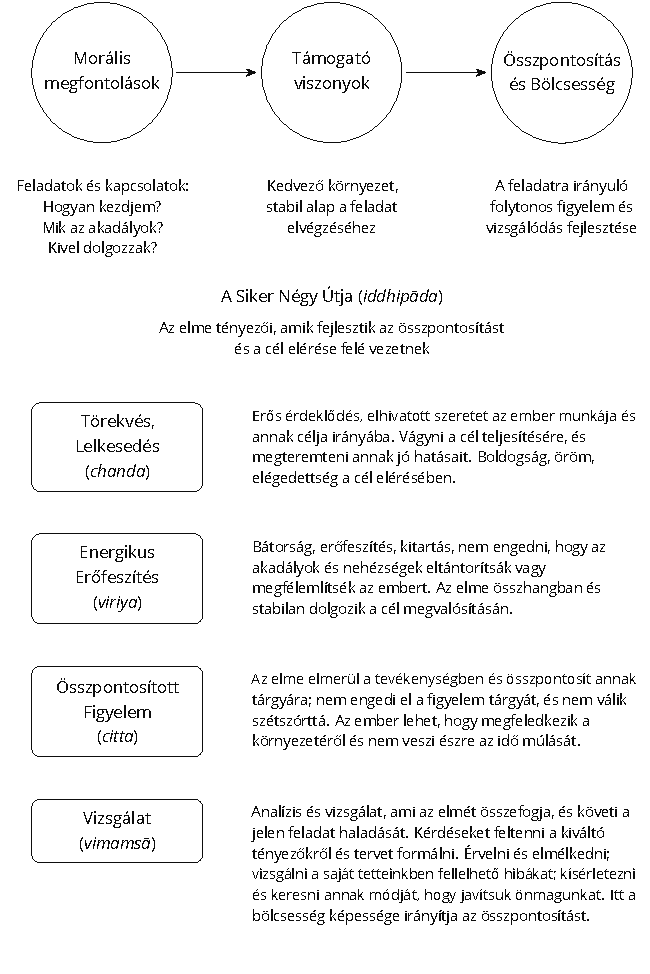
\includegraphics[width=0.95\linewidth]{./manuscript/tex/diagrams/paths-to-success-hu.pdf}
\end{figure}

\clearpage
\normalpagelayout

A csendes és nyugodt időszakok áldásnak számítanak. Mindig is értékeltem
egy stabil rutint, ami hosszú időszakokat enged a koncentrált munkára
vagy intenzív gyakorlásra. Más részről, akadályok és konfliktusok is
garantáltan jönni fognak.

Nem kell amiatt aggódnunk, hogy a meditáció meg fogja oldani minden
problémánkat, és nem lesz mit tennünk. A meditáció nem
probléma-megoldás. Ez az éberség olyan gyakorlása, ami túljut a belső
akadályokon és szembe néz a külső problémákkal, ahogy azok elénk
kerülnek. Ha egy fontos ügyet kell elintéznünk, segít, ha előbb
kitisztítjuk a fejünket. Viszont pusztán az, hogy ülünk a párnán mintha
túlhaladtunk volna minden problémán, a jelenre való tudatlanságot
gyakoroljuk, nem a tudatosságot.

Szándékosan szembe nézni és jó képességgel megbirkózni ezekkel arany
esélyt ad arra, hogy az elme képzését a korábbi korlátokon túl
fejlesszük. A zavaros káosz gazdag a lehetőségekben, hogy gyakorlati
úton fejlődjünk és tanuljunk.

Nem magukat az érzéseket keressük, nem különleges érzéseket próbálunk
létrehozni a meditációval, nem azt a helyzetet keressük, ahol mindig
minden jól megy nekünk. A kellemes, kellemetlen, semleges érzések
önmagukban nem adnak nekünk helyes megértést, ha követjük a befolyásukat
és gépiesen reagálunk rájuk. Az éberségnek észre kell vennie az
állandótlanságukat és bizonytalanságukat. Akkor megértéssel látjuk mi a
jótékony, és mi a kártékony a jelen helyzetben.

\keywords{csónak a folyón, én és enyém}

Könnyű a meditációt gyakorolni, vagy nehéz? Egy hasznos kép amire
gondolhatunk, ahogy egy csónak halad a folyón. Amikor a csónak áruval
töltött ládákkal van megrakva, a sok teher alatt nehezen és lassan
halad. Épp, hogy a víz felett tudja tartani magát.

Azt szeretnénk, hogy a csónakunk gyorsan haladjon, nem igaz? De
ugyanakkor ragaszkodunk mindenhez amivel megraktuk. Könnyítenünk kell a
csónakon, elengedni az `én' nehéz súlyát. Mi hozzuk létre az `én' és
`enyém' terhét. Mi hozzuk létre a benyomást, hogy `ilyen voltam, ilyen
vagyok, ilyen kell legyek'. `Az az enyém volt, ez az enyém, ez meg
akarom tartani, azt meg kell szereznem'. Ez a súly húzza le a csónakot.

Az érzés, hogy elég, ami van, megteremti a teret a nagylelkűségre. Az
elégedettség a gyakorlás folyamatos része, nem egy rögzült, feltételhez
kötött állapot. A tettek és a tanulás mint egy patak folynak az
elégedettségből. Mikor azt gondolom, `kész leszek elkezdeni, mikor már
megvan a \ldots{}', az elégedetlenség köti le a gondolataimat és folyton
megszakítja a koncentrációmat a jelen helyzetre.

\keywords{jótékony gondolatok, béke}

Viszont amikor azt gondolom, `nem vagyok jó ebben, de ennyi is elég,
hogy elkezdjem', elfogadni a jelen határaimat energiát ad a cselekvésre.
Végül gyakran többet is tudok tenni mint képzeltem.

A gondolkodás rossz hírnevet kap a meditációs könyvekben, de a tiszta
gondolatok megalapozzák a feltételeket a helyes hozzáállás fejlődéséhez.
Az elharapózó, kényszeres gondolkodás valóban fájdalmas tapasztalat, de
ha meg akarunk állítani minden gondolatot, mellé lövünk a célnak.

Vedd észre, hogy a jótékony gondolatokat megelégedettség és béke követi.
Erkölcsös tetteinket tudatosan felidézve kialakul a stabilitás és
ön-tisztelet érzete. Bízunk magunkban, hogy elengedjük ami fölösleges,
mert érezzük, hogy ami van az már elég.

Ha fejben akarjuk megoldani, a gyakorlás gyorsan bonyolulttá válik. A
meditációban, a testen keresztüli éberség egy megbízható irány: Az
érzéseket és elme állapotokat figyeljük, ahogy jönnek és mennek,
nézőpontunkat áthelyezzük, és nem magunkkal vagyunk elfoglalva. A
bonyolult kérdéseket magunk mögött tudjuk hagyni, mert már nincs
szükségünk a válaszokra.

\keywords{könnyű csónak, élvezetes tanulás}

Mi teszi lehetővé, hogy tovább tanuljunk és fejlődjünk? Az utazás akkor
a legélvezetesebb, amikor a horizont egyre tovább tágul, a korábbi
korlátainkon túl. A horizontot nem azzal tágítjuk, hogy messzire
utazunk, hanem azzal, hogy új szemmel látunk. A vágy, hogy megtartsuk
azt, amiről azt gondoljuk mi vagyunk, határozza meg a jelen korlátunkat.

A csónak könnyű, amikor üres az éntől és enyémtől. Nagy távolságokat
tesz meg dráma és zaj nélkül. Mi történik, ha a csónakban ülünk, és
valaki a csónakjával nekünk ütközik? Rákiáltunk, ellökjük az evezővel,
és egész nap erről panaszkodunk. Ez mind lehet, hogy jogos, de tönkre
tettük a napunkat a saját rossz társaságunkkal. Nehéz ebben a
bölcsességet látni. Mi történik, ha egy üres csónak ütközik nekünk?
Honnan eredt a korábbi harag és negatív indulat?

Hajlamosak vagyunk az én és enyémről szóló történeteket gyártani, akár
valós, akár képzeletbeli események alapján. Ha komolyan vesszük ezeket,
és valóságot adunk nekik, a történetek kezdenek irányítani minket, és
korábban nem létező problémákat hozunk létre.

\enlargethispage*{\baselineskip}

Előfordul, hogy ülünk a meditációs párnán, és vitákat kezdünk eljátszani
a képzelet bábjaival. Komoly az ügy, nekünk kell nyerni! Módszeresen
végig gondolni egy problémát hasznos eszköz, de önmagunk felé irányuló
szimpátiára és kedvességre is szükség van az építő jellegű belső
bárbeszédhez. Másként, amikor az én magával beszél, rossz társaságban
találja magát.

\keywords{aki tud önmagán nevetni}

Meglepő, mennyire fel tudjuk húzni magunkat egy olyan helyzettel
kapcsolatban, ami még meg sem történt. Segít, ha tartunk egy csipet
humort az oldal zsebünkben, vészes komolyság esetére. A görög filozófus,
Epiktétosz mondását felidézve, `Aki tud önmagán nevetni, sosem fogy ki a
nevetni valóból.'

\keywords{az érzékek egyszerűsége, elengedés}

A meditáció gyakorlásában visszaálltjuk a helyes szemléletet azzal, hogy
visszatérünk az érzékek egyszerűségéhez. A történeteket, ha vannak, a
változó körülmények nézőpontjából szemléljük. Az érzékek vizsgálatával
egy alapvetőbb valóságra alapozzuk a figyelmünket. A kellemes érzet
ilyen, ahogy most tapasztaljuk, a kellemetlen érzet ilyen, a semleges
érzet ilyen, kezdete van és vége, változik és üres.

A gyakorlásban nem az lesz értékes, hogy sietve eredményeket halmozunk
fel, hanem, hogy teret hagyunk az elengedésnek és türelemnek. Van amikor
cselekedni kell, de meglepően sokféle nehézséget megold az egyszerű
türelem. A sértettség vagy sürgető fontosság érzése magunkból ered. A
visszafogottság biztonságos nézőpontot nyújt ilyenkor, magunkkal és
másokkal szemben is. Engedjük a csónakunkat csendben tovább úszni.

\chapter{Csontok}

\keywords{testi fájdalom meditáció közben}

\noindent Még ha jó testtartással is ülünk, előbb vagy utóbb valami
valahol fájni fog. A jó testtartás minimalizálja a szükségtelen
kényelmetlenséget, de nem tudja teljesen megszüntetni. A fájdalom és
kényelmetlenség ténye együtt jár azzal, hogy van testünk, de nem azért
meditálunk, hogy kínozzuk magunkat, és ügyelhetünk arra, hogy elkerüljük
a sérülést.

A testi fájdalmat vizsgálhatjuk azt mint a meditáció tárgyát,
figyelhetünk a test egy másik területére, ahol nincs fájdalom, vagy
változtathatunk a testtartásunkon.

Ha a megszokott reakciónk a fájdalomra szorongás, ellenszenv és
nyugtalanság, akkor a vizsgálódás hasznosnak bizonyulhat. Emlékezz, hogy
a szándékod az, hogy jót akarsz magadnak. Ezután vizsgáld, figyeld meg a
fájdalmat, hogyan mozog a testben, hogyan keletkezik és múlik el
hullámokban. `Ki az, aki szenved? Változik ez? Hol van a tudatosság, ami
ezt tudja?' Ez megváltoztatja miként észleljük a fájdalmat. A
tapasztalatunk megváltozik, egy vészhelyzetből amit azonnal meg kell
oldanunk, egy jelzéssé, amit választásunk szerint félre tehetünk egy
időre.

Lehet, hogy a fájdalom nem jelent sérülést, mint például az ahhoz
hasonlítható kényelmetlenség, amit akkor érzünk, mikor végig kell ülnünk
egy hosszú utat a buszon. Választhatunk, hogy a figyelmünket a test egy
másik részén tartsuk. Vagy, a figyelmet módszeresen végig vezethetjük a
test különböző részein, megfigyelve a helyet, ahol nincs fájdalom, és
meditációnkat így folytatjuk, annak a területnek az érzeteit szemlélve.

Egy érdekes gyakorlat pontosan meghatározni, hol húzódnak a fájdalmas
terület határai. Éles ez a határ, vagy határozatlan? Rögzítve marad,
vagy fokozatosan más irányba tolódik? Az ilyen vizsgálat közben
megismerjük a fájdalom keletkező és elmúló természetét. Ezután már nem
olyan nagy ügy. Nem kell ellenszenvvel reagálnunk rá, tudunk hagyni némi
szabad teret a kellemetlen érzeteknek, hogy hadd legyenek.

Amikor eldöntöd, hogy ideje megmozdulni, mielőtt mozdulnál, állj meg egy
pillanatra és határozd meg tisztán a szándékot: `A testem iránti
együttérzésből mozdulok. Megváltoztatom a testtartásom, mert azt
kívánom, hogy a testem jól érezze magát és egészséges legyen.' Ezután
helyezd át a lábaidat, vagy válts testtartást. Ez egyben tartja az
éberség folytonosságát, és így nem az ellenszenvre vagy nyugtalanságra
reagálunk.

\keywords{a test vizsgálata, csontok, az 'én' képe}

Az ülő meditáció után, átválthatunk álló helyzetbe és hagyjuk az
ízületeket és izmokat ellazulni. Az álló helyzet több figyelmet igényel
az egyensúly megtartására, így a csontok, a test tartóelemei, jobban
érezhetőek.

A csontok a test központi, merev részeit képezik, amik meghatározzák az
alakját, mit képes és képtelen tenni. Csontok nélkül, a testünk egy
formátlan húspaca lenne. Csontokkal belső struktúrát nyer, ami megadja a
külső megjelenését, amit jól ismerünk. A tükörbe nézünk és azt
gondoljuk, `az én vagyok'.

\clearpage
\thispagestyle{empty}\mbox{}
\photoFullBleedPlaceholder{%
  TODO: Illustration of standing meditation.%
  \illustration{Álló Meditáció Testtartás}%
  \label{illus-standing-meditation}%
}
\clearpage

Mennyire vizsgáltuk meg a képet, mielőtt magunkat láttuk benne? Egy
rövid körvonal, kontraszt és szín máris kiváltja az `én' kép
megjelenését. Viszonylag állandó képünk van magunkról, a jelenben a több
évvel ezelőtti önmagunk képével azonosulunk. Mivel a változás lassú,
egyre kevesebb és kevesebb kulcs jellemzőre hagyatkozunk, hogy
felismerjük a tükörben látható képet.

Ha közelebb hajolunk és több jellemzőt látunk, vagy magunkat egy
szokatlan szögből mutatja egy fotó, percekbe is beletelhet mire el
tudjuk dönteni, kit látunk. Mi határozza meg ez a képet? Ha a csontok
egy kissé mások lennének, a testnek más alakja lenne, és ez
megváltoztatná nem csak a külsőnket, de azt is, hogyan élünk.

\keywords{álló meditáció módszere, álló testtartás}

Állj egyenes, de rugalmas helyzetben, fordíts egy kis idő arra, hogy
megtaláld a kiegyensúlyozott tartást. Helyezd a lábfejeket
vállszélességbe, a térdeket engedd ellazulni és kissé behajlani, hogy
aktív részük legyen a test megtartásában. Ne zárd az ízületeket
egyenesre, az megfeszíti őket és a tartásod merevvé válik. Tartsd a
lábfejeket párhuzamosan, a lábujjakkal egyenesen előre mutatva. Forgasd
a csípőt előre a vízszintes vonal mentén, kissé behúzva az alsó részt. A
mozdulat ahhoz hasonlít, mintha egy vödröt fordítanál a felső nyílással
magad felé.

Döntsd a tested jobbra-balra kissé, és érezd ki a súlypontot. Fejleszd
azt az érzést, hogy te tartod a tested egyenesben, hogy ne dőljön el. A
test egyensúlyát jobb a sarkok felett tartani, mint előre dőlni és a
lábfejekre nehezkedni.

Tartsd a vállakat elég szélesen ahhoz, hogy megnyissák a mellkast a
könnyű légzéshez, de nem olyan szélesen, hogy feszültté váljanak. A
kézfejeket kényelmes például a combokon tartani, körülbelül a pont
fölött, ahol a zsebek vannak egy nadrágon.

Engedj magadnak rugalmasságot, végezz kis változtatásokat a tartáson,
ahogy az izmok hozzászoknak a helyzethez. Érezd ki az állásban az
egyensúlyt és figyeld a testet ahogy így tartod. A gravitáció lefelé
húzza, nyomást hoz létre a földön. Ha úgy jobb, behajthatod a kezeket a
has előtt, egyik tenyér a másikon, kényelmes helyzetben.

A szemek lehetnek nyitva vagy csukva. Ha álmos vagy jobb, ha nyitott
szemmel meditálsz, de tartsd a tekinteted a magad előtti pár méteren. Ha
egyenesen előre nézel, a figyelem iránya kifelé fordul, és az ablakokban
látható mozgás elvonja a figyelmed.

Ha becsukod a szemed, de erőltetettnek és fájdalmasnak érzed, figyeld
hova irányul a szem fókusza, amikor becsukod. Ha befelé húzódik, mintha
egy közeli tárgyra fókuszálna a szemhéjak mögött, a szemgolyó belső
oldalán lévő izmok erőlködnek, hogy befelé húzzák azokat, ez a
feszültség szárazságot és könnycsordulást is okozhat.

A hagyományos Buddha szobrokon a Buddha szeme kissé nyitva van. Ő éber,
nem alszik. Ne zárd a szemhéjakat szorosra, gyakorold ellazítani azokat;
engedd le őket nyomás nélkül. Bár a szemhéjak majdnem zárva vannak,
képzeld azt, hogy egy távoli dologra nézel, ez hagyja ellazulni az
izmokat. Egy keskeny sáv nyitva marad, némi fényt enged be. Az is segít,
ha megmasszírozod a belső oldali szemizmokat, a nagyujjak hegyével
körkörös mozgásban.

Vegyél egy lélegzetet, és figyeld, hogyan változik a testtartás légzés
közben. A rekeszizom behúzza a levegőt, a has előre mozdul, hogy helyet
adjon. A kulcscsontok megemelkednek, a mellkasi bordák kifelé nyílnak, a
test súlypontja kissé elmozdul.

Van valami, ami korlátozza a légzést? Ellenőrizd, hogy egyenesen állj, a
váll ne görnyedjen előre, ami gátolja a nyitott légzést.

Figyelj a fej egyensúlyára, találd meg a pozíciót, ahol a fej a saját
súlyával egyensúlyban ül a gerinc tetején, nem dől előre vagy húzódik
hátra. Irányítsd a tekintetet kissé lefelé, ahelyett, hogy egyenesen
előre néznél, mert a jövés-menés elvonja a figyelmed. Húzd be az állat
könnyedén, ne engedd előre kitolódni, irányítsd a tekintetek pár
méterrel magad elé a földre. Engedd a fejtetőt kicsit megemelkedni,
mintha tartaná az eget.

A fej pozíciója nagy mértékben befolyásolja a felsőtest tartását. Mivel
sokat ülünk székeken, kialakul a szokásunk, hogy a fejet előre tolva
tartjuk, ez megfeszíti az hátizmokat a gerinc mentén. Ezeket az izmokat
nem tudjuk tudatosan irányítani, de kipróbálhatod, milyen érzés kissé
visszahúzni a fejet. Érzed ki az egyensúlyt, ahol a hátizmok ellazulnak.

Kiegyensúlyozott testtartásban a csontok úgy ülnek egymáson, mint az
óvatosan egymásra helyezett kövek. Ha a gerinc jó tartásban van, a
gravitáció elég, hogy stabilan tartsa. Ez kellemes, könnyed egyensúlyt
teremt erőltetés nélkül.

\enlargethispage*{\baselineskip}

\keywords{testhez való hozzáállás, analitikus elme, jószándék}

Ha túl analitikus hozzáállással közelítjük meg a test vizsgálatát, ez
groteszk és sokkoló benyomásokat kavarhat fel. A magunk felé irányuló
jószándék tartja a meditációt egyensúlyban, és hozzáállásunk jótékony
marad.

Az intellektus működése során elvont fogalmakat épít, figyelmének
tárgyait elkülöníti az egésztől. Mikor a testet szemléli, lehet, hogy
annak különböző részeit absztrakt és élettelen tárgyként tekinti.
Emlékezzünk, hogy nem azért gyakoroljuk a meditációt, hogy a testtel
szemben ellenszenvet vagy elidegenedést keltsünk. A meditáció tiszta
megértése akkor működik jól, amikor a dolgokat a környezetükkel együtt
látja, semmi nem létezik elszigetelve, üres térben. A tudatosság
befogad, nem kizár, és ehhez a hozzáállásunk része kell legyen a nyitott
elfogadás és jószándék.

Ez a hozzáállásbeli különbség egy történetre emlékeztet Platónról és
Diogenészről. Platón éppen egy előadást tartott a diákjainak Athénban az
Akadémián, és az `ember' fogalmát úgy határozta meg, mint `tollatlan
kétlábúak'. Úgy esett, hogy Diogenész hallotta ezt, és mivel kedvelte az
gyakorlatias vicceket, behozott az Akadémiára egy kopasztott csirkét, és
feltartotta Platónnak, ``Íme! Hoztam neked egy embert.'' Úgy
gondolhatta, ez bemutatja, hogy bizonyos környezeti jellemzők hiányoznak
az ember túlságosan intellektuális meghatározásából, mint `tollatlan
kétlábú'.

A csoport az Akadémián kiegészítette a meghatározást, ``\ldots{} lapos
és széles körmökkel'', ami kielégítette az intellektuális tárgyalásukat,
de alighanem nem értették meg mire mutatott rá Diogenész.

\keywords{az egész testet megtapasztalni}

Figyeljük a testi érzéseket a belégzés és kilégzés közben. Irányítsd a
figyelmet befelé, éberen a benyomásra, hogy `a test ilyen'. Az elme nem
keres, nem a világban jár valahol. Nem igényel semmit, ami itt van az
elég. Éberséggel látjuk a testet, a lábfejeket, a lábakat, a hasat, a
mellkast, a karokat, a vállakat, a nyakat és a fejet. Az test egy
egészet alkot, egy mozgó benyomás, érzékeny a lélegzetre.

A testet így figyelni olyan, mint az esőt nézni. Nincs tennivaló, semmit
nem kell eldönteni. Az eső tovább folytatja a dolgát anélkül, hogy be
kellene avatkoznunk.

\keywords{tiszta megértés, testre irányuló tudatosság, kioltani a haragot és vágyat}

A kártékony gondolatokat hasonlíthatjuk a szélben kavargó porhoz:
elhomályosítja a képet, nem látunk tőle semmit. A Buddha az éberség
hatását az elmére az esőhöz hasonlította, ahogy kimossa a port és
megtisztítja a levegőt. `Szüntesd meg az ilyen (kártékony) gondolatokat
és kérdéseket, ahogy az eső elmossa a port; A szívben elcsitulnak a
gondolatok, és helyben eléri a béke állapotát.'\footnote{\href{https://suttacentral.net/iti87/en/sujato}{Iti
  87}, A Látás Pusztítói}

Az elmére való éberség megállítja a kártékony jellemzők keletkezését,
fejleszti a jótékony jellemzőket, és így megtisztítja az elmét.
Észrevehetjük, hogy a világot nem egy rögzített módon tapasztaljuk: nem
elzárt, külső szemlélők vagyunk, mintha egy magunktól különálló világra
néznénk az ablakon át. Aktív szerepünk van a világ létrehozásában, amit
tapasztalunk, hiszen mi alkotjuk a benyomásait a figyelmünk módján
keresztül.

Amikor megalapoztad a tiszta megértést, és észreveszed, hogy az elme
egyre tisztább és stabilabb, vedd szemügyre, mi tette lehetővé ezt a
változást? Mit tettél? Mit \emph{nem} tettél? Nem kellett az érzéki
benyomásokat manipulálnod, vagy küzdened a gondolatokkal és érzelmekkel,
elegendő volt megváltoztatni a figyelem módját.

A figyelmünk módja hozza létre a referencia keretet, amiben
megtapasztaljuk az érzékek világát az észlelések és emlékek felfogásától
függően. Ez egy folyamat, ami egy bizonyos hozzáállást produkál, mint
egy, az időt feldolgozó függvényt, aminek eredményétől függően
felismerjük és értelmezzük önmagunkat a jelenben.

A figyelem változását arra használjuk, hogy ne tápláljuk tovább a
kártékony mentális tényezőket. A közvetlen tapasztalat szemszögéből,
annak megfelelően ahogy a dolgok vannak, végük szakad, a folytatáshoz
szükséges referencia pont nélkül.

Röviden úgy mondjuk, az elmére való éberség megtisztítja az elmét.

A testi tudatosság felé fordulunk, ami kioltja mind a haragot és vágyat.
Megváltoztatja a figyelmünk keretét, hasra esnek mintha kihúztuk volna
alóluk a szőnyeget. A zsúfolt, kritikus és haragos gondolatok olyanok,
mint egy zajos műsor, vagy a hírek a tavalyi újságban. A témája már nem
érdekel minket, elvesztette a fontosságát, folyton csak körbe-körbe jár.
Tedd le a gondolkodást, mint egy fáradt túrázó a nehéz hátizsákot, és
maradj a test éber figyelmével.

Időnként elvonja valami a figyelmünket, vagy elkezdünk álmodozni; mindig
térj vissza a légzéshez és az álló helyzet testi érzéseihez. Ha állás
közben csak történetekről és belső fantáziákról gondolkodunk amíg meg
nem szólal a harang, azzal nem a belátás meditációt gyakoroljuk\ldots{}
hanem a buszra várakozást.

\clearpage

\keywords{emlékek mint én, történetek az énről}

Vizsgáld az elme állapotát mint tapasztalatot. A test észlelése és az
érzései azelőtt jelennek meg, hogy az `én' észlelését felépítenénk
belőle. Mire emlékszünk önmagunkról? Ha elfelejtjük, amikor tegnap
valaki gorombán ránk kiabált, vagy emlékezünk, amikor barátainkkal
töltöttük az időt, ez megváltoztatja miként tekintünk önmagunkra?

Ez a kapcsolat az emlékeink, érzéseink és elme állapotunk között folyton
változik. A felfogott képek folyton változnak, az éber tudatosság
megismerésével a bizalmat abba helyezzük, ami ismeri ezt a változást.
Ezzel a változást egy nagyobb képen belül láthatjuk, és nem ragadunk meg
a félelemben. Önmagunk képét egy aktív folyamat hozza létre, részt
veszünk benne az emlékeinkkel, azok újra-értelmezésével. Felépítünk egy
történetet magunkról a múlt emlékeiből, és megválasztjuk mit teszünk
most.

\keywords{csontok, a test részei, megfelelni akarás, a külső megjelenés bírálata}

A testet és annak részeit szemlélve az elmét a változó benyomásokra
összpontosítjuk, mielőtt az `én' képe megjelenik. Ez a folyamat
lefegyverzi az ön-bírálatot, a félelmet és elvárásokat, amik mint a
mocsár lehúznak minket.

\enlargethispage*{\baselineskip}

Figyeld az érzést, ahogy a csontok kapcsolódnak egymáshoz az
ízületeknél. Megjelenik egy belső struktúra érzete, a struktúra ami a
testet belülről tartja. Merev darabok, egyik vég a másikhoz kapcsolódik,
egymásra rakva egyre magasabbra. A lábakban érezzük a merev csontokat,
ahogy tartják a testünket. Az érzés a gravitációról és nyomásról
árulkodik. A csípő csont a lábakon nyugszik, a felső test ehhez
kapcsolva mozog. A mellkas bordái szétnyílnak és összehúzódnak a
légzéssel. A gerinc ív alakban tartja a súlyt. A fej ott ül a gerinc
tetején. A koponya csontjai megfeszítik az arcbőrt.

A testünk darabokból áll. Darabokból, amik egyes helyeken merevek, más
helyeken puhák és rugalmasak. Ezek együttállása adja meg a formáját.
Amikor egy személyre nézünk, nem látunk mást, mint a hajat a fejen, a
szőrt a testen, körmöket, fogakat és bőrt. Ebből építjük a személyt --
elég a másodperc törtrészéig rápillantanunk, felismerni egy körvonalat
vagy jellemzőt, és azt gondoljuk, `Ez én vagyok. Jól nézek ki?'

Egyes helyzetekben láthatjuk a fokozatos felismerést az általánostól az
egyéniig, például amikor valakit látunk a ködben sétálni. Először
észrevesszük, hogy ez egy `személy' alakja, azután férfi vagy nő. Lehet,
hogy valaki akit ismerünk? Végül egy részlet kiváltja egy barátunk
felismerését és eszünkbe jut a neve. Mindez az észlelés képeinek
világában játszódik le.

Szokásunk, hogy a saját testünket, és másokét, egy töretlen egységként
látjuk, egyetlen dologként. Ebből a nézőpontból kialakul a megrögzött
gondolat, hogy van egy ideális formája és állapota. Elvárjuk, hogy a
testnek legyen bizonyos formája, magas vagy alacsony, és a további
jellemzői.

Ezek világi bírálatok, képek amit a kultúra amiben felnőttünk alakított
ki bennünk. Az egyik kultúra a vékony, a másik a telt testet tekinti
ideálisnak, és ezek a kulturális ideálok is változnak egyik generációról
a másikra. A hirdetések és a média üzenetei megerősítik ezeket az
elvárásokat és gondolat nélkül hiszünk bennük. Amikor közelebbről
szemügyre vesszük, azt látjuk, ezek egy ferde tükör képei, nem egyeznek
a valósággal.

\clearpage

\enlargethispage*{3\baselineskip}

\begin{figure}[h]
\caption{Experience and Illusion of Self}\label{fig-illusion-of-self}

\centering

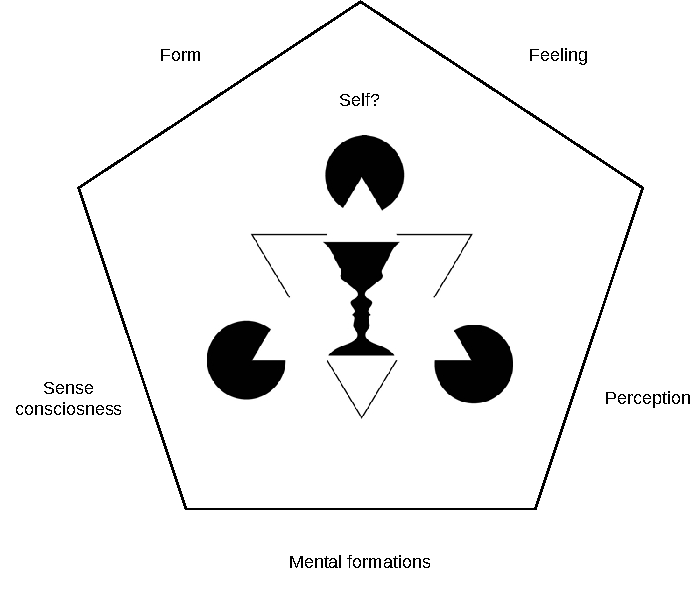
\includegraphics[width=80mm]{khandhas-self-illusion.pdf}

\bigskip

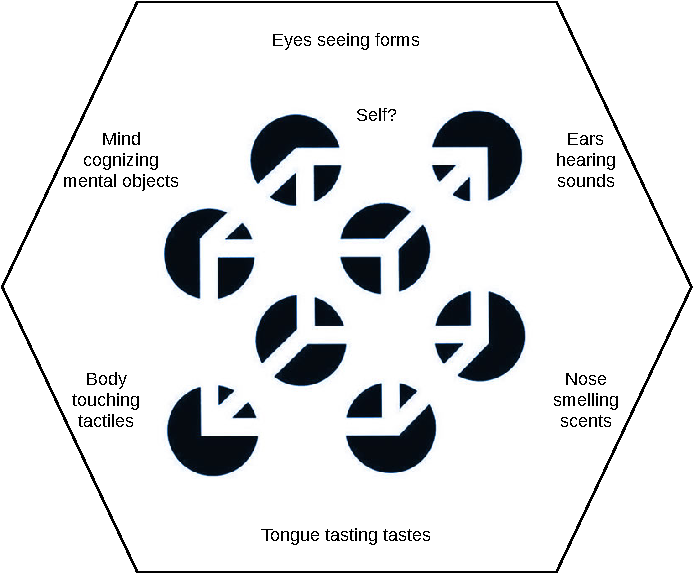
\includegraphics[width=80mm]{senses-self-illusion.pdf}

\bigskip

{\small
We experience a self, which has no substance beyond that experience.
Above, conditioned expectations create filled-in shapes which we \emph{experience}, but are not there.
The Kanizsa Triangle, Rubin's Vase and Subjective Necker Cube are examples of illusory contours.
}

% FIXME TODO translate figure text

\end{figure}

\clearpage

Lehet, hogy mi sokat gondolunk arra, hogy mások mit gondolnak rólunk, de
\emph{mi magunk} mennyit törődünk mások küllemével? Ha magamat figyelem,
nem foglalkozok sokat más emberek kinézetével. De én zavarban tudom
érezni magam, és azt képzelem \emph{ők} biztos \emph{rólam}
gondolkodnak. Mikor, valójában, annyit gondolnak rám mint én rájuk --
alig, ha egyáltalán. A saját életükkel vannak elfoglalva, mint ahogy én
is az enyémmel.

Az önbírálatunk nyomása mellett, elképzeljük mások hogyan bírálnak
minket. Mivel nem tudhatjuk és nem irányíthatjuk mit gondolnak, az elme
belső párbeszédével megpróbáljuk megteremteni ezt a tudást és
irányítást, ami illúzió marad. Amikor lejátsszuk ezeket a belső
párbeszédeket, élvezzük ezt a megfoghatatlan irányítást. Viszont
lemaradunk arról a szabadságról, ami az irányítás igényének
elengedéséből születik.

\keywords{a test részeinek éntelen jellege}

Megfigyelhetjük az aggodalom feltételektől függő természetét, amikor a
test egyes részei elválnak. Sokat foglalkoztathat minket a hajunk
például, de csak addig, amíg a fejünkön van. Amikor a fodrász levágja,
nem törődünk a padlón összegyűlt hajkupaccal. Hasonló módon, mikor a
körmünket vágjuk, mikor van az a pont, amikor már nem `én' és `enyém'?

Így vizsgáljuk a testet, mint ami darabokból áll össze, és látjuk, hogy
a test nem egy bontatlan egység. Darabokból és részekből áll, amiknek
megvan a maguk természete, és aszerint viselkednek, nem hallgatnak a mi
vagy mások véleményére. Csontok, bőr, haj, fogak és körmök: olyanok
amilyenek, a saját természetüknek megfelelően.

\clearpage

A testünk egy áldás. Nem azért gyakoroljuk a meditációt, hogy
ellenszenvet keltsünk felé. Az egészség egy áldás, támogat minket
mindenben, amit teszünk. A Buddha az egészséget a legnagyobb kincsnek
nevezte.

\keywords{történetek mint álmok, testre irányuló tudatosság, szürke és élettelen állapotok, hála érzet}

Figyeljük a légzést, a test részeit, a jelen tapasztalatunkat. Azt
találjuk, hogy nem hordozzák magukkal az `én' és `enyém' történeteit.
Mivel mi hozzuk létre ezeket a történeteket, meg is tudjuk állítani
őket, nem vagyunk hozzájuk láncolva. A jelenségek függő kapcsolatokon
keresztül létre jönnek, a kapcsolat felbomlásával megszűnnek. Ez minden
ami történik.

A testre irányuló tudatosság enged a kívánságok szorításán és rávezet
arra, hogy szerencsések vagyunk, hogy itt lehetünk. Ehhez a figyelemhez
mindig vissza tudunk térni, egy belégzés és kilégzés elég ahhoz, hogy
emlékezzünk a keletkezésre és elmúlására. A kétségek olyanná válnak,
mint a sztorik egy régi újságban. A múlt szálait nehéz követni és
fáradtságos kibogozni, mintha valaki más álmait kellene értelmeznünk.

Ami valós, az mindig itt van a jelen tapasztalatunkban. Nem az válik
fontossá, hogy mik vagy kik vagyunk a történetben, hanem az, hogy a
figyelmünket a jelennek tudjuk szentelni.

\enlargethispage*{\baselineskip}

A tiszta szándéknak fontos szerepe van. Amikor nincs tisztán
elhatározott szándékunk, egyszerűen csak sodródunk. Nem kifejezetten
zavar minket, hogy itt vagyunk, de az elme szürke és élettelen, egy
jövőbeli időre vár, és addig próbál elbújni és láthatatlanná válni. Az
eredmény, hogy valóban szürkévé és láthatatlanná válunk. Semmi rossz nem
történik, de nincs semmi fény és öröm abban, hogy itt vagyunk.

Nem állunk meg elég gyakran, hogy észrevegyük mikor boldogok és
nyugodtak vagyunk. Amikor az elme tiszta és csendes, természetes módon
hálás azért ami itt van, és az áldásokért amit életünkben kaptunk.

A hálát nem lehet akarattal erőltetni. A gyakorlásban nem létrehozunk
valamit, hanem tiszta szándékkal felismerjük azt ami itt van. Nem erő
vagy képesség kérdése, ezek időhöz és körülményhez kötöttek. Az
elhatározás, a befelé irányuló felismerő figyelem nem egy adott
körülményhez kötött. Az eredmény a helyes szemlélet, amiben látjuk a
dolgok megfelelő helyét, és mit kell azokkal tenni -- vagy csak
megállni, figyelni és lélegezni.

\chapter{Pocsékul}

\section{Egy Felépített Kép}

\begin{itemize}
\tightlist
\item
  Helló, hogy érzed magad?
\item
  Pocsékul.
\end{itemize}

Egy meditáló embernek nem ezt kellene mondania, ugye? Pozitívan kellene
válaszoljon, mint például, `Remekül érzem magam, csodás napunk van!',
vagy legalább, `Én megvagyok, és te hogy vagy?' Van a fejünkben egy kép
a `meditálóról', akitől elvárjuk, hogy bizonyos módon viselkedjen és
beszéljen, és bizonyos más dolgok nem illenek hozzá. Hogy került a
fejünkbe ez a kép?

A `jó meditáló' képe egy felületes benyomások alapján kialakult
észlelés, amiről engedtük magunkat, hogy valósnak tekintsük mélyebb
vizsgálat nélkül. Gondolj arra, mikor megnyitottál egy meditációról
szóló cikket. (Miközben tovább olvasod a jelenlegit\ldots) Egy
fényképpel kezdődik amin egy szerzetes vagy meditációs világi tanító
mosolyog, és az éberség pozitív hatásairól szóló leírással folytatódik.
Esetleg egy elvonuláson készült fényképeket és történeteket is
tartalmaz. Az emberek békés arccal ülnek a meditációs párnákon, míg az
ablakon keresztül áradó fény megvilágítja a Buddha szobrot. Lentebb egy
interjú részlet olvasható benne arról, hogy valaki hogyan jutott túl a
belső küzdelmein. Egy meditációs tanító bátorító szavaival zárul a
tiszta elme erejéről, vagy egy idézettel a Buddhától.

Még akit nem is érdekel túlságosan a meditáció is tudja milyen egy ilyen
cikk, mind láttunk már több tucatot. Nincs szükség itt forrás szöveget
megjelölnöm, ebben a könyvben található fejezetek is például
szolgálhatnak.

Ezzel nem arra akarok utalni, hogy félre akarnának vezetni. A szerzők jó
szándékkal teszik ezt, hogy bátorítsanak minket a vizsgálódás ösvényén
haladni és hogy tegyünk erőfeszítést a gyakorlásunkban. Ha a
frusztrációkon túl nem látható semmilyen nagyobb boldogság, mi az
értelme az egésznek? Ha csak kín és szenvedés lenne várható, azt
segítség nélkül is létre tudjuk hozni magunknak.

A buddhizmus alapvetően optimista, és központi témája a boldogság. Saját
hozzáállásunk, hogy a boldogságot keressük, vagy létre akarjuk hozni.
Míg ezzel foglaljuk el magunkat, csak egyre keserűbbek leszünk, és úgy
tűnik ez sosem lesz megvalósítható. Emiatt a körülményeket, vagy saját
képességünket tartjuk elégtelennek, de valójában a dolgok természetes
működését nem értjük, és hozzáállásunk ezért vezet helytelen irányba. A
feladatunk, nem az, hogy a boldogságot keressük, hanem, hogy a szenvedés
keletkezését megértsük, és ne hozzuk azt létre. Ennek megértésén
keresztül az elmében spontán megjelenik a boldogság.

A tanítások valóban sokat említik a szenvedést, de az utasítások arra
alapulnak, hogy a szabadulás ettől a szenvedéstől lehetséges. A Buddha
világosan kifejtette, hogy az út gyümölcse őszinte boldogság, és ha ezt
gyakorolni nem lenne lehetséges, vagyis elhagyni a kártékony gyökereket
és fejleszteni a jótékonyakat, nem tanítaná azt.\footnote{\href{https://suttacentral.net/an2.11-20/en/thanissaro}{AN
  2.19}}

Ki ez a meditáló a fejünkben? Egy dolog biztos, aki az \emph{én
fejemben} van, mindig \emph{jobban tud meditálni} mint én. Amikor valaki
egy jó fotót készít rólunk, tudjuk hogy van ez: egy rendezett, jó
pillanat volt, de tudjuk, hogy öt percen belül akár az ellenkezője is
igaz lehet. Habár ez másokra is érvényes, nem csak magunkra, valahogy
nem emlékszünk erre amikor másokról készül jó fotókat látunk.

\section{Szálak}

A Buddha idejében az irodalom egyik formája a \emph{szutta} volt, ami
egy párbeszéd szálat jelent. Ez tartalmazhat prózai és verses szöveget
is, azzal a szándékkal, hogy szavaláson keresztül lehessen őket
memorizálni. Egy spontán mindennapos eseményt, vagy szervezett közösségi
gyűlést követően ami tisztán érthető példája volt a tanításoknak, a
közösség formális alakba öntötte a történetet és szuttaként szóban
memorizálták azt. Erre a Buddha is szorgalmazta őket:

\begin{quote}
Így kell gyakorolnotok: `Jól oda fogunk figyelni, amikor a
tanítóbeszédeket recitálják, amelyek a Tathágata mélységes, mély
jelentésű, páratlan, az ürességre vonatkozó szavai. Hegyezni fogjuk a
fülünket, kitárjuk a szívünket a megismerésük felé. Úgy tekintünk rájuk,
mint amit megéri megragadni és a mesterévé válni.'
(\href{https://a-buddha-ujja.hu/sn-20.7/hu/fenyvesi-robert}{SN 20.7})
\end{quote}

Manapság a könyvek, cikkek, blog posztok töltik be ezt a szerepet,
melyek a kánon szuttáit tartják maguk előtt példaként. A korai idők
szerzetesei ezeken a szálakon keresztül juttatták el hozzánk üzenetüket,
ez részévé válik az egymás közötti párbeszédünknek azokkal, akikkel ma
találkozunk, és írott munkáink azokhoz szólnak a jövőben, akikkel mi már
nem találkozunk.

Viszont a mai szociális médiában az üzenet világos megértését torzítja
az úgynevezett `Instagram effektus', ami egy szelekciós elfogultság
afelé, hogy a legjobb és legpozitívabb oldalunkat mutassuk, és szűrjük
ki a negatívat, ami ennek ellenére éppen olyan valóságos és szükséges az
egész kép teljes megértéséhez.

Gondold végig az írás folyamatát. A szerzőnek van egy mondandója, ami
egy cél lesz amihez igazodjunk, vagy egy tapasztalat amit felismerjünk.
Kiválaszt egy sor személyes tapasztalatot, véleményt, és megerősítő
magyarázatot más szerzőktől.

A szerző írhat igazság-hűen és próbálhatja elkerülni az `Instagram
effektus' szelekciós elfogultságát, de valamilyen szűrő mindig
működésben van. A saját tapasztalatából választ és bemutat egy szeletet,
lefordítva azt az olvasók kultúrájának kifejezéseire, olyan példákra
építve, amik (remélhetőleg) ismerősek azon olvasóknak. Az írott szó
világa mindig egy felépített valóság. Viszont, ha jól el van találva,
ráismerünk benne a saját tapasztalatunkra.

A meditáló, aki a fejünkben él olyan, mint egy versben szereplő
karakter, vagy egy mítoszban szereplő hős. Bölcsebbek és erősebbek
lehetnek nálunk, hogy amikor elveszettnek és gyengének érezzük magunkat,
hitet és tanácsot tudnak nekünk adni. Az ő békéjük megrendíthetetlen
lehet, hogy amikor pocsékul érezzük magunkat, képesek legyünk kiállni
azt és várni amíg a nehézség véget nem ér.

Az ilyen felépített mentális képeket nem tekinthetjük valódi személynek.
Értékes források amikkel önmagunknak irányt mutathatunk, a történet
leírása segít kitalálnunk mit tegyünk azzal, hogy megmutatja hol vagyunk
egy nagyobb kép keretén belül. Egy mentális kép szerepe nem az, hogy
\emph{mivé kellene váljunk}. Amikor ezt próbáljuk elérni,
önellentmondásokba keveredünk és elégtelennek érezzük magunkat, mert az
élet valós körülményei sokkal összetettebbek, képlékeny és változó
határokkal, nem mint egy kép leegyszerűsített valósága. A kép egy eszköz
a magyarázatra, egy adott világra tekintő \emph{látásmód}, és egy példa
a helyes cselekvés módjára abban a fajta világban.

\section{Feltevések}

Felidézhetjük a Dhammapada verset, ami rámutat, hogy a tapasztalatunk
világa nem független tőlünk:

\begin{quote}
Az elme minden létállapot előtt jár, az elme vezeti őket, az elméből
származnak. (Dhp 1)
\end{quote}

Hogyan tesztelhetjük, hogy képzeletbeli problémákat gyártunk magunknak,
vagy a tettre késztető nyomás egy fontos jel, amit nem kellene figyelmen
kívül hagynunk?

Először megkérdezhetjük, `Képes az alany szenvedést tapasztalni?'
Élőlények szenvedhetnek, de egy kulturális fogalom, vagy magunk által
létrehozott történet nem tud szenvedni, még ha közben \emph{mi}
szenvedünk is. Megváltoztatja a hozzáállásunkat, ha az aggodalmunk
tárgya csak történetként létezik, mint egy intézmény, nemzet, pénz,
hírnév vagy egyéb társadalmi történet, és nem egy élő lény.

Ezt követheti egy gyors morális biztonsági teszt: `Egy bölcs ember vajon
dicsérné vagy kritizálná ezt?'

Majd visszaemlékezve kibogozhatjuk a nézetet: `Milyen feltevés hozza
létre ezt a feszültséget és nyomást? Mi ad jelentést nekem ahhoz, hogy
ezt tegyem? Mi az, ami nélkül ennek nem lenne jelentősége?'

Feltárhatjuk az ilyen tudattalan motivációkat azzal, hogy a jelen
tetteinket és választásainkat figyeljük. Ami már kifejezésre került,
implicit tartalmazza az információt, ami a megjelenéséhez szükséges
volt. `Miért választom megtenni ezt, itt? Honnan ered ez a tett és hova
vezet?' A mögöttes tényezők eredhetnek például a környezetünk által
kondicionált szokásokból, és eddig sosem fejeztük ki gondolatban miért
tesszük amit teszünk, csak a tett eredményét éreztük magunkon, legyen az
jó vagy rossz.

A tettekkel kezdeni a vizsgálatot és úgy rákérdezni a gondolatokra egy
megbízhatóbb módszernek bizonyulhat, mert a belső csevegésünk közben
mindenféle belső ellentmondásokat mondunk magunknak, viszont egy tett
már ad egy világos referencia pontot.

A hozzá kapcsolódó érzés lehet, hogy pocsék, de ha ezt jelzésként
kezeljük arra, hogy forduljunk az elme felé és vizsgáljuk azt, a
hozzáállásunk gyakorlatias és eredményes maradhat. `Ha már egyszer itt
vagyok, mit tanulhatok ebből?'

A feltevéseinkhez azon keresztül találunk hozzáférést, hogy felfedjük a
tudattalan motivációinkat -- ha egyszer már tisztán ki tudunk fejezni
egy feltevést, szabadságot nyerünk arra, hogy megfordítsuk, vagy
elhagyjuk azt. Megkérdezhetjük, `Segít ebben a helyzetben, ha
megfordítom a feltevéseimet?' Talán az, hogy az ellenkező irányból
tekintünk rá lesz éppen az, amire szükségünk volt a megbékélésre, a
tisztánlátásra a folytatáshoz, vagy ahhoz, hogy elhagyjuk az egész ügyet
mint ami sosem létezett. Akárhogy is, már nem kényszerből cselekszünk:
szabadok vagyunk elengedni vagy \emph{választani} azt, hogy végig
folytatjuk.

\section{A Vihar Után}

Amikor az utasítás azt mondja, `tér vissza a jelen pillanathoz', ez nem
jelenti, hogy mindent szeretned kell amit ott találsz, de ez az egyetlen
hely ahol élni tudsz. Ha boldog vagy, nem a jövőben vagy boldog, hanem a
jelenben. Ha szenvedsz, nem értheted meg a jövőben, csak a jelenben.
Egyes helyzeteket semmilyen agyalás és belső párbeszéd nem fog javítani,
legjobb úgy nevezni ahogy az van, és méltósággal eltűrni. Egy konfliktus
őszintén feszültséggel teli, elválni attól amit szeretünk mindig szomorú
lesz, és életben lenni mindig a saját halálunk tragédiájával végződik.

Hajlamosak vagyunk a sikert várni, és számítunk arra, hogy a kemény
munkánk a jövőben igazolódik. Vedd szemügyre óvatosan a siker
pillanatát, mit tapasztalsz? Lehet meglepetés, öröm, vidámság,
megkönnyebbülés, az után minden visszatér a hétköznapi szintre. A célról
kiderül, hogy nem az, aminek gondoltunk, és ha intenzíven arra
koncentráltunk, hogy oda jussunk, talán nem is emlékszünk semmire az
odavezető útról, és bánkódunk, hogy elmulasztottuk. Olyan erősen leköt
minket az, hogy eredményesek legyünk, hogy elpazaroljuk a lehetőségünket
arra, hogy éljünk.

A halál felett szemlélődni egy igazmondó, noha kissé ilyesztő, tükröt
tart az értékeink elé. `Ha ma este meghalok, boldogan emlékeznék arra,
hogy úgy élek, ahogy ma teszem?' Ez a kérdés többet fel tud kavarni a
mélyből, mint amire vállalkoztunk. Emlékszem olyan időre, amikor a
válaszom a `boldog' szóra kizárólag harag és önutálat volt.

A `hedonikus taposómalom' kifejezés leírja az adaptív folyamatot, amiben
a sikeres eredmények érzelmi hatása a normális szintre csökken az
elmében, és visszaáll a szokásos érzelmi állapotunk. Mintha
taposómalomban járnánk, nem számít milyen erősen próbálja az ember
növelni a boldogság szintét sikerek elérésével, az ember csak egy
helyben marad. Az életünket azzal töltjük, hogy az úton utazunk, nem a
célállomásban. Ha közelebbről megnézzük, még a célállomás puszta ötlete
is szétfoszlik, minta mikor berepülünk egy felhőbe. `Azt hittem ott
látom, de most, hogy ott vagyok, itt semmi sincs.'

Az bölcsek figyelmeztetnek erre minket, de úgy látszik szenvednünk kell
mielőtt figyelni kezdünk, hogy megértsük mi az a probléma amiről
beszélnek. Szókratész azt mondja, `Óvakodj a nyüzsgő élet
terméketlenségétől', de abból amit az életéről tudunk, nekem úgy tűnik
egy aktív és törekvő ember volt. Talán ez nem ellentmondás, ha az ember
örömét a jelenben találja, és nem a jövőre néző elvárásokban keresi. Azt
is mondja, `A boldogság titka nem a több keresésében rejlik, hanem
abban, hogy képesek vagyunk élvezni a kevesebbet.'

Könnyen túl-korrigáljuk a nyüzsgést, és átesünk a másik végletbe, azt
gondolva, `Elegem van! Megszabadulok mindentől!' Az önutálat
``logikusnak'' tűnhet, még ha tovább folytatja is a szenvedést. Sokan
vagyunk, akik könnyen kritizáljuk magunkat, és szorgalmasan gyakoroljuk
ezt, olyan meggyőződéssel igyekszünk bebizonyítani a saját tévedésünket,
mintha az ön-ellenszenv egy erény lenne. `Pocsékul érzem magam, aki
\emph{valóban} meditál sosem érezné így magát. Biztos, hogy valamit
rosszul csinálok.' Egy egész ön-azonosságot fel lehet építeni ekörül,
ami mindig panaszokkal és ön-ellenszenvvel válaszol. Egy adott személy
évtizedeken át élhet így, és ez válik az alap szintté, ami alapján
felismerik magukat. `Ha nem lennék ilyen mérges, nem is tudnám ki
vagyok.'

Olyan ez, mint beragadni egy tükrökből készült labirintusba: bárhova
nézel, csak magadat látod. A menekülés kulcsa, hogy találjunk egy
repedést a tükrökön és ismerjük fel a változást: az hajtott érzés,
szorongás, harag, motivációk amikről azt gondoltuk állandóak, valójában
folyton változnak, szétesnek és újra formálódnak. A labirintust az elme
hozta létre, és amit létrehozott üres az éntől, nem lehet az, ami
valójában mi vagyunk.

Tudunk benne meggyőző logikát találni, és az érvelésünk a kritikus
hozzáállásunk védelmében teljesen észszerű lehet! A pszichológusok azt
mondják, hogy a legnehezebben kezelhető betegeik azok, akik
intelligensen védik és indokolják saját rossz szokásaikat. Emlékszel
magadra, amikor te játszottad a keserű filozófus szerepét? Olyan okosak
tudunk lenni, semmi esély arra, hogy boldogok legyünk, és be is tudjuk
bizonyítani.

Nem szükségszerűen jelent azonnali megkönnyebbülést, amikor
ön-vizsgálatunk felfedi nekünk az eddig keresett értékeink ürességét. A
harag, kétségbeesés\footnote{A Buddha a haraggal és kétségbeeséssel való
  küszködést ahhoz hasonlítja, mintha egy ösvényt követnénk, ami mellett
  mély szakadék tátong.
  (\href{https://www.accesstoinsight.org/tipitaka/sn/sn22/sn22.084.than.html}{SN
  22.84})

  A türelmes kitartás egy alábecsült erény, de gyakran nincs másra
  szükségünk, csak hogy eszünkbe jusson várni: a kavargó elme állapotok
  drámai eső és villámlása ki fogja magát futni. Amikor megjelenik a
  hála érzete, az olyan jel, mint a vihar utáni szivárvány. Jótékony
  elme állapotokat kísér, és intelligensen több szögből is látjuk a
  helyzetet: egy jó alap arra, hogy segítőkész gondolatok jelenjenek meg
  arról, mit tegyünk. Néha az a legjobb, ha egyszerűsítünk és
  elfordulunk régi szokások és értékektől, Máskor, már megváltozott a
  nézetünk, és talán tovább folytatjuk amivel eddig foglalkoztunk, de
  hátra hagyva a nagy sietséget, azért folytatjuk, hogy azt éljük, nem
  mert a jövőt várjuk.

  \begin{quote}
  A múltat ne kergesd,\\
  és ne álmodozz a jövőről.\\
  Ami elmúlt az már mögöttünk van.\\
  Ami eljön azt még nem értük el.

  \emph{MN 131, Bhaddekaratta Sutta}
  \end{quote}} és szomorúság gyakran megjelennek, mint az első reakció,
és önutálattal foglalkozó gondolatokat generálnak. Ezek az elme
állapotok nem megbízhatóak, de szerencsére ezek is üresek az éntől, nem
én és enyémek, és ráadásul lezárják az intelligenciánkat, és az kinek
kell?

\section{Humor és Irónia}

A mogorva, sötét hangulatok olyanok, mintha a saját logikai csapdánk
zárult volna a lábunkra, és hiába erőlködünk, nem tudjuk lerázni. Minél
többet gondolkodunk róla, a zár annál szorosabb lesz. A humor és irónia
éppen azért vicces, mert váratlan, furcsa szögből mutatják a helyzetet.
Ha a széles út egyenesen előre el van zárva, miért ne próbáljuk meg az
oldalcsapást ahol a róka jár? Egy vicc nem lenne vicces ha logikus és
észszerű lenne -- így a humor és irónia, önmagunk felé irányítva, jó
barátnak bizonyulnak mikor a szokásos észszerű gondolataink csak egyre
több észszerű szenvedést gyártanak.

Mitől lesz az öreg és bölcs ember \emph{bölcs}? Orvosi
tanulmányok\footnote{\href{https://www.researchgate.net/publication/258190619_Aging_irony_and_wisdom_On_the_narrative_psychology_of_later_life}{\emph{Aging,
  irony, and wisdom}, William Randall, 2013}} megvizsgálták az idős
emberek különféle szemléletmódjait, és azt találták, hogy a hajlamosság
az önmaguk felé irányított humorra és iróniára (vagyis amikor az ember
képes nevetni önmagán) lehetővé teszi számukra, hogy szembenézzenek az
öregedés jelentős kihívásaival, miközben megőrzik szellemi egyensúlyukat
és pozitív hozzáállásukat az élethez.

Egyik központi megfigyelésük az, hogy a humor és irónia fejleszti a
képességünket abban, hogy önmagunkat többféle nézőpontból is lássuk.
Egyidejűleg betölthetjük a pontos történész és a tréfáló komédiás
szerepét. Így többféle narrátori szögből is tudjuk látni az eseményeket,
és mivel nem ragadunk be egyetlen történetbe, a narrátori keret amiben
magunkat látjuk, nyitott marad, és egy pozitív jövő irányába halad. A
létezésünk korlátai nem szükségszerűen jelentik a történet végét, és a
nevetést nem nehéz megtalálni: az élet abszurd sarkairól mindig lehet
egy jó viccet mondani.

Talán érzéketlen dolog valaki más rossz helyzetéről viccelődni, de ki
fog felháborodni a magadról szóló humoros megjegyzéseidről? Ha pocsékul
érzed magad, mit szólsz egy pocsék vicchez? Ez a menet olyan rossz hogy
már jó, és a jegyek ingyen vannak. `Egy életre kelt csontváz vagyok egy
bőrzsákban amire ruhákat aggatok, mesés frizurám alatt a \emph{fontos
véleményeim} logikáját bizonyítgatom.' Hol nincs ezen nevetnivaló?

Gyakran mondjuk, hogy meditáció közben megfigyeljük a mentális
szokásainkat, de néha ezt egy kritikus elfogultságával gyakoroljuk,
megfigyeljük a \emph{rossz mentális szokásainkat}, és nem vesszük észre
a jókat. Annyira jók tudunk lenni abban, hogy figyelmen kívül hagyjuk a
kellemes elme állapotokat, hogy az ember őszintén elhiszi, hogy a
boldogság csak mások számára létezik. Amikor valami jó történik és
boldognak érzed magad, állj meg és vedd észre, `Na, ez milyen jó.' Ki
fogja észre venni, ha te nem? Képezd az agyat, hogy aktívabban reagáljon
rá: ha valami jót tettél, túljutottál egy akadályon, befejeztél egy
feladatod, jutalmazd meg magad.

Ne becsüld alá a kicsi, de helyben elérhető és rendszeres szokásokat. A
nagy célokat a jövőben nehéz konkrét tettekre lefordítani, de gondolj
arra, mi lenne egyetlen kis jó lépés amit most is meg lehet tenni?
Amikor kész, mentálisan vagy szóban ismerd el és dicsérd meg magad. Az
agy erre úgy válaszol, hogy a dopamin nevű neurotranszmittert termeli,
aminek felvillanyozó hatása van az általános közérzetünkre, így magunk
formálhatjuk annak dopamin-válasz ciklusát. Az agy megtanulja jutalmazni
a nehéz munkát, és nekünk is aktív részünk van abban, hogy arra
képezzük, mi is az, amit ki kellene emeljen értékes tapasztalatként. Ha
az agy nem kap jutalmat a nehéz munkáért, nem tanulja meg, hogy dopamint
termelve jó érzéssel töltsön el, és így csak küszködés lesz, jó érzés
nélkül.

\section{Elvárások}

Az ember ránéz egy Buddha szoborra, és talán azt várja el magától, hogy
hasonlóan tökéletes testtartással meditáljon egyetlen mozdulat nélkül,
akár csak a Buddha. Ebben az esetben viszont a külső jelekre vonatkozó
elvárásaink félrevezettek minket, és nem vettük észre a valódi üzenetet,
ami belső tulajdonságokra mutat. A Buddha szobrok nem a Buddhát
ábrázolják, a történelmi \emph{Sziddhárta Gótamát} aki az i.e. 5.
században élt. A szuttákban kifejezetten utasította a szerzeteseket,
hogy \emph{ne} készítsenek szobrokat vagy képeket róla, és ehelyett a
Dhammára, az elme igazságaira fordítsanak figyelmet. Az első Buddha
szobrokat négy vagy ötszáz évvel a halála után készítették a görögök, az
afganisztáni Gandhára régióban. A szobrok a felébredett elme
bölcsességét és nyugalmát jelképezik, ahogy az emberi formában ez
kifejeződik.

Gyönyörű rájuk nézni, de senki nem fog Buddha szoborrá válni, mint ahogy
nem válhatsz a tökéletes meditáló képévé sem, vagy a hőssé egy lírikus
költeményben. Tanácsot valóban adnak, de a tanács nem tud irányba
igazítani, ha mereven értelmezzük és nem használjuk az
intelligenciánkat. Úgy kell alkalmaznunk, hogy figyelembe vesszük a
belső tapasztalatunkat és jelen helyzetünket -- így visszatérünk a
tudathoz, ami ráébred az igazságra és túllép az akadályon. Az erény
gyakorlása és a bizalom a nagy képességű tanítók példájában erős alapot
képez, ami ott van, hogy magunknak jót kívánhassunk és mégis el tudjuk
ismerni, hogy pocsékul érezzük magunkat, ha éppen olyan a helyzet.

Az elvárások előrejelzik egy eredmény elvárt értékét, előre megbecslik a
helyzetünk kimenetelét. Eközben, minden tényező ami beszámít az
előrejelzésbe folyamatos változáson megy át -- így engednünk kell az
előrejelzést is változni, elvárásainknak a mentális tapasztalatunkról
folyamatosan változniuk kell aszerint, hol állunk éppen most. Ha
természetüknek megfelelően felismerjük őket, nem jelentenek problémát,
de ha ragaszkodunk egy bizonyos változathoz amit `az igazinak' hiszünk,
éppen az válik akadállyá. Amíg ragaszkodunk a szomjas vágyhoz, az
kényszerít minket, nem vagyunk képesek megállítani, és folyamatosan
szenvedést okoz nekünk. Végül kiderül, hogy ha a jövőbeli érzelmi
állapotunkba fektetjük a boldogságunk lényegét, az eredmény többnyire a
csalódás.

A légzés meditáció technikáját a Buddha 16 lépésben tanította. Mi az
utolsó lépés? Mi lehet az a fenséges elme állapot, amit végül magunkénak
tudhatunk? Az utasítás rávezet, hogy nem ez a helyes hozzáállás. A
légzés meditáció a test, az érzések, az elme állapot szemlélete után a
természetes igazságok szemléletét tanítja, melyek utolsó lépése:

\begin{quote}
`Az elhagyás fölött szemlélődve lélegzem be, így gyakorol. Az elhagyás
fölött szemlélődve lélegzem ki, így gyakorol.' (MN 118)
\end{quote}

A Nemes Nyolcrétű Ösvény gyakorlása nem a halmozásról szól, hanem az
értékeink átalakulásáról a megfigyelésen keresztül, a körülmények
változásának tapasztalatát éberen vizsgálva. Végül elhagyjuk őket,
mintha letennénk egy terhet, nem cipeljük azt tovább. Ebbe minden
beletartozik, amit az `én és enyém' magába foglal: meddig tudunk bármit
is megtartani? A halandóságunk fölött szemlélődve, az én létezésének
korlátozott ideje felett, olyan értékek felé vezet, melyek túllépnek
magunkon. Az ilyen, egót meghaladó nézőpontból erednek a kedvesség,
kiegyensúlyozottság és boldogság jellemzői. Ezeket nem az akarat hozza
létre, hanem spontán megjelenő állapotai az elmének, ami szabad a
szomjas vágyakozástól.

FIXME: elhagyás nem tétlenség, erény

A vizsgálódás és fejlődés utat enged a változásnak, és megnyit egy tágas
látószöget, amiben az ellentétek együtt tudnak létezni összetett
kapcsolatokban. Egy ellenkező megközelítésben, a bíráló és ítélkező elme
korlátozott körben mozog, és minden dolgot rendszerezni akar szabályos,
egymást kölcsönösen kizáró absztrakt kategóriákba. Ez utóbbi hozzáállás
könnyen bizalomvesztéshez és ártalomhoz vezet -- elkezdünk hitet
veszíteni, nem hisszük magunkról, hogy `valódi' gyakorlók vagyunk, és
egyúttal mások sem tűnnek hitelesnek. Nem csak mi magunk nem tudunk
tanulni, de senkit sem tudunk elfogadni, hogy tanítson minket. Ez a
kétség megvakít és megbénít, minden erőfeszítésünk megáll.

Az mondani magunknak, hogy a fájdalom nem fájdalmas, nem olyan
meditációs technika amit a Buddha tanított. Mi találjuk ki, mint egy
fedő történetet, amikor úgy gondoljuk, hogy olyannak kell lennünk mint a
mitológiai ideáloknak. A meditáció nem egy erő, amivel irányítani tudjuk
a mentális állapotokat, hanem a tudatosság fejlesztése arra, hogy
megálljunk és azok ne irányítsanak minket.

\section{Kalibrálás}

Egyes orvosi tanulmányok arról számolnak be, hogy az érzelmek hasonlóak
egy előrejelzéshez.\footnote{\emph{How Emotions are Made} by Lisa
  Feldman Barrett} Az agyunk kiértékeli a jelent a múlt alapján, és
annak megfelelően reagál, hogy ez alapján jó vagy rossz várható. Az agy
folyamatosan kapja a jeleket az idegrendszertől, és az alaján, hogy mit
tanult a múltbeli tapasztalatok alapján, próbálja megítélni, hogy vajon
a jelen helyzet energia bevitelt vagy energia kiadást fog jelenteni a
test számára. A választ hormonok formájában fogalmazza meg, melyek
létrehozzák a testi reackiót, mint amilyen a veszélytől való félelem, az
azonnal várható jutalom izgalma, vagy a szárnyaló boldogság.

Hajlamosak vagyunk azt hinni, hogy a tapasztalatunk olyan, mint a
látványt ami egy ablakon át láthatunk: ott állunk előtte, és habár az
érzékeink nem is egészen élesek, befogadjuk az elénk táruló látványt, és
egy többé-kevésbé teljes képünk van arról, `mi is van odakint'.

Gyorsan kiderül, hogy ez a kép inkább kevésé teljes, mint többé, ha
meggonduljuk hogyank működnek az érzékek és az idegrendszer. Az agy nem
kap túl sok információt, amivel dolgozia kell, és néhány egyszerű jelből
meg kell tippelnie, milyen lehet a gazdag világ, rajta kívül van.

Nem lát túl sokat a külső világból: ott kuksol a koponyában, ami egy
sötét doboz. Testi folyadékok, vegyületek és idegrendszeri jelek
üzeneteket visznek ebbe a dobozba. Az üzenetek a test már rendszereitől
erednek, amik maguk is zajosak és néha egymástnak ellentmondanak. Ebből
a kavalkádból az agynak létre kell hoznia az észlelést arról, hogy hol
vagyunk, megtippelnie mi történik velünk, megjósolnia valószínűleg mi
fog történni a következő pár percben, és produkálnia kell egy választ,
ami remélhetőleg segít bennünket a túlélésben, vagy akár még a
boldogsághoz is vezethet. Ezt mind ell kell végeznie, egy sötét dobozon
belülről, néhány zajos és korlátol jelzés alapján.

Mi vagyok tehát, egy életre kelt csontváz, a fejem pedig egy sötét
doboz? Ez sok zavarodottságot megmagyaráz. Csoda-e, hogy az elvárásaim
egy kicsit félrecsúsznak, és folyamatos igazgatásra van szükségük? Amit
valóságként tapasztalok, egy folyamatban lévő találgatás eredménye, ami
másodpercenként változik.

`A boldogság egyenlő a valósággal, mínusz az elvárások' -- Tom Magliozzi
könnyen megjegyezhető mondása. Manapság az elvárásaink olyan magasak.
Naponta többször frissítéseket kapunk a szociális média appoktól, web
cikkeket olvasunk, és minden alkalommal befolyásolják a nézetünket
arról, hogyan vagyunk, és hogyan áll a világ körülöttünk. Lehetetlenül
tökéletes, lehetetlenül elhatározott, lehetetlenül felháborító képeket
mutatnak nekünk más emberekről, megszűrt és precízre vágott képeket a
meggyőző benyomás érdekében. Mivel nem találkozunk ezekkel az emberekkel
szemtől-szembe, nem látjuk az életük valóságos hátterét, és ez
felnagyítja az elvárásainkat. Újra és újra arra képezi az agyat, hogy
ezeket a mesterségesen létrehozott benyomásokat várja el, mint egy
túlhajtott elvárás-gép. Nem is vesszük észre ezt a torzított
ön-kondicionálást, már csak a csalódást és kimerültséget, amit a
szüntelen elégedetlenség okoz.

Viszont \emph{megvan a képességünk}, hogy kalibráljuk ezt az `elvárás
gépet', a tudatos vizsgálódás és töprengés kiegyensúlyozó hatásával.
`Mik a mai nap leglényegesebb felelősségei, amiről gondoskodnunk kell?
Testileg, mire van szükségünk egy naphoz?' Ha leegyszerűsíted a választ
a lényegre, nem olyan sok marad. Étel, ruha, szállás, gyógyszer,
támogató szellemű társak és talán valami tennivaló egy érdemes cél
irányába. Az átlagos nap persze nem fog igazodni egy ilyen absztrakt,
tiszta egyszerűséghez, de ez arra szolgál, hogy felismerjük az alapvető
szintet. Ha az egyszerű is elegendő, akkor nem jelent problémát, hogy
többet is tudunk tenni, vagy több mindenhez is hozzáférünk, a
megelégedettség marad az alapvető szintünk. A törekvés nem probléma, de
az elvárások felnagyítása blokkolja annak megvalósítását.

Az elvárások szükségesek ahhoz, hogy egy adott irányt kövessünk a
világban, de ha nem értjük őket, akadályokká válnak a szívben. Az
elvárások és érzelmek természete hogy megjelenjenek, ide-oda fordulva
változzanak, majd engednünk kell hogy tovább ússzanak, mint falevelek a
csónak mellett. A rosszak nem olyan rosszak, a jók nem olyan biztosak.
Ismerve a változó természetüket, nem vesszük őket olyan komolyan, és nem
akadunk fenn bennük, mint ahogy egy csónaknak sem kellene fenn akadnia
holmi száraz leveleken.

\begin{quote}
Legyen kellemes vagy fájdalmas,\\
a semlegessel együtt,\\
Akár belső, akár külső,\\
Bármilyen érzés ami van:\\
Megismeri, `Ez is szenvedésnek van kitéve,\\
megtévesztő és szétbomló',\\
Újra és újra érintve őket,\\
elmúlásukat szemlélve,\\
a szenvedélytől megszabadul.

\href{https://suttacentral.net/sn36.2/pli/ms}{SN 36.2}
\end{quote}

\section{Virágzó Élet}

A modern nyugati kultúránk a boldogságot gyakran úgy mutatja be, mint
egy meghatározott érzés, vagy egy bizonyos élethelyzet ahova el kellene
érkezzünk. A kultúrát az egymással való párbeszéd adja át, és a
boldogságról olyan módon beszélünk, mintha az egy eredmény lenne, egy
esemény a jövőben, vagy egy jól meghatározott létállapot. Úgy tűnik, ez
egy nemrég kialakult irányzat, de nem egy kifejezetten jótékony hatású.

Hagyomány szerint az ókori görögökre úgy tekintünk, mint akiknek a
legnagyobb befolyásuk volt a nyugati értékeink kialakulásában, és mások
mellett Arisztotelészre\footnote{384-322 BC}, mint aki közöttük is
kiemelkedik. Ebben nagy szerepe van, hogy sok írása fennmaradt számunkra
most is elérhető formában, és ezekben a boldogság kérdését részletesen
vizsgálja. Láthatóan erősen foglalkoztatta, hogy mi is ez, és hogyan
élhet az ember boldogan, viszont a boldogság tapasztalatát ő más
szemszögből látta.

A görög szó, amivel a `boldogságra' utal az \emph{eudaimonia},
fordításban `emberi jólét, virágzó élet.' Úgy látta ezt megjelenni, mint
egy állandóan aktív folyamatot, amit nap mint nap gyakorlunk, nem pedig
egy eredményt, ami egyszer majd a jövőben megjelenik. A boldogság
gyakorlását a morális erényekre alapozza, és az ember saját életére
vonatkozó valósághű szemléletre, ami a születéssel, a növekedés éveivel,
és az öregkorral együtt magába foglalja az ember saját halálának
tragédiáját.

Az erény és halandóság ilyen közvetlen szemlélete sorba rendezi előttünk
a dolgokat: olyan tág nézőpontot ad, amiben a boldogság a jótékony
tényezők alapjára épül, de végső soron önmagunkon túl kell néznünk
ahhoz, hogy jelentést adjunk annak. Az elvárásainkat így képezve, a
boldogság gyakorlata minden nap teljes egész. Megtanulunk a nehézséggel
együtt lenni, ha éppen úgy áll a helyzet, és legjobb képességünket
erényesen alkalmazva minden nap végén megnyugvással tekinthetünk vissza.

Emlékezhetünk, hogy magunknak jólétet és boldogságot kívánunk,
családunknak és barátainknak is boldogságot kívánunk az életükben. A
szellemi kitartást és önbecsülést úgy építjük, hogy tudatosan felidézzük
a morális erényeket, akár másokban, mint tanítók és példaképek esetében,
vagy a magunk tapasztalatában. Ez fejleszti az örömöt és értékelést,
amit mások sikerei és jósága nyomán érzünk, osztozunk a sikereikben.

Nem szükséges, hogy a szociális média appokon idegenektől várjuk, hogy
elismerjenek minket. Sokkal gyümölcsözőbb a szemtől-szembeni
kapcsolatokat fejlesztenünk olyan barátokkal, akik őszintén örülnek a mi
erőfeszítéseink sikerének. A humorral feloldhatjuk a mogorva
hangulatunkat, és megtesszük a következő lépést, ami előre visz.

A jelen maga a változás. Ezt a tapasztalatot éberen figyelve vizsgáljuk
a testet, az érzéseket, elme állapotokat és a dolgok természetes
igazságát a \emph{Szatipatthána} szutta\footnote{\href{https://a-buddha-ujja.hu/mn-10/hu/toth-zsuzsanna}{MN
  10}} refrénjét követve:

\begin{quote}
\ldots{} Úgy időzik, hogy a keletkezés természetét szemléli, vagy úgy
időzik, hogy az elmúlás természetét szemléli, vagy úgy időzik, hogy a
keletkezés és az elmúlás természetét szemléli. \ldots{} Szabadon időzik,
semmihez sem kötődve a világon.
\end{quote}

\chapter{Miért}

\section{Kétség és Hit}

\keywords{kényszeres gondolatok, nézetek irányba igazítása, váratlan változások}

\noindent Előfordul, hogy azért érdekel minket a meditáció, hogy meg
tudjunk birkózni egy felkavaró vagy fájdalmas tapasztalattal. Tudjuk,
hogy `valami nincs rendjén', és nem tudjuk lerázni az érzést. Vagy lehet
ez a veszteség fájdalma, ami olyan zavar érzését kelti, amiben látszólag
semminek sincs értelme: az ilyen érzések egyre csak visszatérnek, nem
engedik magukat figyelmen kívül hagyni. Válaszok helyett, csak a
gondolataink járnak körbe-körbe: `Miért kell ennek így lennie? Mit
kellene tegyek, és miért? Mi értelme ennek?'

Még az ilyen zavart állapotban is, pusztán elismerni magunknak a belső
káosz állapotát is már elkezd irányt és rendet teremteni.

Ahhoz hasonlít ez, mintha olyan úton vezetnénk, ami tele van szórva
szeméttel. Lelassítani és körül nézni máris sokkal jobb, mint vaknak
lenni a veszélyes hulladékra. Tele van a fejünk gondolatokkal, de
közöttük kevés mutat megbízható irányba, így jobb, ha megvizsgáljuk
őket. Korábban volt egy elképzelésünk, hogy a dolgok hogy állnak a
világunkban, de ezek megváltoztak olyan módon, amire nem számítottunk.
Nem a dolgok hibája, nem a mi hibánk, de a váratlan változás megzavaró,
és nézetünket igazítanunk kell.

Az állandótlanság kirántja a lábunk alól a szőnyeget, de egyúttal át is
alakítja az értékeinket, azokat a jellemzőket, amiket keresünk és
értékesnek tartunk a tapasztalatainkban. Ha nem értjük a változást, az
zavart okoz, amit kétség követ. Talán tudjuk, mit \emph{kellene
tegyünk}, de a kétség és jelentés nélküliség érzetében elakadunk, és el
sem tudjuk kezdeni.

\keywords{jelentés, vizsgálni mit hiszek, hit mint üzemanyag}

Miért kelsz fel reggel, hogy tegyél bármit is? Miért számít egyáltalán?
Ha folytatom a `miért' kérdéseket, és így beleások a felépített énem
rétegeibe, az első réteg a megszokott rutint tárja fel, `mert ezt
csináltam tegnap is.' Ez alatt, a válaszokat olyan történek formálják,
amiket én mondok magamnak arról a világról, amiben élek. Ez alatt, van
valamilyen érvelés, filozófia és absztrakt ötletek. Ez alatt, kezdek
kétségbeesetten kapaszkodni valami szilárd dologba, és elkezdem
emlékekkel és tapasztalatokkal védeni az elképzeléseimet (`mert amikor
így megy így jártam\ldots{}'), vagy híres személyekre hivatkozok (`mert
ez és az a tanító azt mondta\ldots{}').

Ez alatt, fel kell adjam és bevallanom, hogy a dolog hit és személyes
meggyőződés kérdése. Amit teszek, egyszerűen az, amit eldöntök ott és
akkor. A végén ott állok, hogy \emph{nem tudom, de úgy hiszem}, hogy azt
tenni értelmes dolog.

A hit nem egy rögzített jellemző az elmében, megvan a kapacitásunk, hogy
megválasszuk a hitelt érdemlő állításokat amiket úgy látunk, hogy
nagyobb megismerés és boldogság felé irányítanak minket.
Alátámaszthatjuk, vagy elhagyhatjuk a hitet azzal, hogy gyakorlatban
alkalmazzuk és figyelünk az eredményekre.

Ellenőrizhetem, felülvizsgálhatom és frissíthetem \emph{mit hiszek}
arról, hogy minek van értelme, de amíg a tapasztalatom nem igazolja azt,
az érvelésemet a hitnek kell alátámasztania. Különben nem fogok
erőfeszítést tenni semmilyen irányba, és az életemet vak szokások és
külső nyomások fogja uralni.

A hit az elhatározás és energia erényeinek üzemanyaga. Később, a hitet
megerősíti az, hogy magunkon érezzük a gyakorlás eredményeit, de
üzemanyag nélkül, az autónk el sem indul.

\keywords{hit mint a tett kiváltó oka, bizalom a tanítóban}

A hit okot teremt a tettre. Hit nélkül, nem teszem meg az adott dolgot.
A buddhista látásmódban két alapvető hittétel van:

\begin{enumerate}
\item
  Egy jelenség megtörténik, ha az elégséges feltételek megvannak hozzá,
  és nem történik meg, vagy megszűnik, ha az elégséges feltételek
  hiányoznak.\footnote{\href{https://www.dhammatalks.org/suttas/SN/SN12_61.html}{SN
    12.61}, Tanulatlan}
\item
  A Buddha teljesen megértette az igazságot arról, ahogy a dolgok
  vannak, és így megszabadította magát a mohóságtól, gyűlölettől és
  zavarodottságtól. Emiatt kiváló tanítója a gyakorlás útjának.
\end{enumerate}

A Buddha arra adott utasítást, hogy mindenkinek magának kell
rákérdeznie, töprengenie, és megvizsgálnia azt, hogyan vannak valójában
a dolgok, hogy megértse azt. De mégis, hogyan fogjunk hozzá? A tanítóban
való hit nélkül, el vagyunk veszve a személyes véleményeink
kuszaságában, és nem valószínű, hogy hallgatni fogunk másra és tanulni
valami újat. A hagyomány erre a kapcsolatra emlékeztet minket, amikor
egy Dhamma beszéd előtt, a \emph{namo tassa} sorait kántáljuk háromszor.

\begin{quote}
\emph{Namo tassa bhagavato arahato sammā-sambuddhassa}

Tisztelet a méltóságos Magasztosnak, a saját erejéből tökéletesen
megvilágosodottnak.
\end{quote}

\keywords{kétség, sivatagban bolyongani, a ragaszkodás korlátokat teremt}

A Buddha ahhoz hasonlította a kétséget, mintha egy sivatagban
bolyonganánk víz nélkül.\footnote{\href{https://suttacentral.net/dn2}{DN
  2}, A Szerzetesi Élet Gyümölcsei} Minden más másodlagos, csak arra
tudunk gondolni, hogyan találjunk vizet és jussunk ki a sivatagból.

Vagy, hogyan tompítsuk el az elmét és egyáltalán ne gondoljunk semmire,
`álomba ringatni magunkat a trivialitással'\footnote{Søren Kierkegaard,
  `A halálos betegség'}, hogy mindent úgy folytathassunk mint eddig. A
kétség miatt nem világos, hogyan szabadulhatunk ebből a helyzetből, de
kezdhetjük azzal, hogy elismerjük magunkban a törekvést, hogy jól
legyünk és boldog életet éljünk.

Emberi természetes képességünk, hogy túljussunk a zavaron és hosszú távú
boldogságot fejlesszünk az életünkben. A hosszú távú szemléletnek magába
kell foglalnia a helyzetünk változását, a veszteséget és tragédiát. A
stabil boldogságnak olyan szemléletre kell alapulnia, amely magába építi
az állandótlanságot.

A szuttákban, a kétség szerepel az Öt Akadály listáján is, és Tíz Béklyó
első három eleme között is, melyek eltakarják a Négy Nemes Igazság
megértését. Mikor személyesen érint, nincs kétség, hogy a kétség
szenvedéshez vezet. Az ábrák \ref{fig-leading-to-suffering} és
\ref{fig-leading-to-cessation} illusztrálják hogyan kerülünk ebbe a
káoszba, és hogyan tudunk kijutni belőle.

Mint akadály, a kétség megállítja a Helyes Erőfeszítést, és megállítja
az elme fejlesztését. Mint béklyó, arra késztet, hogy fix
bizonyosságokat keressünk, és így még szorosabban köt minket az
elképzeléseinkhez arról, kik vagyunk.

Szeretjük a javaslatot, hogy fejlesszük az elménket, de kezdetben azt
gondoljuk, ez azt jelenti, hogy megerősítsük kik és mik vagyunk, többet
szerezzünk abból amire szükségünk van, vagy megváltoztassunk magunkat és
valami mássá váljunk.

`Ki vagyok? Mi vagyok? Mit kellene tegyek? Ez itt a megfelelő dolog,
vagy egy másik?' Ez a fajta gondolkodás egy csapda, körbe-körbe jár kiút
nélkül. Mindezek a kérdések ahhoz kötődnek, hogy valamilyen
ön-azonossághoz ragaszkodunk, ami újra kétséget fog magával hozni. Amíg
nem vesszük észre mi történik, benne ragadunk a körforgásban.

Még amikor sikeresek is vagyunk, annak a végén, hogy valamivé váltunk,
az meg fog változni saját természeténél fogva, és azt találjuk, hogy az
új azonosságunk is hiábavaló, üres, valódi érték nélküli, akár csak a
korábbi elképzelésünk magunkról.

\enlargethispage*{\baselineskip}

Ahhoz ragaszkodni amiről azt gondoljuk, mi vagyunk, félni az
elengedéstől: ez az akadály. Ez hozza létre éppen azt a korlátot, aminek
frusztráltan neki ütközünk. A szabadságot az elengedésen keresztül
megérteni nem megy nekünk egykönnyen.

\cleartoverso

\begin{figure}[h]
\caption{Leading to Suffering}\label{fig-leading-to-suffering}

\centering

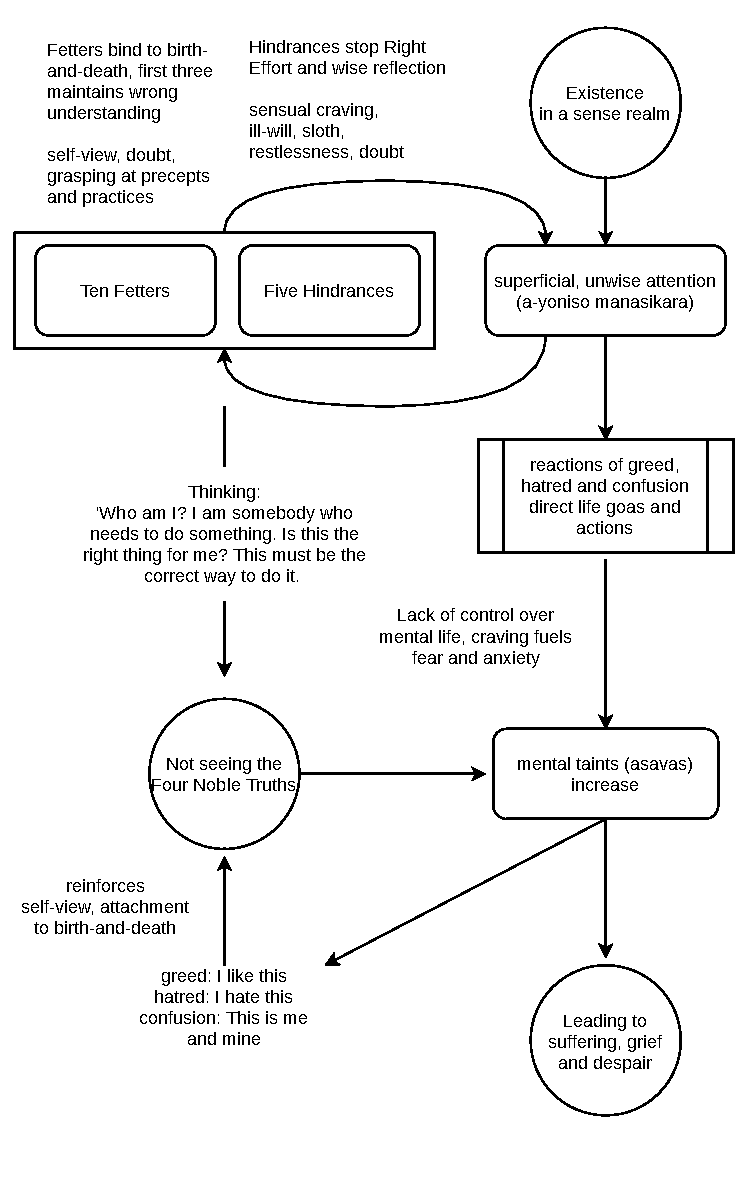
\includegraphics[width=80mm]{leading-to-suffering.pdf}

\end{figure}

\clearpage

\begin{figure}[h]
\caption{Leading to Cessation}\label{fig-leading-to-cessation}

\centering

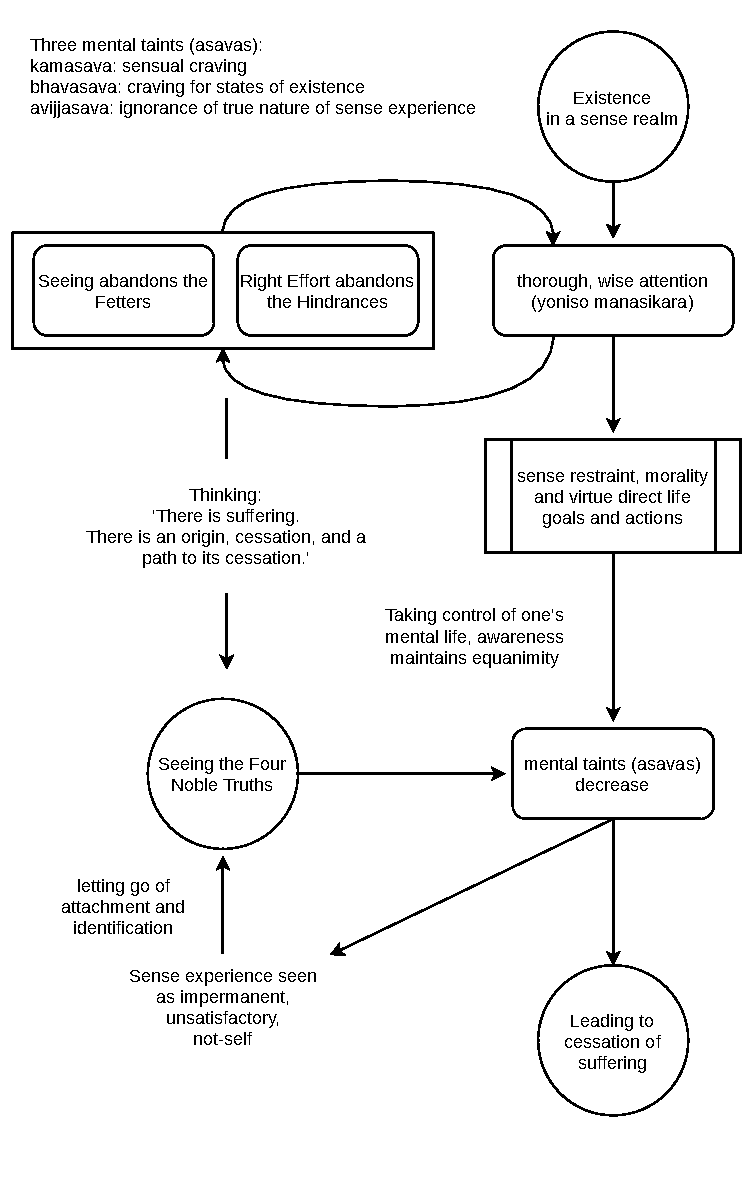
\includegraphics[width=80mm]{leading-to-cessation.pdf}

\end{figure}

% FIXME TODO translate figure

\clearpage

\section{Helyes Nézet}

\keywords{visszatérni a kezdethez, gondolatok megfigyelése}

\noindent Térjünk vissza a légzéshez és folytassuk a meditáció
gyakorlását. Kezdd a gyakorlat elejét az alapokkal, egyszerű lépésekkel
amik vissza terelik a figyelmet a jól ismert keretbe: be- és kilégzés, a
test és annak érzései. Figyeld amit tapasztalsz egy folyamatként, ami
állandó változáson keresztül az egyik érzésből a másikba alakul át.

Minden meditáció egy új kezdet, nem menthetjük el az előző alkalom
eredményeit, hogy most betöltsük a tudást. Ha úgy kezdjük, hogy azt
gondoljuk mi ezt már tudjuk, mondjuk, ha már évek óta gyakoroljuk ezt,
ez egy zárt hozzáálláshoz vezet, ami blokkolja a korábbi megértésünket
is. A múltból származó tapasztalatunk csak úgy értékes, ha a jelenre
vonatkozóan alkalmazzuk. A változó jelen a megértést megújítja és
frissen tartja.

`Ennek a gondolatnak, ennek az érzésnek volt kezdete, most változik, meg
fog szűnni és vége lesz. Meg tudom várni és észre venni azt az
elmúlást?' A közvetlen tapasztalatot így szemlélve, az elme feladja a
vágyat és félelmet az adott állapotokkal kapcsolatban, és megérti őket
mint természetes folyamatok részeit. Nem azt bizonygatjuk magunkban mit
gondolunk az elméről, hanem mintha egy lépést hátralépve szemlélnénk,
éberen tapasztaljuk azt, ahogy van.

Ez a szemlélődés vissza állítja a Helyes Nézetet, mintha egy fordítva, a
fején álló virág vázát valaki újra egyenesen felállítana. Mikor ránézünk
értjük, hogy a vázának melyik része az alja és melyik a teteje.
Szomjasan kívánjuk és ragaszkodunk olyan tapasztalatokhoz, amik mindig
változni fognak, nem hangzik ez feszültségnek és szenvedésnek?
Szerencsére a hiba elkerülhető.

\keywords{korlátok körüli szabadság, lényeg, hála érzet, elárasztva a jó tanáccsal}

A Helyes Nézet megtalálja a teret és szabadságot az élet korlátai és
nyomásai körül. Eleinte talán nem látunk túl sok szabad teret, de a
lényeges dolgokat megvizsgálva észrevehetjük, hogy nincs szükségünk
mindenre amire gondolni tudunk. Megkérdezhetjük, `Megvan, amire
szükségem van erre az egy napra?'

Sorra vehetjük mit használunk a közvetlen környezetünkben -- ruha, étel,
szállás, gyógyszerek. Egyszer mi kapjuk valakitől, vagy engedik, hogy
használjuk, máskor mi adjuk másoknak. `Tudom mennyi elég a mai napra?'
Úgy érzem visszatér a nyugalom, mikor újra felidézem őket, még ha már
jól ismerem ezeket a tényeket.

Felidézve az egyszerű dolgokat, hogy megvan amire szükségünk van, hogy
jól éljük ezt a napot, a hozzáállásunk abban fejezi ki magát, hogy
megnyugvást és hálát érzünk az életért. Nem kell kérned ezt, és nem
tudod akarattal létrehozni. Teret kell adjunk neki a szemléletünkben, és
magától megjelenik.

Hova ez a nagy sietség? Egy egyszerű gyakorlat, hogy megállunk két
percre, nem keresni szórakoztatást és figyelemelterelést, egyszerűen
semmit nem tenni két percig. Figyelheted a lélegzetet, de ez is
választás kérdése. Nem elutasítani az unalmat, mint elme állapotot,
növeli az összpontosításunkat és energiánkat.

A probléma nem az, hogy nincs nem tudunk eleget. A könyvespolcok
túlcsordulnak a jó tanáccsal arról, `hogyan legyünk boldogak'. Ha csak
ez kell, akkor hol a hiba? Ha csak a jó tanácson múlna, már mindannyian
rég megvilágosodtunk volna. Halljuk és olvasunk arról, hogy mi minden jó
dolgot kellene tennünk, milyenféle embernek kellene lennünk: az egyik
könyv szerint legyünk kemények és félelem nélküliek, miközben a másik
szerint univerzális együttérzésre van szükségünk. A szenvedés egy külön
fajtája végigolvasni az egészet.

Vagy talán a \emph{Nibbánára} van szükségünk? Ez a helyes elképzelés? A
szó jelentése \emph{elhűlt, hűvös}, gondolhatunk egy tűzre, ami kialszik
és elhűl. A szomjas vágy, hogy `megszerezzük', csak több tüzelőanyagot
jelent a létesülés hőségéhez és tovább égéséhez.

De a \emph{Nibbána} a létesülésben égés kialvásának hűvössége, tehát
ilyen nem-létesüléssé kellene váljunk? A gondolkodó elme erre az mondja,
`\emph{Mi van?!}' És ez nem is rossz válasz: a Buddha tanítása arra
mutat rá, hogy a gondolkodás és létesülés nem elégséges eszközök ehhez.
Egy újabb állapot vagy gondolat, mikor magunkat látjuk benne, olyan
korlátozó lesz mint a korábbi. Nem abban áll a szabadságunk, hogy a
megfelelő dologgá válunk, hanem a felismerésben, hogy fel tudjuk adni a
kényszert, hogy a folyton valamivé válnunk kelljen.

\clearpage
\figurepagelayout

\begin{figure}[h]
\caption{Experience, Becoming and the Deathless}\label{fig-experience-becoming-deathless}
\bigskip
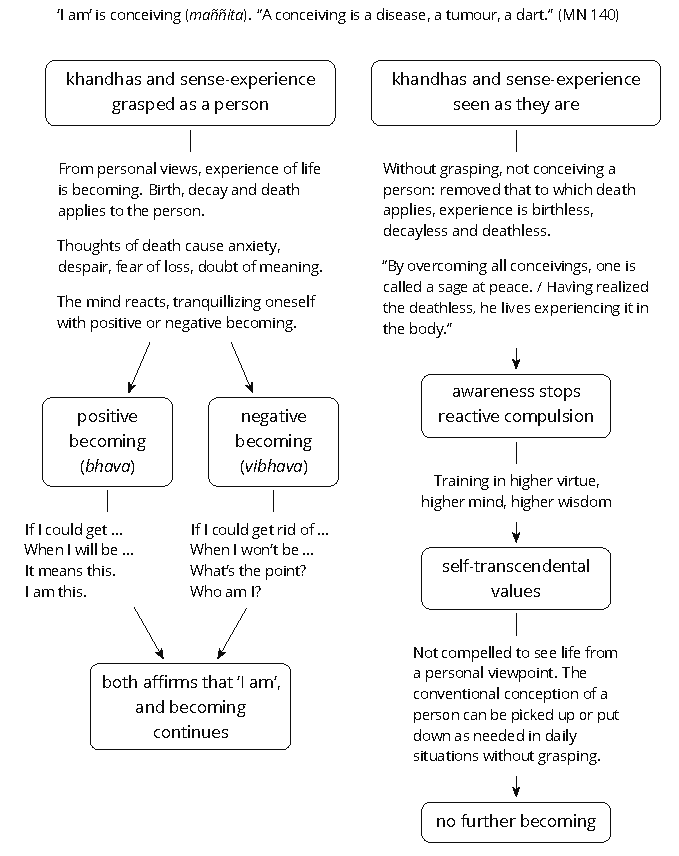
\includegraphics[width=\linewidth]{./manuscript/tex/diagrams/experience-becoming-deathless.pdf}
\end{figure}

{\noindent\footnotesize
Cf.: Chapter 10, Birth, Decay and Death in The Buddha's Teaching: It's Essential\\ Meaning by R. G. de S. Wettimuny
\par}

% TODO: link to Wettimuny book
% TODO: translate figure

\clearpage
\normalpagelayout

\section{Új Szemmel}

\keywords{a tapasztalat felé fordulni, intellektuális tudás, az érzékek figyelése}

\noindent Egy kényszeres hajlamot helyes nézetté változtathatunk át, ha
megkérdezzük, `Hogyan tudom megérteni ezt a tapasztalatot?' Ez a kérdés
a nemes hozzáállás felé irányít minket, amit az Első Nemes Igazság
tartalmaz: `A szenvedést meg kell érteni.' Tedd félre a véleményeket,
melyek válaszként mutatkoznak, és folyton térj vissza ehhez a nyitott
hozzáálláshoz, ami ismeri a jelen pillanatot.

Az öröm és a bánat mind természetes folyamatok, de ha nem értjük őket,
az egyiket jutalomnak tekintjük, a másikat pedig büntetésnek. Úgy tűnik,
az élet sosem igazságos, és mindig úgy tűnik, hogy az irányításunkon
kívül esik.

Ahhoz, hogy megnyissuk a hozzáállásunkat a vizsgálódáshoz, legalább el
kell tudjuk képzelni a lehetőséget, hogy van itt valami amit meg tudunk
tanulni. Egy fordulóponthoz érkezünk, el tudjuk engedni, hogy biztosak
legyünk a véleményeinkben, és megállunk megvizsgálni magát a
tapasztalatot.

Vedd figyelembe, milyen szűk a szemléletünk, amikor azzal a gondolattal
kezdünk, hogy `Ezt már láttam, én ezt ismerem.' Lehet, hogy ez igaz, de
azt veszem észre, hogy amikor ezt az intellektuális információt próbálom
használni egy probléma megoldásához, a figyelmem csupán emlékek,
gondolatok és vélemények körül forog. Amíg magával ragad a múlt, a jelen
tapasztalat elkerüli a figyelmem.

A Buddha utasítása, hogy óvatosan alapozzuk meg a szándékunkat a
meditációra, és tegyük félre a világ ügyeit.

\begin{quote}
Úgy időzik, hogy a testet, {[}az érzéseket, a tudatot, a dhammákban{]} a
keletkezés\ldots{} az elmúlás\ldots{} vagy a keletkezés és az elmúlás
természetét szemléli. Megalapozódik benne az éberség: „van test,
{[}vannak érzések, van tudat, vannak dhammák{]}``, oly mértékben, amely
a puszta tudáshoz és a folytonos éberséghez szükséges. Szabadon időzik,
semmihez sem kötődve a világon.

\bigskip

\quoteRef{%

\href{https://a-buddha-ujja.hu/mn-10/hu/toth-zsuzsanna}{MN 10}, Az
éberség megalapozásáról szóló tanítóbeszéd

}
\end{quote}

A gondolatok és vélemények nem válnak a `saját tudásunkká', de
megérthetjük a megjelenésük és megszűnésük folyamatát. `\emph{Mi} az,
amit éppen teszek? \emph{Hogyan} teszem azt?' Elengedni a merev
álláspontjainkat mutatja az előre vezető utat; úgy fedezzük fel, hogy új
szemmel látunk.\footnote{``Az igazi felfedezőút nem abban áll, hogy új
  tájakat keresünk, hanem abban, hogy új szemmel látunk.'' (Marcel
  Proust)} Az élet talán továbbra sem igazságos és nincs egészen az
irányításunk alatt, de most már ismerünk egy gyakorlást, ami a
különbséget jelenti aközött, hogy ismerjük az elme állapotokat, vagy
teljesen kiborulunk.

Az alapelv az, hogy figyelni az elmét fejleszti az elmét. Az éber
tudatosság megbontja a felgyülemlett hajlamokat. Nem tudhatjuk mi fog
történni holnap, de változás lesz. A `Buddha' szó azt jelenti, `aki
megismer, aki éber'. A tevékenységekben található megelégedettség
forrása az, hogy megbízunk az éber tudatban és gyakoroljuk, hogy ebben
éljünk.

\chapter{Csend}

\section{Jelzés}

\keywords{kapcsolat a környezetünkkel}

\noindent Ketten sétálunk a kolostor bejáratához vezető úton.
Beszélgetünk erről és arról, de amikor belépünk, észrevesszük a csendet
és a párbeszédünk abbamarad. A Dhamma terem a következő ajtón túl van,
és nem akarunk zavarni senkit, aki esetleg odabent meditál. Halkan
bezárjuk magunk mögött az ajtót. Mi az épület egy másik részébe tartunk,
de a Dhamma terem jelentősége nagyobb ennél a hétköznapi feladatnál.

A hallgatás csendje egy implicit kapcsolatot teremt a környezetünkkel.
Az előbbi esetben azzal a személlyel, aki lehet, hogy a Dhamma teremben
ül. Még ha látnánk is, hogy nincs ott senki, akkor is lehalkítanánk a
beszédünket vagy csendben maradnánk. Amikor belépünk, a csend jelzésként
szolgál arra, hogy figyeljünk. Teret adunk az önmagunkon túli
értékeknek, melyeket az szív és elme igazságainak szentelt Dhamma terem
jelképez.

Ebben a környezetben a csend jelzés, ami arra irányít, hogy emlékezzünk
arra, amit a világi értékeken túl van. Amikor egy templomba, kolostorba
vagy más megszentelt helyre lépünk be, a zajos világi ügyeken túlra
tekintünk, túl az önmagunkra irányuló megszokott elfoglaltságunkon.

Elég tapasztalatunk van a zajos csacsogásban ahhoz, hogy tudjuk, a mély
megértés nem abban található. Ezért elcsendesülünk, hogy figyelmünket a
hallgatásnak adhassuk, hogy része legyünk a megértésnek, amit szavakkal
nem tudunk kifejezni. Csendben mozgunk, csendben hallgatunk. Óvatosan
eltávolítjuk magunkat az útból, hogy meghallhassuk a hely üzenetét és
engedjük a cselekvést magáért beszélni. A csend jelenlétet ad, ami nem
elkülönít, hanem magába foglalja a teret és az ott élő más lényeket.
David Whyte szavaival,\footnote{\href{https://www.goodreads.com/quotes/10119971-the-winter-of-listening-no-one-but-me-by-the}{The
  Winter of Listening by David Whyte}}

\begin{quote}
Tartozhatsz mindenhez:\\
csak hallgass csendben.
\end{quote}

\section{Értékes}

\keywords{a csend értéke, nyugalom a csendben}

\noindent A csend azt is kifejezi, mennyire értékeljük amit éppen
teszünk. Csendben lenni és fenntartani a figyelmünket kifejezi az
éberséget és tiszteletet a cselevés iránt. Ez egyaránt egy belső és
külső jelzés: Mások látják, hogy bármi is legyen amit csinálunk, csendre
van szükségünk. Mi is látjuk önmagunkat ahogy csendben vagyunk, mikor
szándékosan visszafogjuk hatásunkat magunkra és a környezetünkre. Ezzel
kommunikáljuk, hogy ahol vagyunk és amit teszünk nagyobb jelentőséggel
bír, mint magunkról csacsogni.

A nyugalom, megértés és csend közeli kapcsolatban állnak egymással.
Felhagyunk a beszéddel és óvatosan figyelünk, hogy vizsgálódjunk és
megértsünk egy jelenséget. A verbális csendet követően, az elme
folytatja, `Miért? Miért?' De amikor összeáll a kép az `Aha!'
pillanatában, az elme megáll a belső párbeszédben és csendben vagyunk,
örömmel tölt el minket a megértés. Ebben az elégedett, nyugodt
hangulatban csendben maradunk. Pillanatnyilag semmi másra nincs
szükségünk.

\begin{quote}
Mint egy tiszta vizű,\\
nyugodt és mély tó, olyan\\
a bölcs, aki miután hallott\\
a dharmákról, lecsendesült.

\bigskip

\quoteRef{%

Dhammapada 82, ford. Fórizs László

}
\end{quote}

\section{Fekvő meditáció módszere}

\noindent A testi nyugalom a fekvő meditáció módszerére a legjellemzőbb.
Ebben a testhelyzetben az izmok teljesen ellazulnak. Habár ez megteremti
a könnyedség és kényelem érzetét, oda kell figyelnünk, hogy elkerüljük
az elalvást. Amikor testileg el vagy fáradva, ez a testtartás nem
javasolt formális meditációra. Ehelyett az ülő, sétáló vagy álló
meditáció megfelelőbb, mivel ezek növelik a test éberségének szintjét az
erőfeszítésen keresztül.

\clearpage
\null\thispagestyle{empty}%
\photoFullBleed{lying-down.jpg}%
\illustration{Fekvő Meditáció Testtartás}%
\label{illus-lying-down-meditation}%
\clearpage

Mielőtt lefeküdnél, határozd meg tisztán a szándékot, hogy éber leszel.
Ez megfelelő hozzáállást teremt, és némi mentális távolságot hoz létre a
napközbeni feladatainktól. Tovább fejleszthetjük a tiszteletteljes
hozzáállást azzal, hogy leborulást végzünk egy Buddha szobor irányába,
és halkan recitálunk egy rövid kántálást.

Egy jóga matrac, vagy puha szőnyeg hasznos, hogy elkerüljük a kemény
padló miatt fájó testrészeket. Ha úgy érzed, hogy a légzésed
akadályozott, miközben a fej hátra hajlik, használj egy kis méretű
párnát, vagy összehajtott törülközőt arra, hogy megtartsa a fejet. Az
ágyban feküdni lehet, hogy túl puha lesz, és a testet az alvásra
emlékezteti.

Engedd a karokat a test mellett pihenni; ha a hasra vagy a mellkasra
helyezed őket, az emelkedő és süllyedő mozgás könnyen elvonja a
figyelmed. Húzd fel a térdeket, hogy a talpak egyenletesen feküdjenek a
szőnyegen és az alsó hátat közelebb engedje a padlóhoz. Ez elkerüli az
ízületekben a feszültséget és segít fenntartani az éberséget.

Tartsd meg ezt a tartást, miközben ellazítod az test izmait és a testi
nyugalmat fejleszted. Irányítsd a figyelmet befelé, használd a légzés
érzetét mint meditációs tárgyat. Kísérletezz a légzéssel. Használd arra,
hogy felélénkítsd az elmét és megőrizd a tiszta éberséget. Ha az elme
elsodródik a szürke tompaság felé, ezt álmosság fogja követni. Egy órát,
vagy időzítő jelzést beállítani hasznos lehet, vagy a meditáció végét
jelezni, vagy mint egy időszakos emlékeztető arra, hogy éber maradj.

\clearpage

\section{A hangok hatása}

\keywords{zajnak kitéve lenni, szabad kognitív kapacitás}

\noindent Ez nem jelenti, hogy a hang nem lehet kellemes. A zene
terápiás hatásai nyilvánvalóak, és segít ellazítani a feszült elmét.
Lehet, hogy \emph{nagyon jó a zene} (a mi véleményünk szerint), de
hányszor tudod meghallgatni egymás után? Ugyanaz a dolog újra és újra,
rövid idő alatt kellemesből fájdalmasba fordul át. Voltál már úgy, hogy
órákig zenét hallgattál, de mégis megkönnyebbülve érezted magad, mikor
kikapcsoltad? `Jó zene, de már hiányzott a csend.'

A hangok bejövő jelek, amik stimulálják az idegrendszert. Egyes hangok
jó érzést kelthetnek egy ideig, pozitív hatással, míg más hangok
irritációt és szétszórtságot okoznak.

A zajos környezet rontja a figyelmünk és intelligenciánk minőségét.
Valószínűleg emlékszel arra, milyen nehéz tisztán gondolkodni amikor a
szomszéd telkén építkezési munkák folynak. A személyes tapasztalaton
túl, orvosi tanulmányok is felmérték, hogy `a szellemi munkavégzés és
látási / hallási figyelem jelentősen csökken'\footnote{\href{https://www.ncbi.nlm.nih.gov/pmc/articles/PMC6901841/}{The
  Effect of Noise Exposure on Cognitive Performance and Brain Activity
  Patterns (ncbi.nlm.nih.gov)}} mikor zajnak vagyunk kitéve.

A mobiltelefonoknak még hangot sem kell kiadniuk, hogy `leszívják az
agyat': egy másik tanulmány azt találta, hogy `a saját telefonunk puszta
jelenléte csökkenti az elérhető szellemi kapacitást'.\footnote{\href{https://www.journals.uchicago.edu/doi/10.1086/691462}{Brain
  Drain: The Mere Presence of One's Own Smartphone Reduces Available
  Cognitive Capacity (journals.uchicago.edu)}}

Nem meglepő, hogy a hagyományos belátás meditációt tanító elvonulások
igyekeznek csendes környezetet teremteni, és arra kérik a résztvevőket,
hogy ne hozzák be a telefonjukat a meditációs terembe, vagy hagyják azt
egy elzárt helyen az egész elvonulás idejére. Adj egy kis szünetet az
idegrendszernek és engedd lecsillapodni. Ne járjon úgy mint a varjú
Szantóka haiku versében,\footnote{\href{https://www.goodreads.com/book/show/931086.Grass_and_Tree_Cairn}{Grass
  and Tree Cairn, Taneda Santoka}}

\begin{quote}
Károg a varjú,\\
csapkod a varjú,\\
nincs ahol megüljön.
\end{quote}

\section{Kántálás}

\keywords{tiszán meghatározni a szándékot, jótékony gondolatok}

\noindent A kolostorban kántálást gyakorlunk a mindennapos közös
meditációk előtt vagy után. Először, amikor egyenként megérkezünk a
Dhamma terembe, csendben három leborulást végzünk a Buddha oltár
irányába. A rangidős szerzetes megcsengeti a harangot, ezzel jelzi a
kántálás kezdetét. Csendben várunk, miközben meggyújtja az oltáron a
gyertyákat és füstölő pálcákat, majd újra meghajlunk. A leborulás közben
mindig csend van.

Együtt elkezdjük a kántálást, összehangolva a hangunkat: a halkat nem
lehet hallani, a hangos túl erős, a hamis kiválik az összhang
harmóniájából. (Egy jó irányelv, ha nem hallod a saját hangod, akkor túl
halkan kántálsz. Ha csak a saját hangodat hallod, túl hangos vagy.)

A kántálások szövegei a Buddhát és a tanításokat idézik fel, ez a
gyakorlat az elmét jótékony gondolatok irányába vezérli. Az ilyen
rendezett, szimbolikus ceremónia a beszéd és test ritmusát használja,
mint alkalmas eszközt arra, hogy kitisztítsa az elmét a meditáció
csendje előtt.

A pontos rutin kolostoronként változik. A Szumédháráma kolostorban
Portugáliában a reggeli mediáció 5 órakor kezdődik. Egy óra ülő
meditációval kezdünk, ami alatt nincs beszéd vagy kántálás. Amikor
belépsz, csend van -- a belső vizsgálódásra szánt megosztott tér. A
meditáció végén a rangidős szerzetes megcsengeti a harangot, amit 15-20
perc kántálás követ.

\section{Unalom}

\keywords{unalom, az eméről tanulni, belső béke, érzéki visszafogottság}

\noindent `Nem unalmas egy idő után?' Időnként egy-egy iskolai program
egy egész osztály gyereket elhoz a kolostorba, hogy csendben
meditáljanak (talán azt remélve, hogy később csendesebbek lesznek). Ők
valószínűleg szörnyen unják magukat. Kezdettől fogva nem érdekelte őket,
hogy ott legyenek, de a gyerekek okosak, és gyakran megtanulják, hogy
hamarabb szabadulnak, ha elviselik a felnőttek furcsa ötleteit.

Amikor a rendszeres látogatóink jönnek meditálni, kezdettől fogva más a
hozzáállásuk ehhez az elmeállapothoz. Úgy érkeznek, hogy érdekli őket,
hogy magukról és az elméjükről tanuljanak. Amikor közelebbről megnézed
azt, ami `unalmas', hamar érdekessé tud válni. Az unalom megváltozik
amint ránézel. `Nem sok minden történik, csak a lélegzés. Probléma ez
nekem? Én hozom létre azt a problémát? Meg tudom állítani, hogy ilyen
problémákat gyártsak magamnak? Itt ülni és lélegezni tulajdonképpen
kellemes érzés.'

Miközben a légzésre való éberséget gyakoroljuk, megjelenik az öröm, ami
az érzékek visszafogottságából születik. Az elme ellazul, és a
gondolkodást engedhetjük megállni. Csendben vizsgáljuk a
tapasztalatunkat, nincs szükség azt kommentálni.

Az unalom a tényezők egy kombinációja: a vágy az izgalomra és
újdonságra, a jelen aktív elutasítása, és a hozzáállás, hogy már tudjuk
mi fog történni. Nem a helyzet magából eredő tulajdonsága, hanem a
képzetlen, nyugtalan elme szokása.

A Buddha a nyugtalanságot ahhoz hasonlította, mint ahogy egy elefánt
érzi magát, amikor az állatidomár első ízben megfékezi azzal, hogy
kiköti egy erős oszlophoz. Az elefánt alkalmatlan a kiképzésre, amíg
folyton arra vágyik, hogy a vadonban kóboroljon amerre csak akar. Egy jó
idomár fokozatosan megfékezi a nyugtalan elefántot, amíg az meg nem
tanul nyugton maradni.\footnote{\href{https://suttacentral.net/mn125}{MN
  125}, The Level of the Tamed} A szuttában, Dzsajaszéna herceg, aki a
palotában él, ahol a figyelemelterelő szórakoztatás veszi őt körbe, el
sem hiszi, hogy a belső békét lehetséges elérni az érzékek visszafogásán
keresztül, hiszen maga sosem tapasztalt még ilyen békét.

A meditációs terem ajtaja mindig nyitva van, bármikor felállhatsz és
kisétálhatsz. De azért vagy ott, mert érezted, hogy a képzetlen elme
állandóan fájdalmas hibákba és gondokba kevert. Ha ezer lépést teszel
ezer irányba, csak elfáradsz, és mérgelődhetsz, hogy miért nem jutottál
sehova. Helyes dolog felismerni a szükséget, hogy saját nyugtalan elménk
idomárai legyünk. Megtanuljuk mi a helyes irány, és arra felé teszünk
lépéseket.

\begin{quote}
A nehezen megfékezhető,\\
csapongó, vágyűzött elme\\
ellenőrzése jó. A megfékezett\\
elme boldogságot hordoz.

\bigskip

\quoteRef{%

Dhammapada 35, ford. Fórizs László

}
\end{quote}

\section{Oltár}

\keywords{szent helyeket létrhozni, egy Buddha oltár szimbólumai}

\noindent Nem mindig készítettem Buddha oltárat a szobában vagy
kunyhóban ahol éppen szállásom volt a kolostorban. Kezdetben azt
gondoltam, hogy az intézményes elvárásokhoz való igazodásban volt
szerepük. Így többnyire figyelmen kívül hagytam őket, és némileg
nehezteltem a képekre és szobrokra. Úgy éreztem mások azt várják el
tőlem, hogy tiszteljem azokat, és ellentartó hozzáállással nem akartam
azt tenni, amit (úgy gondoltam) elvárnak tőlem.

A reakcióm olyan volt, mint az iskolás gyerekeké: elég okos voltam
ahhoz, hogy elviseljem a szimbólumokat, és elég arrogáns ahhoz, hogy azt
higgyem én már tudom mit jelentenek. Aki okosnak gondolja magát,
felületesen elutasít mindent, és unalmassá válik számára a világ. Ez egy
önbutító kombináció. Azt gondolni, hogy \emph{én már tudom}, bezárja az
elmét, így nem tudsz rájönni, hogy valójában nem tudod. A brit
pszichológus Iain McGilchrist ahhoz hasonlítja ezt, mintha beragadtunk
volna egy tükrökből álló labirintusba:\footnote{\href{https://www.goodreads.com/book/show/6968772-the-master-and-his-emissary}{The
  Master and His Emissary: The Divided Brain and the Making of the
  Western World by Iain McGilchrist}} csak azt látod, amit te mondasz
magadnak, és sosem találod meg a kiutat.

Egy kis repedés jelenhetett meg azokon a tükrökön, mert észrevettem,
hogy tulajdonképpen senki nem gondolt rám ilyen ítélettel és elvárással.
Én magam hoztam létre a történet mindkét oldalát, és olyasmi miatt
emésztettem magam amit csak képzeltem.

Egy Buddha oltárt készíteni egy kis teret hoz létre a helyen ahol élünk,
egy emlékeztető arra, hogy álljunk meg a rohanásban és adjunk teret a
felébredésnek. A meditációs terem ugyanezt az üzenetet adja át nekünk a
csenden keresztül. Egy oltár ajándék nekünk, magunktól. Nem azért van,
hogy mások elvárásainak feleljen, vagy akár a Buddhának. A történelmi
Buddha 2600 évvel ezelőtt elhunyt, és túl van azon, hogy tőlünk bármire
is szüksége legyen. Másoknak van elég dolguk amin aggódhatnak, és nem
gondolnak annyit ránk mint azt képzeljük.

\enlargethispage*{\baselineskip}

Emlékszem arra gondoltam, `Miért nincs helyem a Buddha számára ott, ahol
élek?' Neki is láttam levágni néhány fadeszkát és készítettem egy kis
polcot az oltárnak. A Buddha oltárak gyakran elég egyszerűek: egy vagy
több Buddha szobor, gyertyák, füstölő és virágok. A Buddha jelképezi a
felébredett tudatosságot az emberi formában. A gyertyák a bölcsességnek
felelnek meg, ami láthatóvá teszi a dolgokat, mint a fény a sötétségben.
A füstölő eszünkbe juttathatja, amikor a Buddha a jóságról beszélt: `Se
szantálfa, se tagara, se jázmin illata nem száll a szél ellenében, a
jóság viszont szembeszáll a széllel, a jó áthatja az egész
világot.'\footnote{Dhammapada 54, ford. Fórizs László} A virágok az
erényes tettek, boldogság és állandótlanság szimbólumai. Olyanok, mint a
gyakorlásunk: boldogságot hoznak, ha jól gondoskodunk róluk;
elhervadásuk pedig emlékeztet minket az állandótlanságra.

Felajánlom ezeket a vizsgálódó szavakat azzal a szándékkal, hogy
bátorítsanak a gyakorlásban. A tanító a Buddha, a megvilágosító
magyarázatok forrása hozzá vezet vissza. Hálás vagyok azért, hogy a
tanításait egyik generáció a másik után továbbhordozta a sok évszázadon
át a mai napig. Használjuk fel arra, hogy az elme zajos kavargását
átalakítsuk megértő csenddé.


\backmatter

\addcontentsline{toc}{chapter}{\protect\chapternumberline{\thechapter} \protect\emph{Ábrák és Illusztrációk Jegyzéke}}

\listofillustrations*

\vspace*{2\baselineskip}

\listoffigures*

\cleartorecto
\widepagelayout
\thispagestyle{plain}

{\fontsize{9}{11}\selectfont%
\setlength{\parindent}{0pt}%
\raggedright\label{copyright-details}%
\setlength{\parskip}{7pt}%

{\centering

{\LARGE\ccbyncnd}

Ez a Mű a Creative Commons\\
Nevezd meg! - Ne add el! - Ne változtasd! 4.0 Nemzetközi Licenc\\
feltételeinek megfelelően felhasználható.\footnote{%
\href{https://creativecommons.org/licenses/by-nc-nd/4.0/deed.hu}{https://creativecommons.org/licenses/by-nc-nd/4.0/deed.hu}}

}

A műveket szabadon:

\begin{packeditemize}
\item Megoszthatod — másolhatod és terjesztheted a művet bármilyen módon vagy formában
\end{packeditemize}

A jogosult nem vonhatja vissza ezen engedélyeket míg betartod a licenc feltételeit.

Az alábbi feltételekkel:

\begin{packeditemize}
\item Nevezd meg! — A szerzőt megfelelően fel kell tüntetned, hivatkozást kell létrehoznod a licencre és jelezned ha a művön változtatást hajtottál végre. Ezt bármilyen ésszerű módon megteheted, kivéve oly módon ami azt sugallná hogy a jogosult támogat téged vagy a felhasználásod körülményeit.
\item Ne add el! — Nem használhatod a művet üzleti célokra.
\item Ne változtasd! — If you remix, transform, or build upon the material, you may not distribute the modified material.
\end{packeditemize}

Nincsenek további megkötések — Nem szabhatsz meg más jogi vagy technológiai korlátozásokat melyek megakadályoznának bárkit abban hogy ezen licenc által engedélyezett bármely tevékenységeket folytassák.

Megjegyzések:

Nem kell jelen licenc feltételeit követned a művek azon részeinek tekintetében melyek közkincsek vagy ahol a felhasználást egy alkalmazható kivétel vagy korlátozás teszi számodra lehetővé.

Nincs semmiféle garancia. Jelen licencen kívüli engedélyek is szükségesek lehetnek a mű felhasználásához. Példa erre az az eset amikor a mű felhasználását személyiségi, adatvédelmi vagy a jó hírnévre vonatkozó feltételek korlátozzák.

}

\clearpage
\normalpagelayout


\emptyUntilEven

\end{document}
